\documentclass[twoside]{book}

% Packages required by doxygen
\usepackage{fixltx2e}
\usepackage{calc}
\usepackage{doxygen}
\usepackage[export]{adjustbox} % also loads graphicx
\usepackage{graphicx}
\usepackage[utf8]{inputenc}
\usepackage{makeidx}
\usepackage{multicol}
\usepackage{multirow}
\PassOptionsToPackage{warn}{textcomp}
\usepackage{textcomp}
\usepackage[nointegrals]{wasysym}
\usepackage[table]{xcolor}

% NLS support packages
\usepackage[T2A]{fontenc}
\usepackage[russian]{babel}

% Font selection
\usepackage[T1]{fontenc}
\usepackage[scaled=.90]{helvet}
\usepackage{courier}
\usepackage{amssymb}
\usepackage{sectsty}
\renewcommand{\familydefault}{\sfdefault}
\allsectionsfont{%
  \fontseries{bc}\selectfont%
  \color{darkgray}%
}
\renewcommand{\DoxyLabelFont}{%
  \fontseries{bc}\selectfont%
  \color{darkgray}%
}
\newcommand{\+}{\discretionary{\mbox{\scriptsize$\hookleftarrow$}}{}{}}

% Page & text layout
\usepackage{geometry}
\geometry{%
  a4paper,%
  top=2.5cm,%
  bottom=2.5cm,%
  left=2.5cm,%
  right=2.5cm%
}
\tolerance=750
\hfuzz=15pt
\hbadness=750
\setlength{\emergencystretch}{15pt}
\setlength{\parindent}{0cm}
\setlength{\parskip}{3ex plus 2ex minus 2ex}
\makeatletter
\renewcommand{\paragraph}{%
  \@startsection{paragraph}{4}{0ex}{-1.0ex}{1.0ex}{%
    \normalfont\normalsize\bfseries\SS@parafont%
  }%
}
\renewcommand{\subparagraph}{%
  \@startsection{subparagraph}{5}{0ex}{-1.0ex}{1.0ex}{%
    \normalfont\normalsize\bfseries\SS@subparafont%
  }%
}
\makeatother

% Headers & footers
\usepackage{fancyhdr}
\pagestyle{fancyplain}
\fancyhead[LE]{\fancyplain{}{\bfseries\thepage}}
\fancyhead[CE]{\fancyplain{}{}}
\fancyhead[RE]{\fancyplain{}{\bfseries\leftmark}}
\fancyhead[LO]{\fancyplain{}{\bfseries\rightmark}}
\fancyhead[CO]{\fancyplain{}{}}
\fancyhead[RO]{\fancyplain{}{\bfseries\thepage}}
\fancyfoot[LE]{\fancyplain{}{}}
\fancyfoot[CE]{\fancyplain{}{}}
\fancyfoot[RE]{\fancyplain{}{\bfseries\scriptsize Создано системой Doxygen }}
\fancyfoot[LO]{\fancyplain{}{\bfseries\scriptsize Создано системой Doxygen }}
\fancyfoot[CO]{\fancyplain{}{}}
\fancyfoot[RO]{\fancyplain{}{}}
\renewcommand{\footrulewidth}{0.4pt}
\renewcommand{\chaptermark}[1]{%
  \markboth{#1}{}%
}
\renewcommand{\sectionmark}[1]{%
  \markright{\thesection\ #1}%
}

% Indices & bibliography
\usepackage{natbib}
\usepackage[titles]{tocloft}
\setcounter{tocdepth}{3}
\setcounter{secnumdepth}{5}
\makeindex

% Hyperlinks (required, but should be loaded last)
\usepackage{ifpdf}
\ifpdf
  \usepackage[pdftex,pagebackref=true]{hyperref}
\else
  \usepackage[ps2pdf,pagebackref=true]{hyperref}
\fi
\hypersetup{%
  colorlinks=true,%
  linkcolor=blue,%
  citecolor=blue,%
  unicode%
}

% Custom commands
\newcommand{\clearemptydoublepage}{%
  \newpage{\pagestyle{empty}\cleardoublepage}%
}

\usepackage{caption}
\captionsetup{labelsep=space,justification=centering,font={bf},singlelinecheck=off,skip=4pt,position=top}

%===== C O N T E N T S =====

\begin{document}

% Titlepage & ToC
\hypersetup{pageanchor=false,
             bookmarksnumbered=true,
             pdfencoding=unicode
            }
\pagenumbering{alph}
\begin{titlepage}
\vspace*{7cm}
\begin{center}%
{\Large Yenot }\\
\vspace*{1cm}
{\large Создано системой Doxygen 1.8.14}\\
\end{center}
\end{titlepage}
\clearemptydoublepage
\pagenumbering{roman}
\tableofcontents
\clearemptydoublepage
\pagenumbering{arabic}
\hypersetup{pageanchor=true}

%--- Begin generated contents ---
\chapter{Алфавитный указатель групп}
\section{Группы}
Полный список групп.\begin{DoxyCompactList}
\item \contentsline{section}{Yenot}{\pageref{group__yenot}}{}
\begin{DoxyCompactList}
\item \contentsline{section}{Logger.\+cpp}{\pageref{group__loggercpp}}{}
\item \contentsline{section}{Logger.\+h}{\pageref{group__loggerh}}{}
\item \contentsline{section}{Settings.\+cpp}{\pageref{group__settingscpp}}{}
\item \contentsline{section}{Settings.\+h}{\pageref{group__settingsh}}{}
\item \contentsline{section}{Yenot.\+h}{\pageref{group__yenoth}}{}
\end{DoxyCompactList}
\item \contentsline{section}{Core}{\pageref{group__core}}{}
\begin{DoxyCompactList}
\item \contentsline{section}{Core.\+cpp}{\pageref{group__corecpp}}{}
\item \contentsline{section}{Core.\+h}{\pageref{group__coreh}}{}
\item \contentsline{section}{Yenot.\+cpp}{\pageref{group__yenotcpp}}{}
\end{DoxyCompactList}
\item \contentsline{section}{Сервер}{\pageref{group__server}}{}
\begin{DoxyCompactList}
\item \contentsline{section}{Yenot\+Server.\+cpp}{\pageref{group__serveryenotservercpp}}{}
\item \contentsline{section}{Yenot\+Server.\+h}{\pageref{group__serveryenotserverh}}{}
\end{DoxyCompactList}
\end{DoxyCompactList}

\chapter{Алфавитный указатель пространств имен}
\section{Пространства имен}
Полный список пространств имен.\begin{DoxyCompactList}
\item\contentsline{section}{\mbox{\hyperlink{namespaceyenot}{yenot}} \\*Пространство имён с константами }{\pageref{namespaceyenot}}{}
\end{DoxyCompactList}

\chapter{Список файлов}
\section{Файлы}
Полный список файлов.\begin{DoxyCompactList}
\item\contentsline{section}{\mbox{\hyperlink{_core_8cpp}{Core.\+cpp}} \\*ќписание }{\pageref{_core_8cpp}}{}
\item\contentsline{section}{\mbox{\hyperlink{_core_8h}{Core.\+h}} \\*ќписание }{\pageref{_core_8h}}{}
\item\contentsline{section}{\mbox{\hyperlink{_logger_8cpp}{Logger.\+cpp}} }{\pageref{_logger_8cpp}}{}
\item\contentsline{section}{\mbox{\hyperlink{_logger_8h}{Logger.\+h}} \\*Заголовочный файл модуля логирования }{\pageref{_logger_8h}}{}
\item\contentsline{section}{\mbox{\hyperlink{_yenot_8cpp}{Yenot.\+cpp}} \\*Описание }{\pageref{_yenot_8cpp}}{}
\item\contentsline{section}{\mbox{\hyperlink{_yenot_8h}{Yenot.\+h}} \\*\+:D }{\pageref{_yenot_8h}}{}
\end{DoxyCompactList}

\chapter{Группы}
\hypertarget{group__corecpp}{}\section{Core.\+cpp}
\label{group__corecpp}\index{Core.\+cpp@{Core.\+cpp}}
Граф связей класса Core.\+cpp\+:
\nopagebreak
\begin{figure}[H]
\begin{center}
\leavevmode
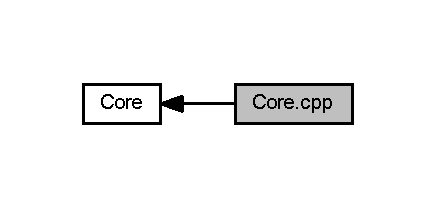
\includegraphics[width=209pt]{group__corecpp}
\end{center}
\end{figure}
\subsection*{Функции}
\begin{DoxyCompactItemize}
\item 
void \mbox{\hyperlink{group__corecpp_gab8ed3baad2f1d9b6b82bf74da9dd3d3a}{noise\+Removal}} (const Mat \&mat\+\_\+in, Mat \&mat\+\_\+out)
\begin{DoxyCompactList}\small\item\em Функция для обработки изображений. \end{DoxyCompactList}\item 
void \mbox{\hyperlink{group__corecpp_ga9e277d82296b5ed9eda6266d8dcc24a3}{line\+Detection}} (const Mat \&mat\+\_\+in, Mat \&mat\+\_\+out)
\begin{DoxyCompactList}\small\item\em Функция для обработки изображений. \end{DoxyCompactList}\item 
void \mbox{\hyperlink{group__corecpp_ga10a0271bceabc9c1a0d736ab93113212}{database\+Add}} (string filename)
\begin{DoxyCompactList}\small\item\em Функция для добавления файла с каскадом в файл с информацией о каскадах \end{DoxyCompactList}\item 
void \mbox{\hyperlink{group__corecpp_ga78cdbfbe907847e78cfb387df76d99f9}{clearning}} (string filename, string variable)
\begin{DoxyCompactList}\small\item\em Функция для очистки дубликатов в векторе \end{DoxyCompactList}\item 
bool \mbox{\hyperlink{group__corecpp_ga76b0b7de3d9fa0de10d66740466ebc14}{detection\+Logo}} (const Mat \&mat\+\_\+logo, string cascadefile)
\begin{DoxyCompactList}\small\item\em Функция для поиска объекта на фото \end{DoxyCompactList}\item 
void \mbox{\hyperlink{group__corecpp_gae99907f19e7f09055012f68347a57d05}{detection}} (const Mat \&mat\+\_\+logo)
\begin{DoxyCompactList}\small\item\em Модуль поиска объектов на фото \end{DoxyCompactList}\item 
void \mbox{\hyperlink{group__corecpp_ga242d25c7a9a1b7212bb890023c8131f5}{settings\+Initialization}} ()
\begin{DoxyCompactList}\small\item\em Модуль настроек. \end{DoxyCompactList}\item 
string \mbox{\hyperlink{group__corecpp_gaa85ae460901348b74381239ce0517d5f}{description}} (string value)
\begin{DoxyCompactList}\small\item\em Функция для поиска описания марки по файлу с каскадом Хаара \end{DoxyCompactList}\item 
void \mbox{\hyperlink{group__corecpp_gafe1c5d9570a4ccddf9b5105997e3ddb4}{canny}} (const Mat \&mat\+\_\+in, Mat \&mat\+\_\+out)
\begin{DoxyCompactList}\small\item\em Функция для обработки изображений. \end{DoxyCompactList}\end{DoxyCompactItemize}


\subsection{Подробное описание}


\subsection{Функции}
\mbox{\Hypertarget{group__corecpp_gafe1c5d9570a4ccddf9b5105997e3ddb4}\label{group__corecpp_gafe1c5d9570a4ccddf9b5105997e3ddb4}} 
\index{Core.\+cpp@{Core.\+cpp}!canny@{canny}}
\index{canny@{canny}!Core.\+cpp@{Core.\+cpp}}
\subsubsection{\texorpdfstring{canny()}{canny()}}
{\footnotesize\ttfamily void canny (\begin{DoxyParamCaption}\item[{const Mat \&}]{mat\+\_\+in,  }\item[{Mat \&}]{mat\+\_\+out }\end{DoxyParamCaption})}



Функция для обработки изображений. 

Поиск границ на изображении. Метод canny.


\begin{DoxyParams}[1]{Аргументы}
\mbox{\tt in}  & {\em mat\+\_\+in} & Матрица с изображением для обработки \\
\hline
\mbox{\tt out}  & {\em mat\+\_\+out} & Матрица с обработанным изображением, которая будет возвращена \\
\hline
\end{DoxyParams}
Создаём матрицы \begin{DoxyVerb}gray - матрица с изображением в оттенках серого

edge - матрица с границами
\end{DoxyVerb}


Преобразуем изображение в оттенки серого

Запускаем алгоритм поиска границ

Возвращаем матрицу с обработанным изображением 

См. определение в файле Core.\+cpp строка 353

\mbox{\Hypertarget{group__corecpp_ga78cdbfbe907847e78cfb387df76d99f9}\label{group__corecpp_ga78cdbfbe907847e78cfb387df76d99f9}} 
\index{Core.\+cpp@{Core.\+cpp}!clearning@{clearning}}
\index{clearning@{clearning}!Core.\+cpp@{Core.\+cpp}}
\subsubsection{\texorpdfstring{clearning()}{clearning()}}
{\footnotesize\ttfamily void clearning (\begin{DoxyParamCaption}\item[{string}]{filename,  }\item[{string}]{variable }\end{DoxyParamCaption})}



Функция для очистки дубликатов в векторе 


\begin{DoxyParams}[1]{Аргументы}
\mbox{\tt in}  & {\em filename} & Название и путь к файлу \\
\hline
\mbox{\tt in}  & {\em variable} & Вектор, в котором нужно удалить дубликаты \\
\hline
\end{DoxyParams}
Создаём вектор

Создаём файловое хранилище

Открываем файловое хранилище для чтения

Записываем данные из файлового хранилища в вектор

Очищаем файловое хранилище

Сортируем значения вектора

Изменяем размер вектора, удаляя дубликаты

Создаём файловое хранилище для записи

Записываем в файловое хранилище обработанный вектор

Очищаем файловое хранилище 

См. определение в файле Core.\+cpp строка 132

\mbox{\Hypertarget{group__corecpp_ga10a0271bceabc9c1a0d736ab93113212}\label{group__corecpp_ga10a0271bceabc9c1a0d736ab93113212}} 
\index{Core.\+cpp@{Core.\+cpp}!database\+Add@{database\+Add}}
\index{database\+Add@{database\+Add}!Core.\+cpp@{Core.\+cpp}}
\subsubsection{\texorpdfstring{database\+Add()}{databaseAdd()}}
{\footnotesize\ttfamily void database\+Add (\begin{DoxyParamCaption}\item[{string}]{filename }\end{DoxyParamCaption})}



Функция для добавления файла с каскадом в файл с информацией о каскадах 


\begin{DoxyParams}[1]{Аргументы}
\mbox{\tt in}  & {\em filename} & Название каскада с расширением \\
\hline
\end{DoxyParams}
Если название файла не задано, то возвращаем ошибку

Создаём вектор

Создаём файловое хранилище

Открываем файловое хранилище для чтения

Записываем данные из файлового хранилища в вектор

Очищаем файловое хранилище

Записываем переменную filename в конец вектора

Создаём файловое хранилище для записи

Записываем в файловое хранилище обработанный вектор

Очищаем файловое хранилище 

См. определение в файле Core.\+cpp строка 90

\mbox{\Hypertarget{group__corecpp_gaa85ae460901348b74381239ce0517d5f}\label{group__corecpp_gaa85ae460901348b74381239ce0517d5f}} 
\index{Core.\+cpp@{Core.\+cpp}!description@{description}}
\index{description@{description}!Core.\+cpp@{Core.\+cpp}}
\subsubsection{\texorpdfstring{description()}{description()}}
{\footnotesize\ttfamily string description (\begin{DoxyParamCaption}\item[{string}]{value }\end{DoxyParamCaption})}



Функция для поиска описания марки по файлу с каскадом Хаара 


\begin{DoxyParams}[1]{Аргументы}
\mbox{\tt in}  & {\em value} & Название файла \\
\hline
\end{DoxyParams}
\begin{DoxyReturn}{Возвращает}
Искомое описание марки 
\end{DoxyReturn}
Создание строковой переменной

Присвоение переменной значения из файла настроек. При отсутствии данных в файле будет присвоено значение D\+E\+S\+C\+R\+I\+P\+T\+I\+O\+N\+\_\+\+N\+O\+T\+\_\+\+F\+O\+U\+ND

Возвращение искомого описания марки 

См. определение в файле Core.\+cpp строка 331

\mbox{\Hypertarget{group__corecpp_gae99907f19e7f09055012f68347a57d05}\label{group__corecpp_gae99907f19e7f09055012f68347a57d05}} 
\index{Core.\+cpp@{Core.\+cpp}!detection@{detection}}
\index{detection@{detection}!Core.\+cpp@{Core.\+cpp}}
\subsubsection{\texorpdfstring{detection()}{detection()}}
{\footnotesize\ttfamily void detection (\begin{DoxyParamCaption}\item[{const Mat \&}]{mat\+\_\+logo }\end{DoxyParamCaption})}



Модуль поиска объектов на фото 

Поиск объектов на фото

Вывод информации


\begin{DoxyParams}[1]{Аргументы}
\mbox{\tt in}  & {\em mat\+\_\+logo} & Матрица с изображением \\
\hline
\end{DoxyParams}
Проверяем. Нужно ли распознавать объект

Создаём вектор ~\newline


Создаём файловое хранилище

Открываем файловое хранилище для чтения

Записываем данные из файлового хранилища в вектор

Очищаем файловое хранилище

Ищем объект на фото

Если объект есть на фото, то пишем в консоль, что объект найден, иначе пишем, что обхект не найден \begin{DoxyVerb}[FOUND] [example.xml] description.

[NOT FOUND] [example.xml]  \end{DoxyVerb}


См. определение в файле Core.\+cpp строка 228

\mbox{\Hypertarget{group__corecpp_ga76b0b7de3d9fa0de10d66740466ebc14}\label{group__corecpp_ga76b0b7de3d9fa0de10d66740466ebc14}} 
\index{Core.\+cpp@{Core.\+cpp}!detection\+Logo@{detection\+Logo}}
\index{detection\+Logo@{detection\+Logo}!Core.\+cpp@{Core.\+cpp}}
\subsubsection{\texorpdfstring{detection\+Logo()}{detectionLogo()}}
{\footnotesize\ttfamily bool detection\+Logo (\begin{DoxyParamCaption}\item[{const Mat \&}]{mat\+\_\+logo,  }\item[{string}]{cascadefile }\end{DoxyParamCaption})}



Функция для поиска объекта на фото 


\begin{DoxyParams}[1]{Аргументы}
\mbox{\tt in}  & {\em mat\+\_\+logo} & Матрица с изображением \\
\hline
\mbox{\tt in}  & {\em cascadefile} & Файл с каскадом \\
\hline
\end{DoxyParams}
\begin{DoxyReturn}{Возвращает}
Результат работы. true -\/ объект найден, false -\/ объект не найден 
\end{DoxyReturn}
Создаём 2 переменные. \begin{DoxyVerb}b_return - возвращаемое значение функции

    true - объект найден на фото

    true - объект не найден на фото

image - матрица с изображением
\end{DoxyVerb}


Создаём переменную для хранения каскада logo\+\_\+cascade

Загружаем каскад (.xml файл)

Если каскад пустой, то возвращаем ошибку

Создаём переменную для распознавания объекта

Загружаем размер шаблона из настроек

Ищем объект на фото

Если объект есть на фото, то возвращаем положительное значение 

См. определение в файле Core.\+cpp строка 173

\mbox{\Hypertarget{group__corecpp_ga9e277d82296b5ed9eda6266d8dcc24a3}\label{group__corecpp_ga9e277d82296b5ed9eda6266d8dcc24a3}} 
\index{Core.\+cpp@{Core.\+cpp}!line\+Detection@{line\+Detection}}
\index{line\+Detection@{line\+Detection}!Core.\+cpp@{Core.\+cpp}}
\subsubsection{\texorpdfstring{line\+Detection()}{lineDetection()}}
{\footnotesize\ttfamily void line\+Detection (\begin{DoxyParamCaption}\item[{const Mat \&}]{mat\+\_\+in,  }\item[{Mat \&}]{mat\+\_\+out }\end{DoxyParamCaption})}



Функция для обработки изображений. 

Проверяет, нужно ли находить линии на изображении.

Для обычного режима используется -\/ canny(mat\+\_\+in, mat\+\_\+out);


\begin{DoxyParams}[1]{Аргументы}
\mbox{\tt in}  & {\em mat\+\_\+in} & Матрица с изображением для обработки \\
\hline
\mbox{\tt out}  & {\em mat\+\_\+out} & Матрица с обработанным изображением, которая будет возвращена \\
\hline
\end{DoxyParams}
Проверяем, нужно ли находить линии на изображении. 

См. определение в файле Core.\+cpp строка 76

\mbox{\Hypertarget{group__corecpp_gab8ed3baad2f1d9b6b82bf74da9dd3d3a}\label{group__corecpp_gab8ed3baad2f1d9b6b82bf74da9dd3d3a}} 
\index{Core.\+cpp@{Core.\+cpp}!noise\+Removal@{noise\+Removal}}
\index{noise\+Removal@{noise\+Removal}!Core.\+cpp@{Core.\+cpp}}
\subsubsection{\texorpdfstring{noise\+Removal()}{noiseRemoval()}}
{\footnotesize\ttfamily void noise\+Removal (\begin{DoxyParamCaption}\item[{const Mat \&}]{mat\+\_\+in,  }\item[{Mat \&}]{mat\+\_\+out }\end{DoxyParamCaption})}



Функция для обработки изображений. 

Проверяет, нужно ли убирать шум на фотографиях.

Также проверяем режим обработки изображений. Быстрый или нет.

Для обычного режима используется двусторонний фильтр -\/ bilateral\+Filter();

Для быстрого режима используется Гауссовый фильтр размытия изображений -\/ Gaussian\+Blur();


\begin{DoxyParams}[1]{Аргументы}
\mbox{\tt in}  & {\em mat\+\_\+in} & Матрица с изображением для обработки \\
\hline
\mbox{\tt out}  & {\em mat\+\_\+out} & Матрица с обработанным изображением, которая будет возвращена \\
\hline
\end{DoxyParams}
Проверяем, нужно ли убирать шум на фотографиях.

Если не нужно убирать шум на фотографиях, то посылаем сообщение в лог

Проверяем режим обработки изображений. Быстрый или нет. \begin{DoxyVerb}Если режим обработки изображений не быстрый, то используем двусторонний фильтр.
\end{DoxyVerb}


иначе \begin{DoxyVerb}Если режим обработки изображений быстрый, то используем Гауссовый фильтр  \end{DoxyVerb}


См. определение в файле Core.\+cpp строка 41

\mbox{\Hypertarget{group__corecpp_ga242d25c7a9a1b7212bb890023c8131f5}\label{group__corecpp_ga242d25c7a9a1b7212bb890023c8131f5}} 
\index{Core.\+cpp@{Core.\+cpp}!settings\+Initialization@{settings\+Initialization}}
\index{settings\+Initialization@{settings\+Initialization}!Core.\+cpp@{Core.\+cpp}}
\subsubsection{\texorpdfstring{settings\+Initialization()}{settingsInitialization()}}
{\footnotesize\ttfamily void settings\+Initialization (\begin{DoxyParamCaption}{ }\end{DoxyParamCaption})}



Модуль настроек. 

При отсутствии файла настроек, создаёт его Если папка N\+A\+M\+E\+\_\+\+D\+A\+T\+A\+B\+A\+SE не найдена и получилось её создать \begin{DoxyVerb}Вывод в лог, что папка создана
\end{DoxyVerb}


иначе \begin{DoxyVerb}Вывод в лог информации, что папку не получилось создать (возможно не достаточно прав или она уже создана)
\end{DoxyVerb}


Проверка наличия файла настроек F\+I\+L\+E\+\_\+\+N\+A\+M\+E\+\_\+\+C\+O\+N\+F\+IG

Если файла нет, то создать его \begin{DoxyVerb}Добавить в файл параметры
\end{DoxyVerb}


Проверка наличия файла с информацией о каскадах F\+I\+L\+E\+\_\+\+N\+A\+M\+E\+\_\+\+D\+A\+T\+A\+B\+A\+SE

Если файла нет, то создать его

Если нет файла C\+A\+R\+\_\+\+M\+O\+D\+E\+L\+\_\+\+E\+X\+A\+M\+P\+L\+E\+\_\+\+F\+I\+LE, то добавить в файл с информацией о каскадах, строку с файлом. Используется для примера 

См. определение в файле Core.\+cpp строка 273


\hypertarget{group__coreh}{}\section{Core.\+h}
\label{group__coreh}\index{Core.\+h@{Core.\+h}}
Граф связей класса Core.\+h\+:
\nopagebreak
\begin{figure}[H]
\begin{center}
\leavevmode
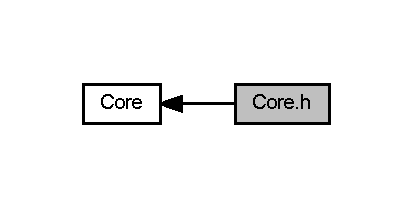
\includegraphics[width=198pt]{group__coreh}
\end{center}
\end{figure}
\subsection*{Функции}
\begin{DoxyCompactItemize}
\item 
void \mbox{\hyperlink{group__coreh_ga438c92819ed0ad4fc2e187ed5f5a2e27}{noise\+Removal}} (const cv\+::\+Mat \&mat\+\_\+in, cv\+::\+Mat \&mat\+\_\+out)
\item 
void \mbox{\hyperlink{group__coreh_gaa7c37c22318217cd913a50800eb336a3}{line\+Detection}} (const cv\+::\+Mat \&mat\+\_\+in, cv\+::\+Mat \&mat\+\_\+out)
\item 
void \mbox{\hyperlink{group__coreh_ga5a4a30ca6128e13ce1ec6efaa23dd6c7}{database\+Add}} (std\+::string filename)
\item 
void \mbox{\hyperlink{group__coreh_gaebd676a1476aa4d75b280db8ae09d11c}{clearning}} (std\+::string filename, std\+::string variable)
\item 
bool \mbox{\hyperlink{group__coreh_gad1ae53e92ff9edcee7a9f35d2956ae57}{detection\+Logo}} (const cv\+::\+Mat \&mat\+\_\+logo, std\+::string cascadefile)
\item 
void \mbox{\hyperlink{group__coreh_ga0ef39a5ada0921b3abf8906957746b86}{detection}} (const cv\+::\+Mat \&mat\+\_\+logo)
\item 
void \mbox{\hyperlink{group__coreh_gaff2d42310702a0aab15af5ad62a59f2b}{canny}} (const cv\+::\+Mat \&mat\+\_\+in, cv\+::\+Mat \&mat\+\_\+out)
\item 
void \mbox{\hyperlink{group__coreh_ga242d25c7a9a1b7212bb890023c8131f5}{settings\+Initialization}} ()
\item 
std\+::string \mbox{\hyperlink{group__coreh_gaad0390ab7aa8f0cac1eee4492e919baf}{description}} (std\+::string value)
\end{DoxyCompactItemize}


\subsection{Подробное описание}


\subsection{Функции}
\mbox{\Hypertarget{group__coreh_gaff2d42310702a0aab15af5ad62a59f2b}\label{group__coreh_gaff2d42310702a0aab15af5ad62a59f2b}} 
\index{Core.\+h@{Core.\+h}!canny@{canny}}
\index{canny@{canny}!Core.\+h@{Core.\+h}}
\subsubsection{\texorpdfstring{canny()}{canny()}}
{\footnotesize\ttfamily void canny (\begin{DoxyParamCaption}\item[{const cv\+::\+Mat \&}]{mat\+\_\+in,  }\item[{cv\+::\+Mat \&}]{mat\+\_\+out }\end{DoxyParamCaption})}

\mbox{\Hypertarget{group__coreh_gaebd676a1476aa4d75b280db8ae09d11c}\label{group__coreh_gaebd676a1476aa4d75b280db8ae09d11c}} 
\index{Core.\+h@{Core.\+h}!clearning@{clearning}}
\index{clearning@{clearning}!Core.\+h@{Core.\+h}}
\subsubsection{\texorpdfstring{clearning()}{clearning()}}
{\footnotesize\ttfamily void clearning (\begin{DoxyParamCaption}\item[{std\+::string}]{filename,  }\item[{std\+::string}]{variable }\end{DoxyParamCaption})}

\mbox{\Hypertarget{group__coreh_ga5a4a30ca6128e13ce1ec6efaa23dd6c7}\label{group__coreh_ga5a4a30ca6128e13ce1ec6efaa23dd6c7}} 
\index{Core.\+h@{Core.\+h}!database\+Add@{database\+Add}}
\index{database\+Add@{database\+Add}!Core.\+h@{Core.\+h}}
\subsubsection{\texorpdfstring{database\+Add()}{databaseAdd()}}
{\footnotesize\ttfamily void database\+Add (\begin{DoxyParamCaption}\item[{std\+::string}]{filename }\end{DoxyParamCaption})}

\mbox{\Hypertarget{group__coreh_gaad0390ab7aa8f0cac1eee4492e919baf}\label{group__coreh_gaad0390ab7aa8f0cac1eee4492e919baf}} 
\index{Core.\+h@{Core.\+h}!description@{description}}
\index{description@{description}!Core.\+h@{Core.\+h}}
\subsubsection{\texorpdfstring{description()}{description()}}
{\footnotesize\ttfamily std\+::string description (\begin{DoxyParamCaption}\item[{std\+::string}]{value }\end{DoxyParamCaption})}

\mbox{\Hypertarget{group__coreh_ga0ef39a5ada0921b3abf8906957746b86}\label{group__coreh_ga0ef39a5ada0921b3abf8906957746b86}} 
\index{Core.\+h@{Core.\+h}!detection@{detection}}
\index{detection@{detection}!Core.\+h@{Core.\+h}}
\subsubsection{\texorpdfstring{detection()}{detection()}}
{\footnotesize\ttfamily void detection (\begin{DoxyParamCaption}\item[{const cv\+::\+Mat \&}]{mat\+\_\+logo }\end{DoxyParamCaption})}

\mbox{\Hypertarget{group__coreh_gad1ae53e92ff9edcee7a9f35d2956ae57}\label{group__coreh_gad1ae53e92ff9edcee7a9f35d2956ae57}} 
\index{Core.\+h@{Core.\+h}!detection\+Logo@{detection\+Logo}}
\index{detection\+Logo@{detection\+Logo}!Core.\+h@{Core.\+h}}
\subsubsection{\texorpdfstring{detection\+Logo()}{detectionLogo()}}
{\footnotesize\ttfamily bool detection\+Logo (\begin{DoxyParamCaption}\item[{const cv\+::\+Mat \&}]{mat\+\_\+logo,  }\item[{std\+::string}]{cascadefile }\end{DoxyParamCaption})}

\mbox{\Hypertarget{group__coreh_gaa7c37c22318217cd913a50800eb336a3}\label{group__coreh_gaa7c37c22318217cd913a50800eb336a3}} 
\index{Core.\+h@{Core.\+h}!line\+Detection@{line\+Detection}}
\index{line\+Detection@{line\+Detection}!Core.\+h@{Core.\+h}}
\subsubsection{\texorpdfstring{line\+Detection()}{lineDetection()}}
{\footnotesize\ttfamily void line\+Detection (\begin{DoxyParamCaption}\item[{const cv\+::\+Mat \&}]{mat\+\_\+in,  }\item[{cv\+::\+Mat \&}]{mat\+\_\+out }\end{DoxyParamCaption})}

\mbox{\Hypertarget{group__coreh_ga438c92819ed0ad4fc2e187ed5f5a2e27}\label{group__coreh_ga438c92819ed0ad4fc2e187ed5f5a2e27}} 
\index{Core.\+h@{Core.\+h}!noise\+Removal@{noise\+Removal}}
\index{noise\+Removal@{noise\+Removal}!Core.\+h@{Core.\+h}}
\subsubsection{\texorpdfstring{noise\+Removal()}{noiseRemoval()}}
{\footnotesize\ttfamily void noise\+Removal (\begin{DoxyParamCaption}\item[{const cv\+::\+Mat \&}]{mat\+\_\+in,  }\item[{cv\+::\+Mat \&}]{mat\+\_\+out }\end{DoxyParamCaption})}

\mbox{\Hypertarget{group__coreh_ga242d25c7a9a1b7212bb890023c8131f5}\label{group__coreh_ga242d25c7a9a1b7212bb890023c8131f5}} 
\index{Core.\+h@{Core.\+h}!settings\+Initialization@{settings\+Initialization}}
\index{settings\+Initialization@{settings\+Initialization}!Core.\+h@{Core.\+h}}
\subsubsection{\texorpdfstring{settings\+Initialization()}{settingsInitialization()}}
{\footnotesize\ttfamily void settings\+Initialization (\begin{DoxyParamCaption}{ }\end{DoxyParamCaption})}



См. определение в файле Core.\+cpp строка 158


\hypertarget{group__loggercpp}{}\section{Logger.\+cpp}
\label{group__loggercpp}\index{Logger.\+cpp@{Logger.\+cpp}}
Граф связей класса Logger.\+cpp\+:
\nopagebreak
\begin{figure}[H]
\begin{center}
\leavevmode
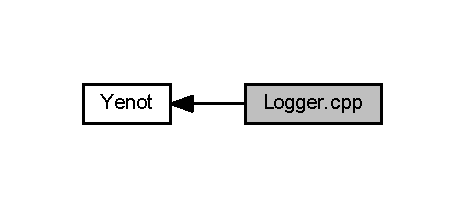
\includegraphics[width=223pt]{group__loggercpp}
\end{center}
\end{figure}
\subsection*{Функции}
\begin{DoxyCompactItemize}
\item 
void \mbox{\hyperlink{group__loggercpp_ga0d6abeb129096910c85ae6cba8bb59cf}{logger}} (char $\ast$level, char $\ast$text)
\begin{DoxyCompactList}\small\item\em Основная функция для логирования \end{DoxyCompactList}\end{DoxyCompactItemize}


\subsection{Подробное описание}


\subsection{Функции}
\mbox{\Hypertarget{group__loggercpp_ga0d6abeb129096910c85ae6cba8bb59cf}\label{group__loggercpp_ga0d6abeb129096910c85ae6cba8bb59cf}} 
\index{Logger.\+cpp@{Logger.\+cpp}!logger@{logger}}
\index{logger@{logger}!Logger.\+cpp@{Logger.\+cpp}}
\subsubsection{\texorpdfstring{logger()}{logger()}}
{\footnotesize\ttfamily void logger (\begin{DoxyParamCaption}\item[{char $\ast$}]{level,  }\item[{char $\ast$}]{text }\end{DoxyParamCaption})}



Основная функция для логирования 

Логирование возможно с разными уровнями и с выводом времени


\begin{DoxyParams}[1]{Аргументы}
\mbox{\tt in}  & {\em level} & Уровень логирования \\
\hline
\mbox{\tt in}  & {\em text} & Текст для логирования \\
\hline
\end{DoxyParams}
Проверяем, нужно ли логировать.

Проверка наличия файла с выводом лога в папке.

Если файл не найден, то создаём его ~\newline
~\newline
~\newline
 Проверка, нужно ли логировать с выводом времени

Если нужно ли логировать с выводом времени, то \begin{DoxyVerb}Создаём строки, которые будут хранить в себе значения текущего времени

Создаём структуру SYSTEMTIME из которой будем брать текущее время

Получаем текущее время системы и по адресу присваиваем значение структуре time

Помещаем текущее время системы в строки.

Открываем файл для логирования. Открываем файл для записи в конце.

Записываем данные в файл

Закрываем файл
\end{DoxyVerb}


иначе \begin{DoxyVerb}Открываем файл для логирования. Открываем файл для записи в конце.

Записываем данные в файл

Закрываем файл  \end{DoxyVerb}


Записываем данные в файл.

Пример\+: 
\begin{DoxyCode}
[2018/05/02 17:17:03] [WARN]Folder created.
\end{DoxyCode}
 ~\newline
 Записываем данные в файл.

Пример\+: 
\begin{DoxyCode}
[WARN]Folder created.
\end{DoxyCode}
 

См. определение в файле Logger.\+cpp строка 29


\hypertarget{group__loggerh}{}\section{Logger.\+h}
\label{group__loggerh}\index{Logger.\+h@{Logger.\+h}}
Граф связей класса Logger.\+h\+:
\nopagebreak
\begin{figure}[H]
\begin{center}
\leavevmode
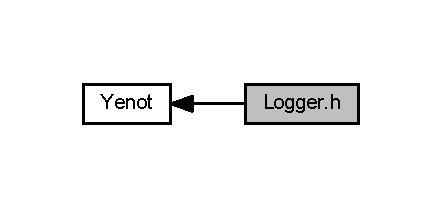
\includegraphics[width=212pt]{group__loggerh}
\end{center}
\end{figure}
\subsection*{Функции}
\begin{DoxyCompactItemize}
\item 
void \mbox{\hyperlink{group__loggerh_ga0d6abeb129096910c85ae6cba8bb59cf}{logger}} (char $\ast$level, char $\ast$text)
\begin{DoxyCompactList}\small\item\em Основная функция для логирования \end{DoxyCompactList}\end{DoxyCompactItemize}


\subsection{Подробное описание}


\subsection{Функции}
\mbox{\Hypertarget{group__loggerh_ga0d6abeb129096910c85ae6cba8bb59cf}\label{group__loggerh_ga0d6abeb129096910c85ae6cba8bb59cf}} 
\index{Logger.\+h@{Logger.\+h}!logger@{logger}}
\index{logger@{logger}!Logger.\+h@{Logger.\+h}}
\subsubsection{\texorpdfstring{logger()}{logger()}}
{\footnotesize\ttfamily void logger (\begin{DoxyParamCaption}\item[{char $\ast$}]{level,  }\item[{char $\ast$}]{text }\end{DoxyParamCaption})}



Основная функция для логирования 

Логирование возможно с разными уровнями и с выводом времени


\begin{DoxyParams}[1]{Аргументы}
\mbox{\tt in}  & {\em level} & Уровень логирования \\
\hline
\mbox{\tt in}  & {\em text} & Текст для логирования \\
\hline
\end{DoxyParams}
Проверяем, нужно ли логировать.

Проверка наличия файла с выводом лога в папке.

Если файл не найден, то создаём его ~\newline
~\newline
~\newline
 Проверка, нужно ли логировать с выводом времени

Если нужно ли логировать с выводом времени, то \begin{DoxyVerb}Создаём строки, которые будут хранить в себе значения текущего времени

Создаём структуру SYSTEMTIME из которой будем брать текущее время

Получаем текущее время системы и по адресу присваиваем значение структуре time

Помещаем текущее время системы в строки.

Открываем файл для логирования. Открываем файл для записи в конце.

Записываем данные в файл

Закрываем файл
\end{DoxyVerb}


иначе \begin{DoxyVerb}Открываем файл для логирования. Открываем файл для записи в конце.

Записываем данные в файл

Закрываем файл  \end{DoxyVerb}


Записываем данные в файл.

Пример\+: 
\begin{DoxyCode}
[2018/05/02 17:17:03] [WARN]Folder created.
\end{DoxyCode}
 ~\newline
 Записываем данные в файл.

Пример\+: 
\begin{DoxyCode}
[WARN]Folder created.
\end{DoxyCode}
 

См. определение в файле Logger.\+cpp строка 29


\hypertarget{group__settingscpp}{}\section{Settings.\+cpp}
\label{group__settingscpp}\index{Settings.\+cpp@{Settings.\+cpp}}
Граф связей класса Settings.\+cpp\+:
\nopagebreak
\begin{figure}[H]
\begin{center}
\leavevmode
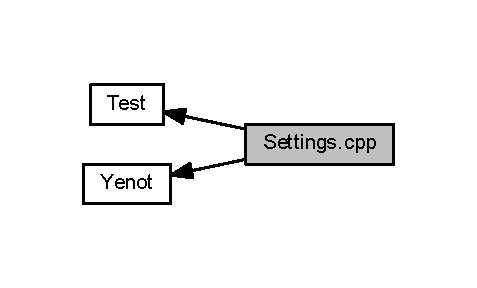
\includegraphics[width=229pt]{group__settingscpp}
\end{center}
\end{figure}
\subsection*{Функции}
\begin{DoxyCompactItemize}
\item 
string \mbox{\hyperlink{group__settingscpp_ga50535cebf45c8d7cbffd29274699e5f5}{get\+Settings\+String}} (char $\ast$block, char $\ast$value, char $\ast$ch\+\_\+return\+\_\+default)
\begin{DoxyCompactList}\small\item\em Получить строку из файла настроек \end{DoxyCompactList}\item 
int \mbox{\hyperlink{group__settingscpp_ga0a2fe94de4037eda33c49fe332970891}{get\+Settings}} (char $\ast$block, char $\ast$value, int i\+\_\+return\+\_\+default)
\begin{DoxyCompactList}\small\item\em Получить число из файла настроек \end{DoxyCompactList}\item 
void \mbox{\hyperlink{group__settingscpp_ga463e32ccb37f9478b0e62ee0d21c5999}{set\+Settings}} (char $\ast$block, char $\ast$value, char $\ast$text)
\begin{DoxyCompactList}\small\item\em Сохранить переменную в файл настроек \end{DoxyCompactList}\item 
bool \mbox{\hyperlink{group__settingscpp_ga2dd1bc039652a0480c444957d416b6a6}{check\+File}} (char $\ast$filename)
\begin{DoxyCompactList}\small\item\em Проверка файла \end{DoxyCompactList}\item 
bool \mbox{\hyperlink{group__settingscpp_ga64f8c9899c815dc180b2b564c0d05762}{check\+File}} (string filename)
\begin{DoxyCompactList}\small\item\em Проверка файла \end{DoxyCompactList}\item 
void \mbox{\hyperlink{group__settingscpp_ga5ac0cd45ecb6e65e3ace40687d6ee8bc}{create\+Dir}} (string namedir)
\begin{DoxyCompactList}\small\item\em Функция для создания директории \end{DoxyCompactList}\item 
void \mbox{\hyperlink{group__settingscpp_ga8f34a2030acfb5567678ab2bba25f3c1}{create\+File}} (char $\ast$file\+\_\+name)
\begin{DoxyCompactList}\small\item\em Функция для создания файла \end{DoxyCompactList}\end{DoxyCompactItemize}


\subsection{Подробное описание}


\subsection{Функции}
\mbox{\Hypertarget{group__settingscpp_ga2dd1bc039652a0480c444957d416b6a6}\label{group__settingscpp_ga2dd1bc039652a0480c444957d416b6a6}} 
\index{Settings.\+cpp@{Settings.\+cpp}!check\+File@{check\+File}}
\index{check\+File@{check\+File}!Settings.\+cpp@{Settings.\+cpp}}
\subsubsection{\texorpdfstring{check\+File()}{checkFile()}\hspace{0.1cm}{\footnotesize\ttfamily [1/2]}}
{\footnotesize\ttfamily bool check\+File (\begin{DoxyParamCaption}\item[{char $\ast$}]{filename }\end{DoxyParamCaption})}



Проверка файла 


\begin{DoxyParams}[1]{Аргументы}
\mbox{\tt in}  & {\em filename} & Название файла \\
\hline
\end{DoxyParams}
\begin{DoxyReturn}{Возвращает}
true -\/ файл найден, false -\/ файл не найден. 
\end{DoxyReturn}


См. определение в файле Settings.\+cpp строка 62

\mbox{\Hypertarget{group__settingscpp_ga64f8c9899c815dc180b2b564c0d05762}\label{group__settingscpp_ga64f8c9899c815dc180b2b564c0d05762}} 
\index{Settings.\+cpp@{Settings.\+cpp}!check\+File@{check\+File}}
\index{check\+File@{check\+File}!Settings.\+cpp@{Settings.\+cpp}}
\subsubsection{\texorpdfstring{check\+File()}{checkFile()}\hspace{0.1cm}{\footnotesize\ttfamily [2/2]}}
{\footnotesize\ttfamily bool check\+File (\begin{DoxyParamCaption}\item[{string}]{filename }\end{DoxyParamCaption})}



Проверка файла 


\begin{DoxyParams}[1]{Аргументы}
\mbox{\tt in}  & {\em filename} & Название файла \\
\hline
\end{DoxyParams}
\begin{DoxyReturn}{Возвращает}
true -\/ файл найден, false -\/ файл не найден. 
\end{DoxyReturn}


См. определение в файле Settings.\+cpp строка 76

\mbox{\Hypertarget{group__settingscpp_ga5ac0cd45ecb6e65e3ace40687d6ee8bc}\label{group__settingscpp_ga5ac0cd45ecb6e65e3ace40687d6ee8bc}} 
\index{Settings.\+cpp@{Settings.\+cpp}!create\+Dir@{create\+Dir}}
\index{create\+Dir@{create\+Dir}!Settings.\+cpp@{Settings.\+cpp}}
\subsubsection{\texorpdfstring{create\+Dir()}{createDir()}}
{\footnotesize\ttfamily void create\+Dir (\begin{DoxyParamCaption}\item[{string}]{namedir }\end{DoxyParamCaption})}



Функция для создания директории 


\begin{DoxyParams}[1]{Аргументы}
\mbox{\tt in}  & {\em namedir} & Путь и название директории \\
\hline
\end{DoxyParams}
Если успешно создали директорию, то\+: \begin{DoxyVerb}Вывод в лог, что получилось создать директорию
\end{DoxyVerb}


иначе\+: \begin{DoxyVerb}Вывод в лог, что не получилось создать директорию

Возможно это связано с тем, что нет прав на создание директории или директория уже есть  \end{DoxyVerb}


См. определение в файле Settings.\+cpp строка 90

\mbox{\Hypertarget{group__settingscpp_ga8f34a2030acfb5567678ab2bba25f3c1}\label{group__settingscpp_ga8f34a2030acfb5567678ab2bba25f3c1}} 
\index{Settings.\+cpp@{Settings.\+cpp}!create\+File@{create\+File}}
\index{create\+File@{create\+File}!Settings.\+cpp@{Settings.\+cpp}}
\subsubsection{\texorpdfstring{create\+File()}{createFile()}}
{\footnotesize\ttfamily void create\+File (\begin{DoxyParamCaption}\item[{char $\ast$}]{file\+\_\+name }\end{DoxyParamCaption})}



Функция для создания файла 


\begin{DoxyParams}[1]{Аргументы}
\mbox{\tt in}  & {\em file\+\_\+name} & Путь и название файла \\
\hline
\end{DoxyParams}


См. определение в файле Settings.\+cpp строка 111

\mbox{\Hypertarget{group__settingscpp_ga0a2fe94de4037eda33c49fe332970891}\label{group__settingscpp_ga0a2fe94de4037eda33c49fe332970891}} 
\index{Settings.\+cpp@{Settings.\+cpp}!get\+Settings@{get\+Settings}}
\index{get\+Settings@{get\+Settings}!Settings.\+cpp@{Settings.\+cpp}}
\subsubsection{\texorpdfstring{get\+Settings()}{getSettings()}}
{\footnotesize\ttfamily int get\+Settings (\begin{DoxyParamCaption}\item[{char $\ast$}]{block,  }\item[{char $\ast$}]{value,  }\item[{int}]{i\+\_\+return\+\_\+default }\end{DoxyParamCaption})}



Получить число из файла настроек 


\begin{DoxyParams}[1]{Аргументы}
\mbox{\tt in}  & {\em block} & Блок файла настроек \\
\hline
\mbox{\tt in}  & {\em value} & Искомая переменная \\
\hline
\mbox{\tt in}  & {\em i\+\_\+return\+\_\+default} & Значение, если переменная не найдена в файле настроек \\
\hline
\end{DoxyParams}
\begin{DoxyReturn}{Возвращает}
Число из файла настроек 
\end{DoxyReturn}


См. определение в файле Settings.\+cpp строка 43

\mbox{\Hypertarget{group__settingscpp_ga50535cebf45c8d7cbffd29274699e5f5}\label{group__settingscpp_ga50535cebf45c8d7cbffd29274699e5f5}} 
\index{Settings.\+cpp@{Settings.\+cpp}!get\+Settings\+String@{get\+Settings\+String}}
\index{get\+Settings\+String@{get\+Settings\+String}!Settings.\+cpp@{Settings.\+cpp}}
\subsubsection{\texorpdfstring{get\+Settings\+String()}{getSettingsString()}}
{\footnotesize\ttfamily string get\+Settings\+String (\begin{DoxyParamCaption}\item[{char $\ast$}]{block,  }\item[{char $\ast$}]{value,  }\item[{char $\ast$}]{ch\+\_\+return\+\_\+default }\end{DoxyParamCaption})}



Получить строку из файла настроек 


\begin{DoxyParams}[1]{Аргументы}
\mbox{\tt in}  & {\em block} & Блок файла настроек \\
\hline
\mbox{\tt in}  & {\em value} & Искомая переменная \\
\hline
\mbox{\tt in}  & {\em ch\+\_\+return\+\_\+default} & Значение, если переменная не найдена в файле настроек \\
\hline
\end{DoxyParams}
\begin{DoxyReturn}{Возвращает}
Строка из файла настроек 
\end{DoxyReturn}


См. определение в файле Settings.\+cpp строка 30

\mbox{\Hypertarget{group__settingscpp_ga463e32ccb37f9478b0e62ee0d21c5999}\label{group__settingscpp_ga463e32ccb37f9478b0e62ee0d21c5999}} 
\index{Settings.\+cpp@{Settings.\+cpp}!set\+Settings@{set\+Settings}}
\index{set\+Settings@{set\+Settings}!Settings.\+cpp@{Settings.\+cpp}}
\subsubsection{\texorpdfstring{set\+Settings()}{setSettings()}}
{\footnotesize\ttfamily void set\+Settings (\begin{DoxyParamCaption}\item[{char $\ast$}]{block,  }\item[{char $\ast$}]{value,  }\item[{char $\ast$}]{text }\end{DoxyParamCaption})}



Сохранить переменную в файл настроек 


\begin{DoxyParams}[1]{Аргументы}
\mbox{\tt in}  & {\em block} & Блок файла настроек \\
\hline
\mbox{\tt in}  & {\em value} & Переменная \\
\hline
\mbox{\tt in}  & {\em text} & Значение переменной \\
\hline
\end{DoxyParams}


См. определение в файле Settings.\+cpp строка 53


\hypertarget{group__settingsh}{}\section{Settings.\+h}
\label{group__settingsh}\index{Settings.\+h@{Settings.\+h}}
Граф связей класса Settings.\+h\+:
\nopagebreak
\begin{figure}[H]
\begin{center}
\leavevmode
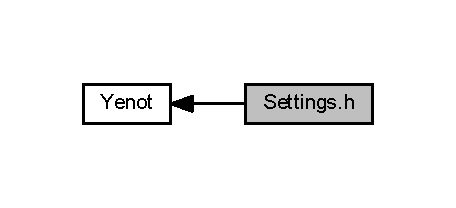
\includegraphics[width=219pt]{group__settingsh}
\end{center}
\end{figure}
\subsection*{Функции}
\begin{DoxyCompactItemize}
\item 
std\+::string \mbox{\hyperlink{group__settingsh_ga3a0f1e87eb01bdd16c4a7e365aa283eb}{get\+Settings\+String}} (char $\ast$block, char $\ast$value, char $\ast$ch\+\_\+return\+\_\+default)
\begin{DoxyCompactList}\small\item\em Получить строку из файла настроек \end{DoxyCompactList}\item 
int \mbox{\hyperlink{group__settingsh_ga0a2fe94de4037eda33c49fe332970891}{get\+Settings}} (char $\ast$block, char $\ast$value, int i\+\_\+return\+\_\+default)
\begin{DoxyCompactList}\small\item\em Получить число из файла настроек \end{DoxyCompactList}\item 
void \mbox{\hyperlink{group__settingsh_ga463e32ccb37f9478b0e62ee0d21c5999}{set\+Settings}} (char $\ast$block, char $\ast$value, char $\ast$text)
\begin{DoxyCompactList}\small\item\em Сохранить переменную в файл настроек \end{DoxyCompactList}\item 
bool \mbox{\hyperlink{group__settingsh_ga2dd1bc039652a0480c444957d416b6a6}{check\+File}} (char $\ast$filename)
\begin{DoxyCompactList}\small\item\em Проверка файла \end{DoxyCompactList}\item 
bool \mbox{\hyperlink{group__settingsh_ga147bed619c6314e960320c1bcb40ed91}{check\+File}} (std\+::string filename)
\begin{DoxyCompactList}\small\item\em Проверка файла \end{DoxyCompactList}\item 
void \mbox{\hyperlink{group__settingsh_ga912b67f6f6b05abadd055a379dd84864}{create\+Dir}} (std\+::string namedir)
\begin{DoxyCompactList}\small\item\em Функция для создания директории \end{DoxyCompactList}\item 
void \mbox{\hyperlink{group__settingsh_ga8f34a2030acfb5567678ab2bba25f3c1}{create\+File}} (char $\ast$file\+\_\+name)
\begin{DoxyCompactList}\small\item\em Функция для создания файла \end{DoxyCompactList}\end{DoxyCompactItemize}


\subsection{Подробное описание}


\subsection{Функции}
\mbox{\Hypertarget{group__settingsh_ga2dd1bc039652a0480c444957d416b6a6}\label{group__settingsh_ga2dd1bc039652a0480c444957d416b6a6}} 
\index{Settings.\+h@{Settings.\+h}!check\+File@{check\+File}}
\index{check\+File@{check\+File}!Settings.\+h@{Settings.\+h}}
\subsubsection{\texorpdfstring{check\+File()}{checkFile()}\hspace{0.1cm}{\footnotesize\ttfamily [1/2]}}
{\footnotesize\ttfamily bool check\+File (\begin{DoxyParamCaption}\item[{char $\ast$}]{filename }\end{DoxyParamCaption})}



Проверка файла 


\begin{DoxyParams}[1]{Аргументы}
\mbox{\tt in}  & {\em filename} & Название файла \\
\hline
\end{DoxyParams}
\begin{DoxyReturn}{Возвращает}
true -\/ файл найден, false -\/ файл не найден. 
\end{DoxyReturn}


См. определение в файле server/src/\+Settings.\+cpp строка 62

\mbox{\Hypertarget{group__settingsh_ga147bed619c6314e960320c1bcb40ed91}\label{group__settingsh_ga147bed619c6314e960320c1bcb40ed91}} 
\index{Settings.\+h@{Settings.\+h}!check\+File@{check\+File}}
\index{check\+File@{check\+File}!Settings.\+h@{Settings.\+h}}
\subsubsection{\texorpdfstring{check\+File()}{checkFile()}\hspace{0.1cm}{\footnotesize\ttfamily [2/2]}}
{\footnotesize\ttfamily bool check\+File (\begin{DoxyParamCaption}\item[{std\+::string}]{filename }\end{DoxyParamCaption})}



Проверка файла 


\begin{DoxyParams}[1]{Аргументы}
\mbox{\tt in}  & {\em filename} & Название файла \\
\hline
\end{DoxyParams}
\begin{DoxyReturn}{Возвращает}
true -\/ файл найден, false -\/ файл не найден. 
\end{DoxyReturn}
\mbox{\Hypertarget{group__settingsh_ga912b67f6f6b05abadd055a379dd84864}\label{group__settingsh_ga912b67f6f6b05abadd055a379dd84864}} 
\index{Settings.\+h@{Settings.\+h}!create\+Dir@{create\+Dir}}
\index{create\+Dir@{create\+Dir}!Settings.\+h@{Settings.\+h}}
\subsubsection{\texorpdfstring{create\+Dir()}{createDir()}}
{\footnotesize\ttfamily void create\+Dir (\begin{DoxyParamCaption}\item[{std\+::string}]{namedir }\end{DoxyParamCaption})}



Функция для создания директории 


\begin{DoxyParams}[1]{Аргументы}
\mbox{\tt in}  & {\em namedir} & Путь и название директории \\
\hline
\end{DoxyParams}
\mbox{\Hypertarget{group__settingsh_ga8f34a2030acfb5567678ab2bba25f3c1}\label{group__settingsh_ga8f34a2030acfb5567678ab2bba25f3c1}} 
\index{Settings.\+h@{Settings.\+h}!create\+File@{create\+File}}
\index{create\+File@{create\+File}!Settings.\+h@{Settings.\+h}}
\subsubsection{\texorpdfstring{create\+File()}{createFile()}}
{\footnotesize\ttfamily void create\+File (\begin{DoxyParamCaption}\item[{char $\ast$}]{file\+\_\+name }\end{DoxyParamCaption})}



Функция для создания файла 


\begin{DoxyParams}[1]{Аргументы}
\mbox{\tt in}  & {\em file\+\_\+name} & Путь и название файла \\
\hline
\end{DoxyParams}


См. определение в файле server/src/\+Settings.\+cpp строка 111

\mbox{\Hypertarget{group__settingsh_ga0a2fe94de4037eda33c49fe332970891}\label{group__settingsh_ga0a2fe94de4037eda33c49fe332970891}} 
\index{Settings.\+h@{Settings.\+h}!get\+Settings@{get\+Settings}}
\index{get\+Settings@{get\+Settings}!Settings.\+h@{Settings.\+h}}
\subsubsection{\texorpdfstring{get\+Settings()}{getSettings()}}
{\footnotesize\ttfamily int get\+Settings (\begin{DoxyParamCaption}\item[{char $\ast$}]{block,  }\item[{char $\ast$}]{value,  }\item[{int}]{i\+\_\+return\+\_\+default }\end{DoxyParamCaption})}



Получить число из файла настроек 


\begin{DoxyParams}[1]{Аргументы}
\mbox{\tt in}  & {\em block} & Блок файла настроек \\
\hline
\mbox{\tt in}  & {\em value} & Искомая переменная \\
\hline
\mbox{\tt in}  & {\em i\+\_\+return\+\_\+default} & Значение, если переменная не найдена в файле настроек \\
\hline
\end{DoxyParams}
\begin{DoxyReturn}{Возвращает}
Число из файла настроек 
\end{DoxyReturn}


См. определение в файле server/src/\+Settings.\+cpp строка 43

\mbox{\Hypertarget{group__settingsh_ga3a0f1e87eb01bdd16c4a7e365aa283eb}\label{group__settingsh_ga3a0f1e87eb01bdd16c4a7e365aa283eb}} 
\index{Settings.\+h@{Settings.\+h}!get\+Settings\+String@{get\+Settings\+String}}
\index{get\+Settings\+String@{get\+Settings\+String}!Settings.\+h@{Settings.\+h}}
\subsubsection{\texorpdfstring{get\+Settings\+String()}{getSettingsString()}}
{\footnotesize\ttfamily std\+::string get\+Settings\+String (\begin{DoxyParamCaption}\item[{char $\ast$}]{block,  }\item[{char $\ast$}]{value,  }\item[{char $\ast$}]{ch\+\_\+return\+\_\+default }\end{DoxyParamCaption})}



Получить строку из файла настроек 


\begin{DoxyParams}[1]{Аргументы}
\mbox{\tt in}  & {\em block} & Блок файла настроек \\
\hline
\mbox{\tt in}  & {\em value} & Искомая переменная \\
\hline
\mbox{\tt in}  & {\em ch\+\_\+return\+\_\+default} & Значение, если переменная не найдена в файле настроек \\
\hline
\end{DoxyParams}
\begin{DoxyReturn}{Возвращает}
Строка из файла настроек 
\end{DoxyReturn}


См. определение в файле server/src/\+Settings.\+cpp строка 30

\mbox{\Hypertarget{group__settingsh_ga463e32ccb37f9478b0e62ee0d21c5999}\label{group__settingsh_ga463e32ccb37f9478b0e62ee0d21c5999}} 
\index{Settings.\+h@{Settings.\+h}!set\+Settings@{set\+Settings}}
\index{set\+Settings@{set\+Settings}!Settings.\+h@{Settings.\+h}}
\subsubsection{\texorpdfstring{set\+Settings()}{setSettings()}}
{\footnotesize\ttfamily void set\+Settings (\begin{DoxyParamCaption}\item[{char $\ast$}]{block,  }\item[{char $\ast$}]{value,  }\item[{char $\ast$}]{text }\end{DoxyParamCaption})}



Сохранить переменную в файл настроек 


\begin{DoxyParams}[1]{Аргументы}
\mbox{\tt in}  & {\em block} & Блок файла настроек \\
\hline
\mbox{\tt in}  & {\em value} & Переменная \\
\hline
\mbox{\tt in}  & {\em text} & Значение переменной \\
\hline
\end{DoxyParams}


См. определение в файле server/src/\+Settings.\+cpp строка 53


\hypertarget{group__yenotcpp}{}\section{Yenot.\+cpp}
\label{group__yenotcpp}\index{Yenot.\+cpp@{Yenot.\+cpp}}
Граф связей класса Yenot.\+cpp\+:\nopagebreak
\begin{figure}[H]
\begin{center}
\leavevmode
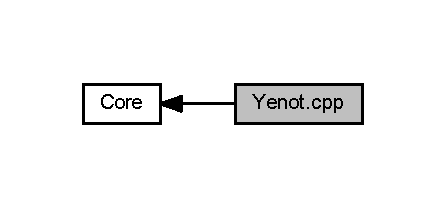
\includegraphics[width=214pt]{group__yenotcpp}
\end{center}
\end{figure}
\subsection*{Функции}
\begin{DoxyCompactItemize}
\item 
int \mbox{\hyperlink{group__yenotcpp_ga0ddf1224851353fc92bfbff6f499fa97}{main}} (int argc, char $\ast$argv\mbox{[}$\,$\mbox{]})
\end{DoxyCompactItemize}


\subsection{Подробное описание}


\subsection{Функции}
\mbox{\Hypertarget{group__yenotcpp_ga0ddf1224851353fc92bfbff6f499fa97}\label{group__yenotcpp_ga0ddf1224851353fc92bfbff6f499fa97}} 
\index{Yenot.\+cpp@{Yenot.\+cpp}!main@{main}}
\index{main@{main}!Yenot.\+cpp@{Yenot.\+cpp}}
\subsubsection{\texorpdfstring{main()}{main()}}
{\footnotesize\ttfamily int main (\begin{DoxyParamCaption}\item[{int}]{argc,  }\item[{char $\ast$}]{argv\mbox{[}$\,$\mbox{]} }\end{DoxyParamCaption})}



См. определение в файле Yenot.\+cpp строка 24


\hypertarget{group__yenot}{}\section{Yenot}
\label{group__yenot}\index{Yenot@{Yenot}}


Общие файлы  


Граф связей класса Yenot\+:\nopagebreak
\begin{figure}[H]
\begin{center}
\leavevmode
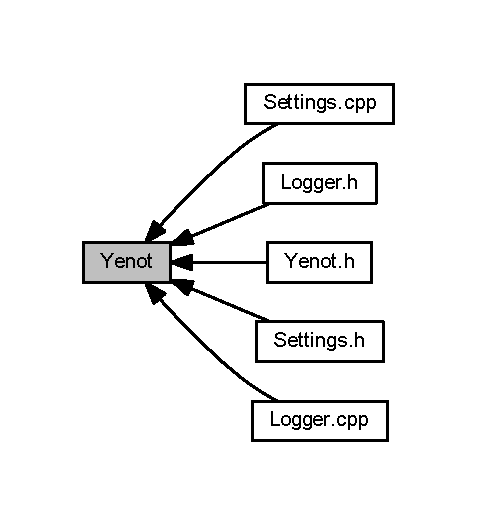
\includegraphics[width=229pt]{group__yenot}
\end{center}
\end{figure}
\subsection*{Группы}
\begin{DoxyCompactItemize}
\item 
\mbox{\hyperlink{group__loggercpp}{Logger.\+cpp}}
\item 
\mbox{\hyperlink{group__loggerh}{Logger.\+h}}
\item 
\mbox{\hyperlink{group__settingscpp}{Settings.\+cpp}}
\item 
\mbox{\hyperlink{group__settingsh}{Settings.\+h}}
\item 
\mbox{\hyperlink{group__yenoth}{Yenot.\+h}}
\end{DoxyCompactItemize}


\subsection{Подробное описание}
Общие файлы 


\hypertarget{group__core}{}\section{Core}
\label{group__core}\index{Core@{Core}}


Работа с изображениями, xml(yaml) файлами  


Граф связей класса Core\+:\nopagebreak
\begin{figure}[H]
\begin{center}
\leavevmode
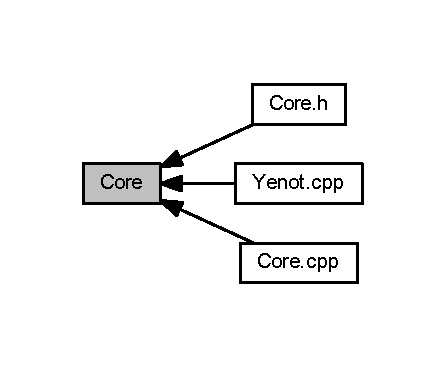
\includegraphics[width=214pt]{group__core}
\end{center}
\end{figure}
\subsection*{Группы}
\begin{DoxyCompactItemize}
\item 
\mbox{\hyperlink{group__corecpp}{Core.\+cpp}}
\item 
\mbox{\hyperlink{group__coreh}{Core.\+h}}
\item 
\mbox{\hyperlink{group__yenotcpp}{Yenot.\+cpp}}
\end{DoxyCompactItemize}


\subsection{Подробное описание}
Работа с изображениями, xml(yaml) файлами 


\hypertarget{group__test}{}\section{Test}
\label{group__test}\index{Test@{Test}}


Модуль тестирвания  


Граф связей класса Test\+:
\nopagebreak
\begin{figure}[H]
\begin{center}
\leavevmode
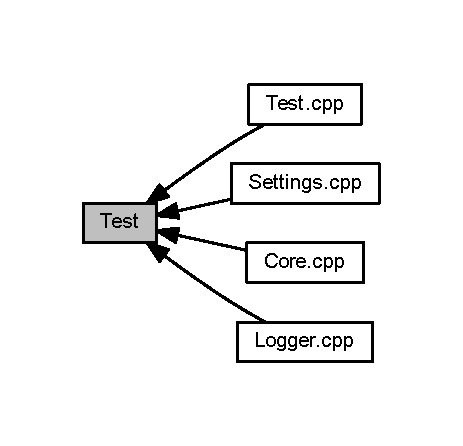
\includegraphics[width=222pt]{group__test}
\end{center}
\end{figure}
\subsection*{Группы}
\begin{DoxyCompactItemize}
\item 
\mbox{\hyperlink{group__corecpp}{Core.\+cpp}}
\item 
\mbox{\hyperlink{group__loggercpp}{Logger.\+cpp}}
\item 
\mbox{\hyperlink{group__settingscpp}{Settings.\+cpp}}
\item 
\mbox{\hyperlink{group__testcpp}{Test.\+cpp}}
\end{DoxyCompactItemize}


\subsection{Подробное описание}
Модуль тестирвания 


\hypertarget{group__yenoth}{}\section{Yenot.\+h}
\label{group__yenoth}\index{Yenot.\+h@{Yenot.\+h}}
Граф связей класса Yenot.\+h\+:
\nopagebreak
\begin{figure}[H]
\begin{center}
\leavevmode
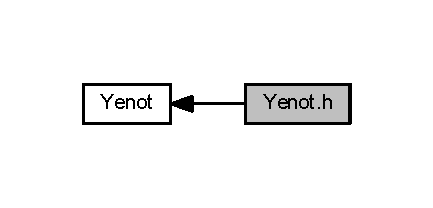
\includegraphics[width=208pt]{group__yenoth}
\end{center}
\end{figure}
\subsection*{Пространства имен}
\begin{DoxyCompactItemize}
\item 
 \mbox{\hyperlink{namespaceyenot}{yenot}}
\begin{DoxyCompactList}\small\item\em Пространство имён с константами \end{DoxyCompactList}\end{DoxyCompactItemize}


\subsection{Подробное описание}

\hypertarget{group__testcpp}{}\section{Test.\+cpp}
\label{group__testcpp}\index{Test.\+cpp@{Test.\+cpp}}
Граф связей класса Test.\+cpp\+:
\nopagebreak
\begin{figure}[H]
\begin{center}
\leavevmode
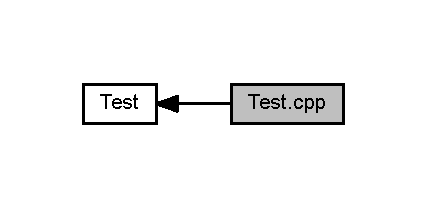
\includegraphics[width=205pt]{group__testcpp}
\end{center}
\end{figure}
\subsection*{Функции}
\begin{DoxyCompactItemize}
\item 
\mbox{\hyperlink{group__testcpp_ga0c6e823009aa80ab758989270ff8eec2}{T\+E\+ST}} (yenot\+\_\+test, correct\+\_\+connection\+\_\+testing\+\_\+module)
\end{DoxyCompactItemize}


\subsection{Подробное описание}


\subsection{Функции}
\mbox{\Hypertarget{group__testcpp_ga0c6e823009aa80ab758989270ff8eec2}\label{group__testcpp_ga0c6e823009aa80ab758989270ff8eec2}} 
\index{Test.\+cpp@{Test.\+cpp}!T\+E\+ST@{T\+E\+ST}}
\index{T\+E\+ST@{T\+E\+ST}!Test.\+cpp@{Test.\+cpp}}
\subsubsection{\texorpdfstring{T\+E\+S\+T()}{TEST()}}
{\footnotesize\ttfamily T\+E\+ST (\begin{DoxyParamCaption}\item[{yenot\+\_\+test}]{,  }\item[{correct\+\_\+connection\+\_\+testing\+\_\+module}]{ }\end{DoxyParamCaption})}



См. определение в файле Test.\+cpp строка 18


\chapter{Пространства имен}
\hypertarget{namespaceyenot}{}\section{Пространство имен yenot}
\label{namespaceyenot}\index{yenot@{yenot}}


Пространство имён с константами  


\subsection*{Переменные}
\begin{DoxyCompactItemize}
\item 
const char \mbox{\hyperlink{namespaceyenot_a376e7adfbabcae01c8305ed17d47d576}{F\+I\+L\+E\+\_\+\+N\+A\+M\+E\+\_\+\+C\+O\+N\+F\+IG}} \mbox{[}$\,$\mbox{]} = \char`\"{}./config.\+ini\char`\"{}
\begin{DoxyCompactList}\small\item\em Файл с настройками \end{DoxyCompactList}\item 
const char \mbox{\hyperlink{namespaceyenot_a6fdda6751433c679b7976669aff150b8}{F\+I\+L\+E\+\_\+\+N\+A\+M\+E\+\_\+\+L\+O\+G\+G\+ER}} \mbox{[}$\,$\mbox{]} = \char`\"{}Yenot.\+log\char`\"{}
\begin{DoxyCompactList}\small\item\em Файл с логами \end{DoxyCompactList}\item 
const char \mbox{\hyperlink{namespaceyenot_ae254e34a07790b92c8085e559be10f38}{F\+I\+L\+E\+\_\+\+N\+A\+M\+E\+\_\+\+D\+A\+T\+A\+B\+A\+SE}} \mbox{[}$\,$\mbox{]} = \char`\"{}database.\+xml\char`\"{}
\begin{DoxyCompactList}\small\item\em Файл, в котором хранятся \end{DoxyCompactList}\item 
const char \mbox{\hyperlink{namespaceyenot_af2253e95acd84452c01f492019f814f0}{N\+A\+M\+E\+\_\+\+D\+A\+T\+A\+B\+A\+SE}} \mbox{[}$\,$\mbox{]} = \char`\"{}database\char`\"{}
\item 
const char \mbox{\hyperlink{namespaceyenot_aa5230dc84adb2ca08b014531f83cd3c9}{E\+X\+T\+E\+N\+S\+I\+O\+N\+S\+\_\+\+D\+A\+T\+A\+B\+A\+S\+E\+\_\+\+M\+E\+M\+B\+ER}} \mbox{[}$\,$\mbox{]} = \char`\"{}.xml\char`\"{}
\item 
const char \mbox{\hyperlink{namespaceyenot_abf6ea7d0c605b7432754b26575046d32}{E\+X\+T\+E\+N\+S\+I\+O\+N\+S\+\_\+\+D\+A\+T\+A\+B\+A\+S\+E\+\_\+\+M\+E\+M\+B\+E\+R\+\_\+photo}} \mbox{[}$\,$\mbox{]} = \char`\"{}.png\char`\"{}
\item 
const int \mbox{\hyperlink{namespaceyenot_a08846c7b8addedd4db68b5cf3721bda1}{B\+U\+F\+F\+E\+R\+\_\+\+S\+I\+ZE}} = 128
\begin{DoxyCompactList}\small\item\em Стандартный размер буфера \end{DoxyCompactList}\item 
const char \mbox{\hyperlink{namespaceyenot_a2172a9f506029215b790a51a4023e1ac}{B\+L\+O\+C\+K\+\_\+\+C\+O\+RE}} \mbox{[}$\,$\mbox{]} = \char`\"{}Core\char`\"{}
\item 
const char \mbox{\hyperlink{namespaceyenot_a254a74c9007fa3d541605ff059a74add}{S\+E\+T\+T\+I\+N\+G\+S\+\_\+\+F\+A\+S\+T\+M\+O\+DE}} \mbox{[}$\,$\mbox{]} = \char`\"{}f\+Mode\char`\"{}
\item 
const char \mbox{\hyperlink{namespaceyenot_a7afad42fc42152730906aa57ef688c9a}{S\+E\+T\+T\+I\+N\+G\+S\+\_\+\+F\+A\+S\+T\+M\+O\+D\+E\+\_\+\+V\+A\+L\+UE}} \mbox{[}$\,$\mbox{]} = \char`\"{}0\char`\"{}
\item 
const int \mbox{\hyperlink{namespaceyenot_aef79e343f25022f42e779be319348eec}{S\+E\+T\+T\+I\+N\+G\+S\+\_\+\+F\+A\+S\+T\+M\+O\+D\+E\+\_\+\+V\+A\+L\+U\+E\+\_\+\+I\+NT}} = 0
\item 
const char \mbox{\hyperlink{namespaceyenot_a01aebb6f9dc4632eabd3ef606f5c75fb}{S\+E\+T\+T\+I\+N\+G\+S\+\_\+\+N\+O\+I\+S\+E\+\_\+\+R\+E\+D\+U\+C\+T\+I\+ON}} \mbox{[}$\,$\mbox{]} = \char`\"{}n\+Reduction\char`\"{}
\item 
const char \mbox{\hyperlink{namespaceyenot_a557e3ad9f3290543eed07f92644f1e33}{S\+E\+T\+T\+I\+N\+G\+S\+\_\+\+N\+O\+I\+S\+E\+\_\+\+R\+E\+D\+U\+C\+T\+I\+O\+N\+\_\+\+V\+A\+L\+UE}} \mbox{[}$\,$\mbox{]} = \char`\"{}1\char`\"{}
\item 
const int \mbox{\hyperlink{namespaceyenot_aaaef89f90413ee7a52a64d043e068136}{S\+E\+T\+T\+I\+N\+G\+S\+\_\+\+N\+O\+I\+S\+E\+\_\+\+R\+E\+D\+U\+C\+T\+I\+O\+N\+\_\+\+V\+A\+L\+U\+E\+\_\+\+I\+NT}} = 1
\item 
const char \mbox{\hyperlink{namespaceyenot_a6d4d3d03406bad7102e67e0f0d81edc2}{S\+E\+T\+T\+I\+N\+G\+S\+\_\+\+L\+I\+N\+E\+\_\+\+D\+E\+T\+E\+C\+T\+I\+ON}} \mbox{[}$\,$\mbox{]} = \char`\"{}l\+Detection\char`\"{}
\item 
const char \mbox{\hyperlink{namespaceyenot_ae8e9b52935a937554723960a8933df49}{S\+E\+T\+T\+I\+N\+G\+S\+\_\+\+L\+I\+N\+E\+\_\+\+D\+E\+T\+E\+C\+T\+I\+O\+N\+\_\+\+V\+A\+L\+UE}} \mbox{[}$\,$\mbox{]} = \char`\"{}1\char`\"{}
\item 
const int \mbox{\hyperlink{namespaceyenot_a07cb3f48df07dea977024678d96871f8}{S\+E\+T\+T\+I\+N\+G\+S\+\_\+\+L\+I\+N\+E\+\_\+\+D\+E\+T\+E\+C\+T\+I\+O\+N\+\_\+\+V\+A\+L\+U\+E\+\_\+\+I\+NT}} = 1
\item 
const char \mbox{\hyperlink{namespaceyenot_a6a7294929420d7790b72f733c98bcf56}{S\+E\+T\+T\+I\+N\+G\+S\+\_\+\+D\+E\+T\+E\+C\+T\+I\+ON}} \mbox{[}$\,$\mbox{]} = \char`\"{}detection\char`\"{}
\item 
const char \mbox{\hyperlink{namespaceyenot_a7d631c2848347b1df2d133225075ced0}{S\+E\+T\+T\+I\+N\+G\+S\+\_\+\+D\+E\+T\+E\+C\+T\+I\+O\+N\+\_\+\+V\+A\+L\+UE}} \mbox{[}$\,$\mbox{]} = \char`\"{}1\char`\"{}
\item 
const int \mbox{\hyperlink{namespaceyenot_a3043cfcdd8cc01993a692d71244049f6}{S\+E\+T\+T\+I\+N\+G\+S\+\_\+\+D\+E\+T\+E\+C\+T\+I\+O\+N\+\_\+\+V\+A\+L\+U\+E\+\_\+\+I\+NT}} = 1
\item 
const char \mbox{\hyperlink{namespaceyenot_a68308c1bd5623fffdc0992da59a687b3}{S\+E\+T\+T\+I\+N\+G\+S\+\_\+\+S\+A\+V\+E\+\_\+\+P\+R\+O\+C\+E\+S\+S\+E\+D\+\_\+\+I\+M\+A\+GE}} \mbox{[}$\,$\mbox{]} = \char`\"{}s\+Image\char`\"{}
\item 
const char \mbox{\hyperlink{namespaceyenot_a2e3ae4b394042b1c4cbc4ae56a4af012}{S\+E\+T\+T\+I\+N\+G\+S\+\_\+\+S\+A\+V\+E\+\_\+\+P\+R\+O\+C\+E\+S\+S\+E\+D\+\_\+\+I\+M\+A\+G\+E\+\_\+\+V\+A\+L\+UE}} \mbox{[}$\,$\mbox{]} = \char`\"{}0\char`\"{}
\item 
const int \mbox{\hyperlink{namespaceyenot_a58502c9277df0f0d680ddc344e5cea3e}{S\+E\+T\+T\+I\+N\+G\+S\+\_\+\+S\+A\+V\+E\+\_\+\+P\+R\+O\+C\+E\+S\+S\+E\+D\+\_\+\+I\+M\+A\+G\+E\+\_\+\+V\+A\+L\+U\+E\+\_\+\+I\+NT}} = 0
\item 
const char \mbox{\hyperlink{namespaceyenot_a6703c9900f97a42185c36c74c4147be3}{S\+E\+T\+T\+I\+N\+G\+S\+\_\+\+S\+A\+V\+E\+\_\+\+P\+R\+O\+C\+E\+S\+S\+E\+D\+\_\+\+I\+M\+A\+G\+E\+\_\+\+N\+A\+ME}} \mbox{[}$\,$\mbox{]} = \char`\"{}test.\+png\char`\"{}
\item 
const char \mbox{\hyperlink{namespaceyenot_a353e320b6fbef3dc210fd42ad10ff83c}{S\+E\+T\+T\+I\+N\+G\+S\+\_\+\+L\+OG}} \mbox{[}$\,$\mbox{]} = \char`\"{}log\char`\"{}
\item 
const char \mbox{\hyperlink{namespaceyenot_ab2eea8a981ab7baa7755cc64508671a0}{S\+E\+T\+T\+I\+N\+G\+S\+\_\+\+L\+O\+G\+\_\+\+V\+A\+L\+UE}} \mbox{[}$\,$\mbox{]} = \char`\"{}1\char`\"{}
\item 
const int \mbox{\hyperlink{namespaceyenot_ab756a3a6fb449bd27e6674cdf402b4d1}{S\+E\+T\+T\+I\+N\+G\+S\+\_\+\+L\+O\+G\+\_\+\+V\+A\+L\+U\+E\+\_\+\+I\+NT}} = 1
\item 
const char \mbox{\hyperlink{namespaceyenot_a420dc7e6e8223c7cd5ec7127995d46a0}{S\+E\+T\+T\+I\+N\+G\+S\+\_\+\+L\+O\+G\+\_\+\+T\+I\+ME}} \mbox{[}$\,$\mbox{]} = \char`\"{}l\+Time\char`\"{}
\item 
const char \mbox{\hyperlink{namespaceyenot_ae00932245c3089d385ef8ee3463df8ca}{S\+E\+T\+T\+I\+N\+G\+S\+\_\+\+L\+O\+G\+\_\+\+T\+I\+M\+E\+\_\+\+V\+A\+L\+UE}} \mbox{[}$\,$\mbox{]} = \char`\"{}1\char`\"{}
\item 
const int \mbox{\hyperlink{namespaceyenot_abc8b052e7f097163709fa71c4da4478d}{S\+E\+T\+T\+I\+N\+G\+S\+\_\+\+L\+O\+G\+\_\+\+T\+I\+M\+E\+\_\+\+V\+A\+L\+U\+E\+\_\+\+I\+NT}} = 1
\item 
const char \mbox{\hyperlink{namespaceyenot_a347fa05f62ae28e55301db755cf26210}{S\+E\+T\+T\+I\+N\+G\+S\+\_\+\+T\+E\+M\+P\+L\+A\+T\+E\+\_\+\+S\+I\+ZE}} \mbox{[}$\,$\mbox{]} = \char`\"{}templatesize\char`\"{}
\item 
const char \mbox{\hyperlink{namespaceyenot_acfc97705229a010013bb0433327bf707}{T\+E\+M\+P\+L\+A\+T\+E\+\_\+\+S\+I\+Z\+E\+\_\+\+S\+TR}} \mbox{[}$\,$\mbox{]} = \char`\"{}20\char`\"{}
\item 
const int \mbox{\hyperlink{namespaceyenot_a6c04317b4747d569efcf92266bb1051b}{T\+E\+M\+P\+L\+A\+T\+E\+\_\+\+S\+I\+ZE}} = 20
\item 
const char \mbox{\hyperlink{namespaceyenot_a6a132f52235e5b9454c850b4f5343ce3}{S\+E\+T\+T\+I\+N\+G\+S\+\_\+\+S\+I\+Z\+E\+\_\+\+P\+H\+O\+TO}} \mbox{[}$\,$\mbox{]} = \char`\"{}size\+Photo\char`\"{}
\item 
const char \mbox{\hyperlink{namespaceyenot_a172f1253ba2c664d26caffab97a6253d}{S\+I\+Z\+E\+\_\+\+P\+H\+O\+T\+O\+\_\+\+S\+TR}} \mbox{[}$\,$\mbox{]} = \char`\"{}512\char`\"{}
\item 
const int \mbox{\hyperlink{namespaceyenot_a501462c649059c5efe3019823a607670}{S\+I\+Z\+E\+\_\+\+P\+H\+O\+TO}} = 512
\item 
const int \mbox{\hyperlink{namespaceyenot_ad85720cad8409ab5ef5cc47afc84645c}{D\+I\+A\+M\+E\+T\+E\+R\+\_\+\+E\+A\+C\+H\+\_\+\+P\+I\+X\+EL}} = 9
\item 
const int \mbox{\hyperlink{namespaceyenot_affd7404833d15c98fbd85249f43f98da}{S\+I\+G\+M\+A\+\_\+\+C\+O\+L\+OR}} = 75
\item 
const int \mbox{\hyperlink{namespaceyenot_ad45191f613b95ca3398e6eab5e202406}{S\+I\+G\+M\+A\+\_\+\+S\+P\+A\+CE}} = 75
\item 
const int \mbox{\hyperlink{namespaceyenot_aa753d0e3e99fb4b37b3930996bdfe563}{K\+E\+R\+N\+E\+L\+\_\+X}} = 5
\item 
const int \mbox{\hyperlink{namespaceyenot_a33a5af73a30e2b5684ee02cc4bf4c374}{K\+E\+R\+N\+E\+L\+\_\+Y}} = 5
\item 
const char \mbox{\hyperlink{namespaceyenot_a73be0cdcde2af378cd4043f56d4776e2}{B\+L\+O\+C\+K\+\_\+\+L\+O\+G\+G\+ER}} \mbox{[}$\,$\mbox{]} = \char`\"{}Logger\char`\"{}
\item 
const char \mbox{\hyperlink{namespaceyenot_a1133c576c0c3eebe5aa6c43529a56f21}{L\+O\+G\+G\+E\+R\+\_\+\+L\+E\+V\+E\+L\+\_\+\+W\+A\+R\+N\+I\+NG}} \mbox{[}$\,$\mbox{]} = \char`\"{}W\+A\+RN\char`\"{}
\begin{DoxyCompactList}\small\item\em Уровень предупреждения \end{DoxyCompactList}\item 
const char \mbox{\hyperlink{namespaceyenot_a08c0d88b074bcba3b7d79d019211a1ac}{L\+O\+G\+G\+E\+R\+\_\+\+L\+E\+V\+E\+L\+\_\+\+E\+R\+R\+OR}} \mbox{[}$\,$\mbox{]} = \char`\"{}E\+R\+R\+OR\char`\"{}
\begin{DoxyCompactList}\small\item\em Уровень ошибки \end{DoxyCompactList}\item 
const char \mbox{\hyperlink{namespaceyenot_a75d435531623705520a8bd478ae6e3ed}{L\+O\+G\+G\+E\+R\+\_\+\+L\+E\+V\+E\+L\+\_\+\+M\+E\+S\+S\+A\+GE}} \mbox{[}$\,$\mbox{]} = \char`\"{}M\+SG\char`\"{}
\begin{DoxyCompactList}\small\item\em Уровень сообщение \end{DoxyCompactList}\item 
const char \mbox{\hyperlink{namespaceyenot_ae3c6bd195ef1c9bdcbd48e5b44e17aaf}{L\+O\+G\+G\+E\+R\+\_\+\+M\+E\+S\+S\+A\+G\+E\+\_\+\+N\+O\+I\+S\+E\+\_\+\+R\+E\+M\+O\+V\+AL}} \mbox{[}$\,$\mbox{]} = \char`\"{}Noise filter is disabled.\char`\"{}
\begin{DoxyCompactList}\small\item\em Сообщение в лог о том, что фильтр шума отключен \end{DoxyCompactList}\item 
const char \mbox{\hyperlink{namespaceyenot_a3cc24a045a30435ab78be6014ff26a16}{L\+O\+G\+G\+E\+R\+\_\+\+M\+E\+S\+S\+A\+G\+E\+\_\+\+L\+I\+N\+E\+\_\+\+D\+E\+T\+E\+C\+T\+I\+ON}} \mbox{[}$\,$\mbox{]} = \char`\"{}Line \mbox{\hyperlink{group__coreh_ga0ef39a5ada0921b3abf8906957746b86}{detection}} is disabled.\char`\"{}
\begin{DoxyCompactList}\small\item\em Сообщение в лог о том, что детектор границ отключен \end{DoxyCompactList}\item 
const char \mbox{\hyperlink{namespaceyenot_a23d265aa1784a96ebe7ce76bedd308a6}{L\+O\+G\+G\+E\+R\+\_\+\+M\+E\+S\+S\+A\+G\+E\+\_\+\+F\+A\+S\+T\+\_\+\+M\+O\+DE}} \mbox{[}$\,$\mbox{]} = \char`\"{}Fast mode enabled.\char`\"{}
\begin{DoxyCompactList}\small\item\em Сообщение в лог о том, что быстрый режим включен \end{DoxyCompactList}\item 
const char \mbox{\hyperlink{namespaceyenot_ace626bb1b7477b39cf2864aa0d0924e9}{L\+O\+G\+G\+E\+R\+\_\+\+M\+E\+S\+S\+A\+G\+E\+\_\+\+C\+R\+E\+A\+T\+E\+\_\+\+D\+IR}} \mbox{[}$\,$\mbox{]} = \char`\"{}Folder created.\char`\"{}
\begin{DoxyCompactList}\small\item\em Сообщение в лог о том, что папка создана \end{DoxyCompactList}\item 
const char \mbox{\hyperlink{namespaceyenot_ae73ee066dad5c6455cb406ab3aa0473f}{L\+O\+G\+G\+E\+R\+\_\+\+M\+E\+S\+S\+A\+G\+E\+\_\+\+C\+R\+E\+A\+T\+E\+\_\+\+D\+I\+R\+\_\+\+N\+OT}} \mbox{[}$\,$\mbox{]} = \char`\"{}Folder creation failed.\char`\"{}
\begin{DoxyCompactList}\small\item\em Сообщение в лог о том, что не удалось создать папку \end{DoxyCompactList}\item 
const int \mbox{\hyperlink{namespaceyenot_a8206ed93e65c9e89395c2823a5f18786}{E\+R\+R\+O\+R\+\_\+\+I\+N\+IT}} = -\/100
\begin{DoxyCompactList}\small\item\em Ошибка инициализации \end{DoxyCompactList}\item 
const int \mbox{\hyperlink{namespaceyenot_a3c1c146cfa3fc68ce0e1950b93270849}{E\+R\+R\+O\+R\+\_\+\+I\+M\+A\+GE}} = -\/200
\begin{DoxyCompactList}\small\item\em Ошибка связанная с входным изображением. Возможно не достаточно аргументов \end{DoxyCompactList}\item 
const int \mbox{\hyperlink{namespaceyenot_a9b11e5890ebee4b3ace81f058483b7af}{E\+R\+R\+O\+R\+\_\+\+C\+L\+E\+A\+R\+N\+I\+NG}} = -\/300
\begin{DoxyCompactList}\small\item\em Ошибка связанная с очисткой дубликатов \end{DoxyCompactList}\item 
const int \mbox{\hyperlink{namespaceyenot_a787166b1304265d12d6ff10b175a66bc}{E\+R\+R\+O\+R\+\_\+\+R\+E\+S\+I\+ZE}} = -\/400
\begin{DoxyCompactList}\small\item\em Ошибка связанная с изменением размера фотографии \end{DoxyCompactList}\item 
const int \mbox{\hyperlink{namespaceyenot_a0699d20f9a904f7faf8b63cc7fc31c63}{E\+R\+R\+O\+R\+\_\+\+N\+O\+I\+S\+E\+\_\+\+R\+E\+M\+O\+V\+AL}} = -\/500
\begin{DoxyCompactList}\small\item\em Ошибка связанная с фильтвом шума \end{DoxyCompactList}\item 
const int \mbox{\hyperlink{namespaceyenot_ab63291c5dfdea5865dc7a32401095215}{E\+R\+R\+O\+R\+\_\+\+L\+I\+N\+E\+\_\+\+D\+E\+T\+E\+C\+T\+I\+ON}} = -\/600
\begin{DoxyCompactList}\small\item\em Ошибка связанная с детектором границ \end{DoxyCompactList}\item 
const int \mbox{\hyperlink{namespaceyenot_af6dc289a999d852dd3da0134f47cda0f}{E\+R\+R\+O\+R\+\_\+\+D\+E\+T\+E\+C\+T\+I\+ON}} = -\/700
\begin{DoxyCompactList}\small\item\em Ошибка \end{DoxyCompactList}\item 
const int \mbox{\hyperlink{namespaceyenot_a34fbed9d403672deb1f0f73139f26ee6}{E\+R\+R\+O\+R\+\_\+\+D\+A\+T\+A\+B\+A\+SE}} = -\/800
\begin{DoxyCompactList}\small\item\em Ошибка в модуле распознавания логотипов \end{DoxyCompactList}\item 
const char \mbox{\hyperlink{namespaceyenot_af958287fcf5b41e632a87bd1a795c74b}{E\+R\+R\+O\+R\+\_\+\+I\+N\+I\+T\+\_\+\+D\+A\+T\+A\+B\+A\+S\+E\+\_\+\+A\+DD}} \mbox{[}$\,$\mbox{]} = \char`\"{}The file name can not be empty.\char`\"{}
\begin{DoxyCompactList}\small\item\em Сообщение в лог о том, что название файла с каскадом не может быть пустым \end{DoxyCompactList}\item 
const char \mbox{\hyperlink{namespaceyenot_adec37b1319feb436842ed87c9741df97}{E\+R\+R\+O\+R\+\_\+\+D\+A\+T\+A\+B\+A\+S\+E\+\_\+\+A\+D\+D\+\_\+\+A\+R\+G\+U\+M\+E\+N\+TS}} \mbox{[}$\,$\mbox{]} = \char`\"{}Few arguments\char`\"{}
\begin{DoxyCompactList}\small\item\em Сообщение в лог о том, что не достаточно аргументов для запуска программы \end{DoxyCompactList}\item 
const char \mbox{\hyperlink{namespaceyenot_abc55bd8e208d61e4d5055b305d998624}{B\+L\+O\+C\+K\+\_\+\+D\+E\+S\+C\+R\+I\+P\+T\+I\+ON}} \mbox{[}$\,$\mbox{]} = \char`\"{}description\char`\"{}
\item 
const char \mbox{\hyperlink{namespaceyenot_a15f1fcc1f696f7e59aaf534d28eeebb9}{C\+A\+R\+\_\+\+M\+O\+D\+E\+L\+\_\+\+E\+X\+A\+M\+P\+L\+E\+\_\+\+D\+E\+S\+C\+R\+I\+P\+T\+I\+ON}} \mbox{[}$\,$\mbox{]} = \char`\"{}Brand\+: \textbackslash{}\char`\"{}Example\textbackslash{}\char`\"{}\char`\"{}
\begin{DoxyCompactList}\small\item\em Пример описания логотипа \end{DoxyCompactList}\item 
const char \mbox{\hyperlink{namespaceyenot_ad659efb70fd572b82d45f7ec0d9e7ff3}{C\+A\+R\+\_\+\+M\+O\+D\+E\+L\+\_\+\+E\+X\+A\+M\+P\+L\+E\+\_\+\+F\+I\+LE}} \mbox{[}$\,$\mbox{]} = \char`\"{}example.\+xml\char`\"{}
\begin{DoxyCompactList}\small\item\em Пример файла с каскадом \end{DoxyCompactList}\item 
const char \mbox{\hyperlink{namespaceyenot_abc01a4ee833e7c083cba257351b21769}{D\+E\+S\+C\+R\+I\+P\+T\+I\+O\+N\+\_\+\+N\+O\+T\+\_\+\+F\+O\+U\+ND}} \mbox{[}$\,$\mbox{]} = \char`\"{}The brand name is not set\char`\"{}
\begin{DoxyCompactList}\small\item\em Сообщение о том, что для данного логотипа нет описания \end{DoxyCompactList}\end{DoxyCompactItemize}


\subsection{Подробное описание}
Пространство имён с константами 

General -\/ Основные константы

Core -\/ Ядро

Filters -\/ Фильтры

Logger -\/ Модуль логирования

Log messages -\/ Сообщения для вывода в логами

Errors -\/ Ошибки

Car model -\/ Пример 

\subsection{Переменные}
\mbox{\Hypertarget{namespaceyenot_a2172a9f506029215b790a51a4023e1ac}\label{namespaceyenot_a2172a9f506029215b790a51a4023e1ac}} 
\index{yenot@{yenot}!B\+L\+O\+C\+K\+\_\+\+C\+O\+RE@{B\+L\+O\+C\+K\+\_\+\+C\+O\+RE}}
\index{B\+L\+O\+C\+K\+\_\+\+C\+O\+RE@{B\+L\+O\+C\+K\+\_\+\+C\+O\+RE}!yenot@{yenot}}
\subsubsection{\texorpdfstring{B\+L\+O\+C\+K\+\_\+\+C\+O\+RE}{BLOCK\_CORE}}
{\footnotesize\ttfamily const char yenot\+::\+B\+L\+O\+C\+K\+\_\+\+C\+O\+RE\mbox{[}$\,$\mbox{]} = \char`\"{}Core\char`\"{}}

Блок настроек ядра.

ini файл 
\begin{DoxyCode}
[Core]
...
\end{DoxyCode}
 

См. определение в файле Yenot.\+h строка 85

\mbox{\Hypertarget{namespaceyenot_abc55bd8e208d61e4d5055b305d998624}\label{namespaceyenot_abc55bd8e208d61e4d5055b305d998624}} 
\index{yenot@{yenot}!B\+L\+O\+C\+K\+\_\+\+D\+E\+S\+C\+R\+I\+P\+T\+I\+ON@{B\+L\+O\+C\+K\+\_\+\+D\+E\+S\+C\+R\+I\+P\+T\+I\+ON}}
\index{B\+L\+O\+C\+K\+\_\+\+D\+E\+S\+C\+R\+I\+P\+T\+I\+ON@{B\+L\+O\+C\+K\+\_\+\+D\+E\+S\+C\+R\+I\+P\+T\+I\+ON}!yenot@{yenot}}
\subsubsection{\texorpdfstring{B\+L\+O\+C\+K\+\_\+\+D\+E\+S\+C\+R\+I\+P\+T\+I\+ON}{BLOCK\_DESCRIPTION}}
{\footnotesize\ttfamily const char yenot\+::\+B\+L\+O\+C\+K\+\_\+\+D\+E\+S\+C\+R\+I\+P\+T\+I\+ON\mbox{[}$\,$\mbox{]} = \char`\"{}description\char`\"{}}

Блок модуля поиска описания логотипа

ini файл 
\begin{DoxyCode}
[\mbox{\hyperlink{group__corecpp_gaa85ae460901348b74381239ce0517d5f}{description}}]
...
\end{DoxyCode}
 

См. определение в файле Yenot.\+h строка 328

\mbox{\Hypertarget{namespaceyenot_a73be0cdcde2af378cd4043f56d4776e2}\label{namespaceyenot_a73be0cdcde2af378cd4043f56d4776e2}} 
\index{yenot@{yenot}!B\+L\+O\+C\+K\+\_\+\+L\+O\+G\+G\+ER@{B\+L\+O\+C\+K\+\_\+\+L\+O\+G\+G\+ER}}
\index{B\+L\+O\+C\+K\+\_\+\+L\+O\+G\+G\+ER@{B\+L\+O\+C\+K\+\_\+\+L\+O\+G\+G\+ER}!yenot@{yenot}}
\subsubsection{\texorpdfstring{B\+L\+O\+C\+K\+\_\+\+L\+O\+G\+G\+ER}{BLOCK\_LOGGER}}
{\footnotesize\ttfamily const char yenot\+::\+B\+L\+O\+C\+K\+\_\+\+L\+O\+G\+G\+ER\mbox{[}$\,$\mbox{]} = \char`\"{}Logger\char`\"{}}

Блок модуля логирования.

ini файл 
\begin{DoxyCode}
[Logger]
...
\end{DoxyCode}
 

См. определение в файле Yenot.\+h строка 253

\mbox{\Hypertarget{namespaceyenot_a08846c7b8addedd4db68b5cf3721bda1}\label{namespaceyenot_a08846c7b8addedd4db68b5cf3721bda1}} 
\index{yenot@{yenot}!B\+U\+F\+F\+E\+R\+\_\+\+S\+I\+ZE@{B\+U\+F\+F\+E\+R\+\_\+\+S\+I\+ZE}}
\index{B\+U\+F\+F\+E\+R\+\_\+\+S\+I\+ZE@{B\+U\+F\+F\+E\+R\+\_\+\+S\+I\+ZE}!yenot@{yenot}}
\subsubsection{\texorpdfstring{B\+U\+F\+F\+E\+R\+\_\+\+S\+I\+ZE}{BUFFER\_SIZE}}
{\footnotesize\ttfamily const int yenot\+::\+B\+U\+F\+F\+E\+R\+\_\+\+S\+I\+ZE = 128}



Стандартный размер буфера 



См. определение в файле Yenot.\+h строка 72

\mbox{\Hypertarget{namespaceyenot_a15f1fcc1f696f7e59aaf534d28eeebb9}\label{namespaceyenot_a15f1fcc1f696f7e59aaf534d28eeebb9}} 
\index{yenot@{yenot}!C\+A\+R\+\_\+\+M\+O\+D\+E\+L\+\_\+\+E\+X\+A\+M\+P\+L\+E\+\_\+\+D\+E\+S\+C\+R\+I\+P\+T\+I\+ON@{C\+A\+R\+\_\+\+M\+O\+D\+E\+L\+\_\+\+E\+X\+A\+M\+P\+L\+E\+\_\+\+D\+E\+S\+C\+R\+I\+P\+T\+I\+ON}}
\index{C\+A\+R\+\_\+\+M\+O\+D\+E\+L\+\_\+\+E\+X\+A\+M\+P\+L\+E\+\_\+\+D\+E\+S\+C\+R\+I\+P\+T\+I\+ON@{C\+A\+R\+\_\+\+M\+O\+D\+E\+L\+\_\+\+E\+X\+A\+M\+P\+L\+E\+\_\+\+D\+E\+S\+C\+R\+I\+P\+T\+I\+ON}!yenot@{yenot}}
\subsubsection{\texorpdfstring{C\+A\+R\+\_\+\+M\+O\+D\+E\+L\+\_\+\+E\+X\+A\+M\+P\+L\+E\+\_\+\+D\+E\+S\+C\+R\+I\+P\+T\+I\+ON}{CAR\_MODEL\_EXAMPLE\_DESCRIPTION}}
{\footnotesize\ttfamily const char yenot\+::\+C\+A\+R\+\_\+\+M\+O\+D\+E\+L\+\_\+\+E\+X\+A\+M\+P\+L\+E\+\_\+\+D\+E\+S\+C\+R\+I\+P\+T\+I\+ON\mbox{[}$\,$\mbox{]} = \char`\"{}Brand\+: \textbackslash{}\char`\"{}Example\textbackslash{}\char`\"{}\char`\"{}}



Пример описания логотипа 



См. определение в файле Yenot.\+h строка 331

\mbox{\Hypertarget{namespaceyenot_ad659efb70fd572b82d45f7ec0d9e7ff3}\label{namespaceyenot_ad659efb70fd572b82d45f7ec0d9e7ff3}} 
\index{yenot@{yenot}!C\+A\+R\+\_\+\+M\+O\+D\+E\+L\+\_\+\+E\+X\+A\+M\+P\+L\+E\+\_\+\+F\+I\+LE@{C\+A\+R\+\_\+\+M\+O\+D\+E\+L\+\_\+\+E\+X\+A\+M\+P\+L\+E\+\_\+\+F\+I\+LE}}
\index{C\+A\+R\+\_\+\+M\+O\+D\+E\+L\+\_\+\+E\+X\+A\+M\+P\+L\+E\+\_\+\+F\+I\+LE@{C\+A\+R\+\_\+\+M\+O\+D\+E\+L\+\_\+\+E\+X\+A\+M\+P\+L\+E\+\_\+\+F\+I\+LE}!yenot@{yenot}}
\subsubsection{\texorpdfstring{C\+A\+R\+\_\+\+M\+O\+D\+E\+L\+\_\+\+E\+X\+A\+M\+P\+L\+E\+\_\+\+F\+I\+LE}{CAR\_MODEL\_EXAMPLE\_FILE}}
{\footnotesize\ttfamily const char yenot\+::\+C\+A\+R\+\_\+\+M\+O\+D\+E\+L\+\_\+\+E\+X\+A\+M\+P\+L\+E\+\_\+\+F\+I\+LE\mbox{[}$\,$\mbox{]} = \char`\"{}example.\+xml\char`\"{}}



Пример файла с каскадом 



См. определение в файле Yenot.\+h строка 334

\mbox{\Hypertarget{namespaceyenot_abc01a4ee833e7c083cba257351b21769}\label{namespaceyenot_abc01a4ee833e7c083cba257351b21769}} 
\index{yenot@{yenot}!D\+E\+S\+C\+R\+I\+P\+T\+I\+O\+N\+\_\+\+N\+O\+T\+\_\+\+F\+O\+U\+ND@{D\+E\+S\+C\+R\+I\+P\+T\+I\+O\+N\+\_\+\+N\+O\+T\+\_\+\+F\+O\+U\+ND}}
\index{D\+E\+S\+C\+R\+I\+P\+T\+I\+O\+N\+\_\+\+N\+O\+T\+\_\+\+F\+O\+U\+ND@{D\+E\+S\+C\+R\+I\+P\+T\+I\+O\+N\+\_\+\+N\+O\+T\+\_\+\+F\+O\+U\+ND}!yenot@{yenot}}
\subsubsection{\texorpdfstring{D\+E\+S\+C\+R\+I\+P\+T\+I\+O\+N\+\_\+\+N\+O\+T\+\_\+\+F\+O\+U\+ND}{DESCRIPTION\_NOT\_FOUND}}
{\footnotesize\ttfamily const char yenot\+::\+D\+E\+S\+C\+R\+I\+P\+T\+I\+O\+N\+\_\+\+N\+O\+T\+\_\+\+F\+O\+U\+ND\mbox{[}$\,$\mbox{]} = \char`\"{}The brand name is not set\char`\"{}}



Сообщение о том, что для данного логотипа нет описания 



См. определение в файле Yenot.\+h строка 337

\mbox{\Hypertarget{namespaceyenot_ad85720cad8409ab5ef5cc47afc84645c}\label{namespaceyenot_ad85720cad8409ab5ef5cc47afc84645c}} 
\index{yenot@{yenot}!D\+I\+A\+M\+E\+T\+E\+R\+\_\+\+E\+A\+C\+H\+\_\+\+P\+I\+X\+EL@{D\+I\+A\+M\+E\+T\+E\+R\+\_\+\+E\+A\+C\+H\+\_\+\+P\+I\+X\+EL}}
\index{D\+I\+A\+M\+E\+T\+E\+R\+\_\+\+E\+A\+C\+H\+\_\+\+P\+I\+X\+EL@{D\+I\+A\+M\+E\+T\+E\+R\+\_\+\+E\+A\+C\+H\+\_\+\+P\+I\+X\+EL}!yenot@{yenot}}
\subsubsection{\texorpdfstring{D\+I\+A\+M\+E\+T\+E\+R\+\_\+\+E\+A\+C\+H\+\_\+\+P\+I\+X\+EL}{DIAMETER\_EACH\_PIXEL}}
{\footnotesize\ttfamily const int yenot\+::\+D\+I\+A\+M\+E\+T\+E\+R\+\_\+\+E\+A\+C\+H\+\_\+\+P\+I\+X\+EL = 9}

Фильтр.

Диаметр каждого пикселя 

См. определение в файле Yenot.\+h строка 220

\mbox{\Hypertarget{namespaceyenot_a9b11e5890ebee4b3ace81f058483b7af}\label{namespaceyenot_a9b11e5890ebee4b3ace81f058483b7af}} 
\index{yenot@{yenot}!E\+R\+R\+O\+R\+\_\+\+C\+L\+E\+A\+R\+N\+I\+NG@{E\+R\+R\+O\+R\+\_\+\+C\+L\+E\+A\+R\+N\+I\+NG}}
\index{E\+R\+R\+O\+R\+\_\+\+C\+L\+E\+A\+R\+N\+I\+NG@{E\+R\+R\+O\+R\+\_\+\+C\+L\+E\+A\+R\+N\+I\+NG}!yenot@{yenot}}
\subsubsection{\texorpdfstring{E\+R\+R\+O\+R\+\_\+\+C\+L\+E\+A\+R\+N\+I\+NG}{ERROR\_CLEARNING}}
{\footnotesize\ttfamily const int yenot\+::\+E\+R\+R\+O\+R\+\_\+\+C\+L\+E\+A\+R\+N\+I\+NG = -\/300}



Ошибка связанная с очисткой дубликатов 



См. определение в файле Yenot.\+h строка 294

\mbox{\Hypertarget{namespaceyenot_a34fbed9d403672deb1f0f73139f26ee6}\label{namespaceyenot_a34fbed9d403672deb1f0f73139f26ee6}} 
\index{yenot@{yenot}!E\+R\+R\+O\+R\+\_\+\+D\+A\+T\+A\+B\+A\+SE@{E\+R\+R\+O\+R\+\_\+\+D\+A\+T\+A\+B\+A\+SE}}
\index{E\+R\+R\+O\+R\+\_\+\+D\+A\+T\+A\+B\+A\+SE@{E\+R\+R\+O\+R\+\_\+\+D\+A\+T\+A\+B\+A\+SE}!yenot@{yenot}}
\subsubsection{\texorpdfstring{E\+R\+R\+O\+R\+\_\+\+D\+A\+T\+A\+B\+A\+SE}{ERROR\_DATABASE}}
{\footnotesize\ttfamily const int yenot\+::\+E\+R\+R\+O\+R\+\_\+\+D\+A\+T\+A\+B\+A\+SE = -\/800}



Ошибка в модуле распознавания логотипов 



См. определение в файле Yenot.\+h строка 309

\mbox{\Hypertarget{namespaceyenot_adec37b1319feb436842ed87c9741df97}\label{namespaceyenot_adec37b1319feb436842ed87c9741df97}} 
\index{yenot@{yenot}!E\+R\+R\+O\+R\+\_\+\+D\+A\+T\+A\+B\+A\+S\+E\+\_\+\+A\+D\+D\+\_\+\+A\+R\+G\+U\+M\+E\+N\+TS@{E\+R\+R\+O\+R\+\_\+\+D\+A\+T\+A\+B\+A\+S\+E\+\_\+\+A\+D\+D\+\_\+\+A\+R\+G\+U\+M\+E\+N\+TS}}
\index{E\+R\+R\+O\+R\+\_\+\+D\+A\+T\+A\+B\+A\+S\+E\+\_\+\+A\+D\+D\+\_\+\+A\+R\+G\+U\+M\+E\+N\+TS@{E\+R\+R\+O\+R\+\_\+\+D\+A\+T\+A\+B\+A\+S\+E\+\_\+\+A\+D\+D\+\_\+\+A\+R\+G\+U\+M\+E\+N\+TS}!yenot@{yenot}}
\subsubsection{\texorpdfstring{E\+R\+R\+O\+R\+\_\+\+D\+A\+T\+A\+B\+A\+S\+E\+\_\+\+A\+D\+D\+\_\+\+A\+R\+G\+U\+M\+E\+N\+TS}{ERROR\_DATABASE\_ADD\_ARGUMENTS}}
{\footnotesize\ttfamily const char yenot\+::\+E\+R\+R\+O\+R\+\_\+\+D\+A\+T\+A\+B\+A\+S\+E\+\_\+\+A\+D\+D\+\_\+\+A\+R\+G\+U\+M\+E\+N\+TS\mbox{[}$\,$\mbox{]} = \char`\"{}Few arguments\char`\"{}}



Сообщение в лог о том, что не достаточно аргументов для запуска программы 



См. определение в файле Yenot.\+h строка 315

\mbox{\Hypertarget{namespaceyenot_af6dc289a999d852dd3da0134f47cda0f}\label{namespaceyenot_af6dc289a999d852dd3da0134f47cda0f}} 
\index{yenot@{yenot}!E\+R\+R\+O\+R\+\_\+\+D\+E\+T\+E\+C\+T\+I\+ON@{E\+R\+R\+O\+R\+\_\+\+D\+E\+T\+E\+C\+T\+I\+ON}}
\index{E\+R\+R\+O\+R\+\_\+\+D\+E\+T\+E\+C\+T\+I\+ON@{E\+R\+R\+O\+R\+\_\+\+D\+E\+T\+E\+C\+T\+I\+ON}!yenot@{yenot}}
\subsubsection{\texorpdfstring{E\+R\+R\+O\+R\+\_\+\+D\+E\+T\+E\+C\+T\+I\+ON}{ERROR\_DETECTION}}
{\footnotesize\ttfamily const int yenot\+::\+E\+R\+R\+O\+R\+\_\+\+D\+E\+T\+E\+C\+T\+I\+ON = -\/700}



Ошибка 



См. определение в файле Yenot.\+h строка 306

\mbox{\Hypertarget{namespaceyenot_a3c1c146cfa3fc68ce0e1950b93270849}\label{namespaceyenot_a3c1c146cfa3fc68ce0e1950b93270849}} 
\index{yenot@{yenot}!E\+R\+R\+O\+R\+\_\+\+I\+M\+A\+GE@{E\+R\+R\+O\+R\+\_\+\+I\+M\+A\+GE}}
\index{E\+R\+R\+O\+R\+\_\+\+I\+M\+A\+GE@{E\+R\+R\+O\+R\+\_\+\+I\+M\+A\+GE}!yenot@{yenot}}
\subsubsection{\texorpdfstring{E\+R\+R\+O\+R\+\_\+\+I\+M\+A\+GE}{ERROR\_IMAGE}}
{\footnotesize\ttfamily const int yenot\+::\+E\+R\+R\+O\+R\+\_\+\+I\+M\+A\+GE = -\/200}



Ошибка связанная с входным изображением. Возможно не достаточно аргументов 



См. определение в файле Yenot.\+h строка 291

\mbox{\Hypertarget{namespaceyenot_a8206ed93e65c9e89395c2823a5f18786}\label{namespaceyenot_a8206ed93e65c9e89395c2823a5f18786}} 
\index{yenot@{yenot}!E\+R\+R\+O\+R\+\_\+\+I\+N\+IT@{E\+R\+R\+O\+R\+\_\+\+I\+N\+IT}}
\index{E\+R\+R\+O\+R\+\_\+\+I\+N\+IT@{E\+R\+R\+O\+R\+\_\+\+I\+N\+IT}!yenot@{yenot}}
\subsubsection{\texorpdfstring{E\+R\+R\+O\+R\+\_\+\+I\+N\+IT}{ERROR\_INIT}}
{\footnotesize\ttfamily const int yenot\+::\+E\+R\+R\+O\+R\+\_\+\+I\+N\+IT = -\/100}



Ошибка инициализации 



См. определение в файле Yenot.\+h строка 288

\mbox{\Hypertarget{namespaceyenot_af958287fcf5b41e632a87bd1a795c74b}\label{namespaceyenot_af958287fcf5b41e632a87bd1a795c74b}} 
\index{yenot@{yenot}!E\+R\+R\+O\+R\+\_\+\+I\+N\+I\+T\+\_\+\+D\+A\+T\+A\+B\+A\+S\+E\+\_\+\+A\+DD@{E\+R\+R\+O\+R\+\_\+\+I\+N\+I\+T\+\_\+\+D\+A\+T\+A\+B\+A\+S\+E\+\_\+\+A\+DD}}
\index{E\+R\+R\+O\+R\+\_\+\+I\+N\+I\+T\+\_\+\+D\+A\+T\+A\+B\+A\+S\+E\+\_\+\+A\+DD@{E\+R\+R\+O\+R\+\_\+\+I\+N\+I\+T\+\_\+\+D\+A\+T\+A\+B\+A\+S\+E\+\_\+\+A\+DD}!yenot@{yenot}}
\subsubsection{\texorpdfstring{E\+R\+R\+O\+R\+\_\+\+I\+N\+I\+T\+\_\+\+D\+A\+T\+A\+B\+A\+S\+E\+\_\+\+A\+DD}{ERROR\_INIT\_DATABASE\_ADD}}
{\footnotesize\ttfamily const char yenot\+::\+E\+R\+R\+O\+R\+\_\+\+I\+N\+I\+T\+\_\+\+D\+A\+T\+A\+B\+A\+S\+E\+\_\+\+A\+DD\mbox{[}$\,$\mbox{]} = \char`\"{}The file name can not be empty.\char`\"{}}



Сообщение в лог о том, что название файла с каскадом не может быть пустым 



См. определение в файле Yenot.\+h строка 312

\mbox{\Hypertarget{namespaceyenot_ab63291c5dfdea5865dc7a32401095215}\label{namespaceyenot_ab63291c5dfdea5865dc7a32401095215}} 
\index{yenot@{yenot}!E\+R\+R\+O\+R\+\_\+\+L\+I\+N\+E\+\_\+\+D\+E\+T\+E\+C\+T\+I\+ON@{E\+R\+R\+O\+R\+\_\+\+L\+I\+N\+E\+\_\+\+D\+E\+T\+E\+C\+T\+I\+ON}}
\index{E\+R\+R\+O\+R\+\_\+\+L\+I\+N\+E\+\_\+\+D\+E\+T\+E\+C\+T\+I\+ON@{E\+R\+R\+O\+R\+\_\+\+L\+I\+N\+E\+\_\+\+D\+E\+T\+E\+C\+T\+I\+ON}!yenot@{yenot}}
\subsubsection{\texorpdfstring{E\+R\+R\+O\+R\+\_\+\+L\+I\+N\+E\+\_\+\+D\+E\+T\+E\+C\+T\+I\+ON}{ERROR\_LINE\_DETECTION}}
{\footnotesize\ttfamily const int yenot\+::\+E\+R\+R\+O\+R\+\_\+\+L\+I\+N\+E\+\_\+\+D\+E\+T\+E\+C\+T\+I\+ON = -\/600}



Ошибка связанная с детектором границ 



См. определение в файле Yenot.\+h строка 303

\mbox{\Hypertarget{namespaceyenot_a0699d20f9a904f7faf8b63cc7fc31c63}\label{namespaceyenot_a0699d20f9a904f7faf8b63cc7fc31c63}} 
\index{yenot@{yenot}!E\+R\+R\+O\+R\+\_\+\+N\+O\+I\+S\+E\+\_\+\+R\+E\+M\+O\+V\+AL@{E\+R\+R\+O\+R\+\_\+\+N\+O\+I\+S\+E\+\_\+\+R\+E\+M\+O\+V\+AL}}
\index{E\+R\+R\+O\+R\+\_\+\+N\+O\+I\+S\+E\+\_\+\+R\+E\+M\+O\+V\+AL@{E\+R\+R\+O\+R\+\_\+\+N\+O\+I\+S\+E\+\_\+\+R\+E\+M\+O\+V\+AL}!yenot@{yenot}}
\subsubsection{\texorpdfstring{E\+R\+R\+O\+R\+\_\+\+N\+O\+I\+S\+E\+\_\+\+R\+E\+M\+O\+V\+AL}{ERROR\_NOISE\_REMOVAL}}
{\footnotesize\ttfamily const int yenot\+::\+E\+R\+R\+O\+R\+\_\+\+N\+O\+I\+S\+E\+\_\+\+R\+E\+M\+O\+V\+AL = -\/500}



Ошибка связанная с фильтвом шума 



См. определение в файле Yenot.\+h строка 300

\mbox{\Hypertarget{namespaceyenot_a787166b1304265d12d6ff10b175a66bc}\label{namespaceyenot_a787166b1304265d12d6ff10b175a66bc}} 
\index{yenot@{yenot}!E\+R\+R\+O\+R\+\_\+\+R\+E\+S\+I\+ZE@{E\+R\+R\+O\+R\+\_\+\+R\+E\+S\+I\+ZE}}
\index{E\+R\+R\+O\+R\+\_\+\+R\+E\+S\+I\+ZE@{E\+R\+R\+O\+R\+\_\+\+R\+E\+S\+I\+ZE}!yenot@{yenot}}
\subsubsection{\texorpdfstring{E\+R\+R\+O\+R\+\_\+\+R\+E\+S\+I\+ZE}{ERROR\_RESIZE}}
{\footnotesize\ttfamily const int yenot\+::\+E\+R\+R\+O\+R\+\_\+\+R\+E\+S\+I\+ZE = -\/400}



Ошибка связанная с изменением размера фотографии 



См. определение в файле Yenot.\+h строка 297

\mbox{\Hypertarget{namespaceyenot_aa5230dc84adb2ca08b014531f83cd3c9}\label{namespaceyenot_aa5230dc84adb2ca08b014531f83cd3c9}} 
\index{yenot@{yenot}!E\+X\+T\+E\+N\+S\+I\+O\+N\+S\+\_\+\+D\+A\+T\+A\+B\+A\+S\+E\+\_\+\+M\+E\+M\+B\+ER@{E\+X\+T\+E\+N\+S\+I\+O\+N\+S\+\_\+\+D\+A\+T\+A\+B\+A\+S\+E\+\_\+\+M\+E\+M\+B\+ER}}
\index{E\+X\+T\+E\+N\+S\+I\+O\+N\+S\+\_\+\+D\+A\+T\+A\+B\+A\+S\+E\+\_\+\+M\+E\+M\+B\+ER@{E\+X\+T\+E\+N\+S\+I\+O\+N\+S\+\_\+\+D\+A\+T\+A\+B\+A\+S\+E\+\_\+\+M\+E\+M\+B\+ER}!yenot@{yenot}}
\subsubsection{\texorpdfstring{E\+X\+T\+E\+N\+S\+I\+O\+N\+S\+\_\+\+D\+A\+T\+A\+B\+A\+S\+E\+\_\+\+M\+E\+M\+B\+ER}{EXTENSIONS\_DATABASE\_MEMBER}}
{\footnotesize\ttfamily const char yenot\+::\+E\+X\+T\+E\+N\+S\+I\+O\+N\+S\+\_\+\+D\+A\+T\+A\+B\+A\+S\+E\+\_\+\+M\+E\+M\+B\+ER\mbox{[}$\,$\mbox{]} = \char`\"{}.xml\char`\"{}}

Расширение для хранения данных

Поддерживается xml и yaml 

См. определение в файле Yenot.\+h строка 64

\mbox{\Hypertarget{namespaceyenot_abf6ea7d0c605b7432754b26575046d32}\label{namespaceyenot_abf6ea7d0c605b7432754b26575046d32}} 
\index{yenot@{yenot}!E\+X\+T\+E\+N\+S\+I\+O\+N\+S\+\_\+\+D\+A\+T\+A\+B\+A\+S\+E\+\_\+\+M\+E\+M\+B\+E\+R\+\_\+photo@{E\+X\+T\+E\+N\+S\+I\+O\+N\+S\+\_\+\+D\+A\+T\+A\+B\+A\+S\+E\+\_\+\+M\+E\+M\+B\+E\+R\+\_\+photo}}
\index{E\+X\+T\+E\+N\+S\+I\+O\+N\+S\+\_\+\+D\+A\+T\+A\+B\+A\+S\+E\+\_\+\+M\+E\+M\+B\+E\+R\+\_\+photo@{E\+X\+T\+E\+N\+S\+I\+O\+N\+S\+\_\+\+D\+A\+T\+A\+B\+A\+S\+E\+\_\+\+M\+E\+M\+B\+E\+R\+\_\+photo}!yenot@{yenot}}
\subsubsection{\texorpdfstring{E\+X\+T\+E\+N\+S\+I\+O\+N\+S\+\_\+\+D\+A\+T\+A\+B\+A\+S\+E\+\_\+\+M\+E\+M\+B\+E\+R\+\_\+photo}{EXTENSIONS\_DATABASE\_MEMBER\_photo}}
{\footnotesize\ttfamily const char yenot\+::\+E\+X\+T\+E\+N\+S\+I\+O\+N\+S\+\_\+\+D\+A\+T\+A\+B\+A\+S\+E\+\_\+\+M\+E\+M\+B\+E\+R\+\_\+photo\mbox{[}$\,$\mbox{]} = \char`\"{}.png\char`\"{}}

Расширение для хранения фотографий

Поддерживается png jpg jpeg 

См. определение в файле Yenot.\+h строка 69

\mbox{\Hypertarget{namespaceyenot_a376e7adfbabcae01c8305ed17d47d576}\label{namespaceyenot_a376e7adfbabcae01c8305ed17d47d576}} 
\index{yenot@{yenot}!F\+I\+L\+E\+\_\+\+N\+A\+M\+E\+\_\+\+C\+O\+N\+F\+IG@{F\+I\+L\+E\+\_\+\+N\+A\+M\+E\+\_\+\+C\+O\+N\+F\+IG}}
\index{F\+I\+L\+E\+\_\+\+N\+A\+M\+E\+\_\+\+C\+O\+N\+F\+IG@{F\+I\+L\+E\+\_\+\+N\+A\+M\+E\+\_\+\+C\+O\+N\+F\+IG}!yenot@{yenot}}
\subsubsection{\texorpdfstring{F\+I\+L\+E\+\_\+\+N\+A\+M\+E\+\_\+\+C\+O\+N\+F\+IG}{FILE\_NAME\_CONFIG}}
{\footnotesize\ttfamily const char yenot\+::\+F\+I\+L\+E\+\_\+\+N\+A\+M\+E\+\_\+\+C\+O\+N\+F\+IG\mbox{[}$\,$\mbox{]} = \char`\"{}./config.\+ini\char`\"{}}



Файл с настройками 



См. определение в файле Yenot.\+h строка 50

\mbox{\Hypertarget{namespaceyenot_ae254e34a07790b92c8085e559be10f38}\label{namespaceyenot_ae254e34a07790b92c8085e559be10f38}} 
\index{yenot@{yenot}!F\+I\+L\+E\+\_\+\+N\+A\+M\+E\+\_\+\+D\+A\+T\+A\+B\+A\+SE@{F\+I\+L\+E\+\_\+\+N\+A\+M\+E\+\_\+\+D\+A\+T\+A\+B\+A\+SE}}
\index{F\+I\+L\+E\+\_\+\+N\+A\+M\+E\+\_\+\+D\+A\+T\+A\+B\+A\+SE@{F\+I\+L\+E\+\_\+\+N\+A\+M\+E\+\_\+\+D\+A\+T\+A\+B\+A\+SE}!yenot@{yenot}}
\subsubsection{\texorpdfstring{F\+I\+L\+E\+\_\+\+N\+A\+M\+E\+\_\+\+D\+A\+T\+A\+B\+A\+SE}{FILE\_NAME\_DATABASE}}
{\footnotesize\ttfamily const char yenot\+::\+F\+I\+L\+E\+\_\+\+N\+A\+M\+E\+\_\+\+D\+A\+T\+A\+B\+A\+SE\mbox{[}$\,$\mbox{]} = \char`\"{}database.\+xml\char`\"{}}



Файл, в котором хранятся 



См. определение в файле Yenot.\+h строка 56

\mbox{\Hypertarget{namespaceyenot_a6fdda6751433c679b7976669aff150b8}\label{namespaceyenot_a6fdda6751433c679b7976669aff150b8}} 
\index{yenot@{yenot}!F\+I\+L\+E\+\_\+\+N\+A\+M\+E\+\_\+\+L\+O\+G\+G\+ER@{F\+I\+L\+E\+\_\+\+N\+A\+M\+E\+\_\+\+L\+O\+G\+G\+ER}}
\index{F\+I\+L\+E\+\_\+\+N\+A\+M\+E\+\_\+\+L\+O\+G\+G\+ER@{F\+I\+L\+E\+\_\+\+N\+A\+M\+E\+\_\+\+L\+O\+G\+G\+ER}!yenot@{yenot}}
\subsubsection{\texorpdfstring{F\+I\+L\+E\+\_\+\+N\+A\+M\+E\+\_\+\+L\+O\+G\+G\+ER}{FILE\_NAME\_LOGGER}}
{\footnotesize\ttfamily const char yenot\+::\+F\+I\+L\+E\+\_\+\+N\+A\+M\+E\+\_\+\+L\+O\+G\+G\+ER\mbox{[}$\,$\mbox{]} = \char`\"{}Yenot.\+log\char`\"{}}



Файл с логами 



См. определение в файле Yenot.\+h строка 53

\mbox{\Hypertarget{namespaceyenot_aa753d0e3e99fb4b37b3930996bdfe563}\label{namespaceyenot_aa753d0e3e99fb4b37b3930996bdfe563}} 
\index{yenot@{yenot}!K\+E\+R\+N\+E\+L\+\_\+X@{K\+E\+R\+N\+E\+L\+\_\+X}}
\index{K\+E\+R\+N\+E\+L\+\_\+X@{K\+E\+R\+N\+E\+L\+\_\+X}!yenot@{yenot}}
\subsubsection{\texorpdfstring{K\+E\+R\+N\+E\+L\+\_\+X}{KERNEL\_X}}
{\footnotesize\ttfamily const int yenot\+::\+K\+E\+R\+N\+E\+L\+\_\+X = 5}

Фильтр. Размер ядра по x

Число не чётное 

См. определение в файле Yenot.\+h строка 235

\mbox{\Hypertarget{namespaceyenot_a33a5af73a30e2b5684ee02cc4bf4c374}\label{namespaceyenot_a33a5af73a30e2b5684ee02cc4bf4c374}} 
\index{yenot@{yenot}!K\+E\+R\+N\+E\+L\+\_\+Y@{K\+E\+R\+N\+E\+L\+\_\+Y}}
\index{K\+E\+R\+N\+E\+L\+\_\+Y@{K\+E\+R\+N\+E\+L\+\_\+Y}!yenot@{yenot}}
\subsubsection{\texorpdfstring{K\+E\+R\+N\+E\+L\+\_\+Y}{KERNEL\_Y}}
{\footnotesize\ttfamily const int yenot\+::\+K\+E\+R\+N\+E\+L\+\_\+Y = 5}

Фильтр. Размер ядра по x

Число не чётное 

См. определение в файле Yenot.\+h строка 240

\mbox{\Hypertarget{namespaceyenot_a08c0d88b074bcba3b7d79d019211a1ac}\label{namespaceyenot_a08c0d88b074bcba3b7d79d019211a1ac}} 
\index{yenot@{yenot}!L\+O\+G\+G\+E\+R\+\_\+\+L\+E\+V\+E\+L\+\_\+\+E\+R\+R\+OR@{L\+O\+G\+G\+E\+R\+\_\+\+L\+E\+V\+E\+L\+\_\+\+E\+R\+R\+OR}}
\index{L\+O\+G\+G\+E\+R\+\_\+\+L\+E\+V\+E\+L\+\_\+\+E\+R\+R\+OR@{L\+O\+G\+G\+E\+R\+\_\+\+L\+E\+V\+E\+L\+\_\+\+E\+R\+R\+OR}!yenot@{yenot}}
\subsubsection{\texorpdfstring{L\+O\+G\+G\+E\+R\+\_\+\+L\+E\+V\+E\+L\+\_\+\+E\+R\+R\+OR}{LOGGER\_LEVEL\_ERROR}}
{\footnotesize\ttfamily const char yenot\+::\+L\+O\+G\+G\+E\+R\+\_\+\+L\+E\+V\+E\+L\+\_\+\+E\+R\+R\+OR\mbox{[}$\,$\mbox{]} = \char`\"{}E\+R\+R\+OR\char`\"{}}



Уровень ошибки 



См. определение в файле Yenot.\+h строка 259

\mbox{\Hypertarget{namespaceyenot_a75d435531623705520a8bd478ae6e3ed}\label{namespaceyenot_a75d435531623705520a8bd478ae6e3ed}} 
\index{yenot@{yenot}!L\+O\+G\+G\+E\+R\+\_\+\+L\+E\+V\+E\+L\+\_\+\+M\+E\+S\+S\+A\+GE@{L\+O\+G\+G\+E\+R\+\_\+\+L\+E\+V\+E\+L\+\_\+\+M\+E\+S\+S\+A\+GE}}
\index{L\+O\+G\+G\+E\+R\+\_\+\+L\+E\+V\+E\+L\+\_\+\+M\+E\+S\+S\+A\+GE@{L\+O\+G\+G\+E\+R\+\_\+\+L\+E\+V\+E\+L\+\_\+\+M\+E\+S\+S\+A\+GE}!yenot@{yenot}}
\subsubsection{\texorpdfstring{L\+O\+G\+G\+E\+R\+\_\+\+L\+E\+V\+E\+L\+\_\+\+M\+E\+S\+S\+A\+GE}{LOGGER\_LEVEL\_MESSAGE}}
{\footnotesize\ttfamily const char yenot\+::\+L\+O\+G\+G\+E\+R\+\_\+\+L\+E\+V\+E\+L\+\_\+\+M\+E\+S\+S\+A\+GE\mbox{[}$\,$\mbox{]} = \char`\"{}M\+SG\char`\"{}}



Уровень сообщение 



См. определение в файле Yenot.\+h строка 262

\mbox{\Hypertarget{namespaceyenot_a1133c576c0c3eebe5aa6c43529a56f21}\label{namespaceyenot_a1133c576c0c3eebe5aa6c43529a56f21}} 
\index{yenot@{yenot}!L\+O\+G\+G\+E\+R\+\_\+\+L\+E\+V\+E\+L\+\_\+\+W\+A\+R\+N\+I\+NG@{L\+O\+G\+G\+E\+R\+\_\+\+L\+E\+V\+E\+L\+\_\+\+W\+A\+R\+N\+I\+NG}}
\index{L\+O\+G\+G\+E\+R\+\_\+\+L\+E\+V\+E\+L\+\_\+\+W\+A\+R\+N\+I\+NG@{L\+O\+G\+G\+E\+R\+\_\+\+L\+E\+V\+E\+L\+\_\+\+W\+A\+R\+N\+I\+NG}!yenot@{yenot}}
\subsubsection{\texorpdfstring{L\+O\+G\+G\+E\+R\+\_\+\+L\+E\+V\+E\+L\+\_\+\+W\+A\+R\+N\+I\+NG}{LOGGER\_LEVEL\_WARNING}}
{\footnotesize\ttfamily const char yenot\+::\+L\+O\+G\+G\+E\+R\+\_\+\+L\+E\+V\+E\+L\+\_\+\+W\+A\+R\+N\+I\+NG\mbox{[}$\,$\mbox{]} = \char`\"{}W\+A\+RN\char`\"{}}



Уровень предупреждения 



См. определение в файле Yenot.\+h строка 256

\mbox{\Hypertarget{namespaceyenot_ace626bb1b7477b39cf2864aa0d0924e9}\label{namespaceyenot_ace626bb1b7477b39cf2864aa0d0924e9}} 
\index{yenot@{yenot}!L\+O\+G\+G\+E\+R\+\_\+\+M\+E\+S\+S\+A\+G\+E\+\_\+\+C\+R\+E\+A\+T\+E\+\_\+\+D\+IR@{L\+O\+G\+G\+E\+R\+\_\+\+M\+E\+S\+S\+A\+G\+E\+\_\+\+C\+R\+E\+A\+T\+E\+\_\+\+D\+IR}}
\index{L\+O\+G\+G\+E\+R\+\_\+\+M\+E\+S\+S\+A\+G\+E\+\_\+\+C\+R\+E\+A\+T\+E\+\_\+\+D\+IR@{L\+O\+G\+G\+E\+R\+\_\+\+M\+E\+S\+S\+A\+G\+E\+\_\+\+C\+R\+E\+A\+T\+E\+\_\+\+D\+IR}!yenot@{yenot}}
\subsubsection{\texorpdfstring{L\+O\+G\+G\+E\+R\+\_\+\+M\+E\+S\+S\+A\+G\+E\+\_\+\+C\+R\+E\+A\+T\+E\+\_\+\+D\+IR}{LOGGER\_MESSAGE\_CREATE\_DIR}}
{\footnotesize\ttfamily const char yenot\+::\+L\+O\+G\+G\+E\+R\+\_\+\+M\+E\+S\+S\+A\+G\+E\+\_\+\+C\+R\+E\+A\+T\+E\+\_\+\+D\+IR\mbox{[}$\,$\mbox{]} = \char`\"{}Folder created.\char`\"{}}



Сообщение в лог о том, что папка создана 



См. определение в файле Yenot.\+h строка 278

\mbox{\Hypertarget{namespaceyenot_ae73ee066dad5c6455cb406ab3aa0473f}\label{namespaceyenot_ae73ee066dad5c6455cb406ab3aa0473f}} 
\index{yenot@{yenot}!L\+O\+G\+G\+E\+R\+\_\+\+M\+E\+S\+S\+A\+G\+E\+\_\+\+C\+R\+E\+A\+T\+E\+\_\+\+D\+I\+R\+\_\+\+N\+OT@{L\+O\+G\+G\+E\+R\+\_\+\+M\+E\+S\+S\+A\+G\+E\+\_\+\+C\+R\+E\+A\+T\+E\+\_\+\+D\+I\+R\+\_\+\+N\+OT}}
\index{L\+O\+G\+G\+E\+R\+\_\+\+M\+E\+S\+S\+A\+G\+E\+\_\+\+C\+R\+E\+A\+T\+E\+\_\+\+D\+I\+R\+\_\+\+N\+OT@{L\+O\+G\+G\+E\+R\+\_\+\+M\+E\+S\+S\+A\+G\+E\+\_\+\+C\+R\+E\+A\+T\+E\+\_\+\+D\+I\+R\+\_\+\+N\+OT}!yenot@{yenot}}
\subsubsection{\texorpdfstring{L\+O\+G\+G\+E\+R\+\_\+\+M\+E\+S\+S\+A\+G\+E\+\_\+\+C\+R\+E\+A\+T\+E\+\_\+\+D\+I\+R\+\_\+\+N\+OT}{LOGGER\_MESSAGE\_CREATE\_DIR\_NOT}}
{\footnotesize\ttfamily const char yenot\+::\+L\+O\+G\+G\+E\+R\+\_\+\+M\+E\+S\+S\+A\+G\+E\+\_\+\+C\+R\+E\+A\+T\+E\+\_\+\+D\+I\+R\+\_\+\+N\+OT\mbox{[}$\,$\mbox{]} = \char`\"{}Folder creation failed.\char`\"{}}



Сообщение в лог о том, что не удалось создать папку 



См. определение в файле Yenot.\+h строка 281

\mbox{\Hypertarget{namespaceyenot_a23d265aa1784a96ebe7ce76bedd308a6}\label{namespaceyenot_a23d265aa1784a96ebe7ce76bedd308a6}} 
\index{yenot@{yenot}!L\+O\+G\+G\+E\+R\+\_\+\+M\+E\+S\+S\+A\+G\+E\+\_\+\+F\+A\+S\+T\+\_\+\+M\+O\+DE@{L\+O\+G\+G\+E\+R\+\_\+\+M\+E\+S\+S\+A\+G\+E\+\_\+\+F\+A\+S\+T\+\_\+\+M\+O\+DE}}
\index{L\+O\+G\+G\+E\+R\+\_\+\+M\+E\+S\+S\+A\+G\+E\+\_\+\+F\+A\+S\+T\+\_\+\+M\+O\+DE@{L\+O\+G\+G\+E\+R\+\_\+\+M\+E\+S\+S\+A\+G\+E\+\_\+\+F\+A\+S\+T\+\_\+\+M\+O\+DE}!yenot@{yenot}}
\subsubsection{\texorpdfstring{L\+O\+G\+G\+E\+R\+\_\+\+M\+E\+S\+S\+A\+G\+E\+\_\+\+F\+A\+S\+T\+\_\+\+M\+O\+DE}{LOGGER\_MESSAGE\_FAST\_MODE}}
{\footnotesize\ttfamily const char yenot\+::\+L\+O\+G\+G\+E\+R\+\_\+\+M\+E\+S\+S\+A\+G\+E\+\_\+\+F\+A\+S\+T\+\_\+\+M\+O\+DE\mbox{[}$\,$\mbox{]} = \char`\"{}Fast mode enabled.\char`\"{}}



Сообщение в лог о том, что быстрый режим включен 



См. определение в файле Yenot.\+h строка 275

\mbox{\Hypertarget{namespaceyenot_a3cc24a045a30435ab78be6014ff26a16}\label{namespaceyenot_a3cc24a045a30435ab78be6014ff26a16}} 
\index{yenot@{yenot}!L\+O\+G\+G\+E\+R\+\_\+\+M\+E\+S\+S\+A\+G\+E\+\_\+\+L\+I\+N\+E\+\_\+\+D\+E\+T\+E\+C\+T\+I\+ON@{L\+O\+G\+G\+E\+R\+\_\+\+M\+E\+S\+S\+A\+G\+E\+\_\+\+L\+I\+N\+E\+\_\+\+D\+E\+T\+E\+C\+T\+I\+ON}}
\index{L\+O\+G\+G\+E\+R\+\_\+\+M\+E\+S\+S\+A\+G\+E\+\_\+\+L\+I\+N\+E\+\_\+\+D\+E\+T\+E\+C\+T\+I\+ON@{L\+O\+G\+G\+E\+R\+\_\+\+M\+E\+S\+S\+A\+G\+E\+\_\+\+L\+I\+N\+E\+\_\+\+D\+E\+T\+E\+C\+T\+I\+ON}!yenot@{yenot}}
\subsubsection{\texorpdfstring{L\+O\+G\+G\+E\+R\+\_\+\+M\+E\+S\+S\+A\+G\+E\+\_\+\+L\+I\+N\+E\+\_\+\+D\+E\+T\+E\+C\+T\+I\+ON}{LOGGER\_MESSAGE\_LINE\_DETECTION}}
{\footnotesize\ttfamily const char yenot\+::\+L\+O\+G\+G\+E\+R\+\_\+\+M\+E\+S\+S\+A\+G\+E\+\_\+\+L\+I\+N\+E\+\_\+\+D\+E\+T\+E\+C\+T\+I\+ON\mbox{[}$\,$\mbox{]} = \char`\"{}Line \mbox{\hyperlink{group__coreh_ga0ef39a5ada0921b3abf8906957746b86}{detection}} is disabled.\char`\"{}}



Сообщение в лог о том, что детектор границ отключен 



См. определение в файле Yenot.\+h строка 272

\mbox{\Hypertarget{namespaceyenot_ae3c6bd195ef1c9bdcbd48e5b44e17aaf}\label{namespaceyenot_ae3c6bd195ef1c9bdcbd48e5b44e17aaf}} 
\index{yenot@{yenot}!L\+O\+G\+G\+E\+R\+\_\+\+M\+E\+S\+S\+A\+G\+E\+\_\+\+N\+O\+I\+S\+E\+\_\+\+R\+E\+M\+O\+V\+AL@{L\+O\+G\+G\+E\+R\+\_\+\+M\+E\+S\+S\+A\+G\+E\+\_\+\+N\+O\+I\+S\+E\+\_\+\+R\+E\+M\+O\+V\+AL}}
\index{L\+O\+G\+G\+E\+R\+\_\+\+M\+E\+S\+S\+A\+G\+E\+\_\+\+N\+O\+I\+S\+E\+\_\+\+R\+E\+M\+O\+V\+AL@{L\+O\+G\+G\+E\+R\+\_\+\+M\+E\+S\+S\+A\+G\+E\+\_\+\+N\+O\+I\+S\+E\+\_\+\+R\+E\+M\+O\+V\+AL}!yenot@{yenot}}
\subsubsection{\texorpdfstring{L\+O\+G\+G\+E\+R\+\_\+\+M\+E\+S\+S\+A\+G\+E\+\_\+\+N\+O\+I\+S\+E\+\_\+\+R\+E\+M\+O\+V\+AL}{LOGGER\_MESSAGE\_NOISE\_REMOVAL}}
{\footnotesize\ttfamily const char yenot\+::\+L\+O\+G\+G\+E\+R\+\_\+\+M\+E\+S\+S\+A\+G\+E\+\_\+\+N\+O\+I\+S\+E\+\_\+\+R\+E\+M\+O\+V\+AL\mbox{[}$\,$\mbox{]} = \char`\"{}Noise filter is disabled.\char`\"{}}



Сообщение в лог о том, что фильтр шума отключен 



См. определение в файле Yenot.\+h строка 269

\mbox{\Hypertarget{namespaceyenot_af2253e95acd84452c01f492019f814f0}\label{namespaceyenot_af2253e95acd84452c01f492019f814f0}} 
\index{yenot@{yenot}!N\+A\+M\+E\+\_\+\+D\+A\+T\+A\+B\+A\+SE@{N\+A\+M\+E\+\_\+\+D\+A\+T\+A\+B\+A\+SE}}
\index{N\+A\+M\+E\+\_\+\+D\+A\+T\+A\+B\+A\+SE@{N\+A\+M\+E\+\_\+\+D\+A\+T\+A\+B\+A\+SE}!yenot@{yenot}}
\subsubsection{\texorpdfstring{N\+A\+M\+E\+\_\+\+D\+A\+T\+A\+B\+A\+SE}{NAME\_DATABASE}}
{\footnotesize\ttfamily const char yenot\+::\+N\+A\+M\+E\+\_\+\+D\+A\+T\+A\+B\+A\+SE\mbox{[}$\,$\mbox{]} = \char`\"{}database\char`\"{}}



См. определение в файле Yenot.\+h строка 59

\mbox{\Hypertarget{namespaceyenot_a6a7294929420d7790b72f733c98bcf56}\label{namespaceyenot_a6a7294929420d7790b72f733c98bcf56}} 
\index{yenot@{yenot}!S\+E\+T\+T\+I\+N\+G\+S\+\_\+\+D\+E\+T\+E\+C\+T\+I\+ON@{S\+E\+T\+T\+I\+N\+G\+S\+\_\+\+D\+E\+T\+E\+C\+T\+I\+ON}}
\index{S\+E\+T\+T\+I\+N\+G\+S\+\_\+\+D\+E\+T\+E\+C\+T\+I\+ON@{S\+E\+T\+T\+I\+N\+G\+S\+\_\+\+D\+E\+T\+E\+C\+T\+I\+ON}!yenot@{yenot}}
\subsubsection{\texorpdfstring{S\+E\+T\+T\+I\+N\+G\+S\+\_\+\+D\+E\+T\+E\+C\+T\+I\+ON}{SETTINGS\_DETECTION}}
{\footnotesize\ttfamily const char yenot\+::\+S\+E\+T\+T\+I\+N\+G\+S\+\_\+\+D\+E\+T\+E\+C\+T\+I\+ON\mbox{[}$\,$\mbox{]} = \char`\"{}detection\char`\"{}}

Алгоритм поиска объекта на изображении

Название параметра 

См. определение в файле Yenot.\+h строка 135

\mbox{\Hypertarget{namespaceyenot_a7d631c2848347b1df2d133225075ced0}\label{namespaceyenot_a7d631c2848347b1df2d133225075ced0}} 
\index{yenot@{yenot}!S\+E\+T\+T\+I\+N\+G\+S\+\_\+\+D\+E\+T\+E\+C\+T\+I\+O\+N\+\_\+\+V\+A\+L\+UE@{S\+E\+T\+T\+I\+N\+G\+S\+\_\+\+D\+E\+T\+E\+C\+T\+I\+O\+N\+\_\+\+V\+A\+L\+UE}}
\index{S\+E\+T\+T\+I\+N\+G\+S\+\_\+\+D\+E\+T\+E\+C\+T\+I\+O\+N\+\_\+\+V\+A\+L\+UE@{S\+E\+T\+T\+I\+N\+G\+S\+\_\+\+D\+E\+T\+E\+C\+T\+I\+O\+N\+\_\+\+V\+A\+L\+UE}!yenot@{yenot}}
\subsubsection{\texorpdfstring{S\+E\+T\+T\+I\+N\+G\+S\+\_\+\+D\+E\+T\+E\+C\+T\+I\+O\+N\+\_\+\+V\+A\+L\+UE}{SETTINGS\_DETECTION\_VALUE}}
{\footnotesize\ttfamily const char yenot\+::\+S\+E\+T\+T\+I\+N\+G\+S\+\_\+\+D\+E\+T\+E\+C\+T\+I\+O\+N\+\_\+\+V\+A\+L\+UE\mbox{[}$\,$\mbox{]} = \char`\"{}1\char`\"{}}

Алгоритм поиска объекта на изображении

Стандартное значение 

См. определение в файле Yenot.\+h строка 139

\mbox{\Hypertarget{namespaceyenot_a3043cfcdd8cc01993a692d71244049f6}\label{namespaceyenot_a3043cfcdd8cc01993a692d71244049f6}} 
\index{yenot@{yenot}!S\+E\+T\+T\+I\+N\+G\+S\+\_\+\+D\+E\+T\+E\+C\+T\+I\+O\+N\+\_\+\+V\+A\+L\+U\+E\+\_\+\+I\+NT@{S\+E\+T\+T\+I\+N\+G\+S\+\_\+\+D\+E\+T\+E\+C\+T\+I\+O\+N\+\_\+\+V\+A\+L\+U\+E\+\_\+\+I\+NT}}
\index{S\+E\+T\+T\+I\+N\+G\+S\+\_\+\+D\+E\+T\+E\+C\+T\+I\+O\+N\+\_\+\+V\+A\+L\+U\+E\+\_\+\+I\+NT@{S\+E\+T\+T\+I\+N\+G\+S\+\_\+\+D\+E\+T\+E\+C\+T\+I\+O\+N\+\_\+\+V\+A\+L\+U\+E\+\_\+\+I\+NT}!yenot@{yenot}}
\subsubsection{\texorpdfstring{S\+E\+T\+T\+I\+N\+G\+S\+\_\+\+D\+E\+T\+E\+C\+T\+I\+O\+N\+\_\+\+V\+A\+L\+U\+E\+\_\+\+I\+NT}{SETTINGS\_DETECTION\_VALUE\_INT}}
{\footnotesize\ttfamily const int yenot\+::\+S\+E\+T\+T\+I\+N\+G\+S\+\_\+\+D\+E\+T\+E\+C\+T\+I\+O\+N\+\_\+\+V\+A\+L\+U\+E\+\_\+\+I\+NT = 1}

Алгоритм поиска объекта на изображении

Стандартное значение 

См. определение в файле Yenot.\+h строка 143

\mbox{\Hypertarget{namespaceyenot_a254a74c9007fa3d541605ff059a74add}\label{namespaceyenot_a254a74c9007fa3d541605ff059a74add}} 
\index{yenot@{yenot}!S\+E\+T\+T\+I\+N\+G\+S\+\_\+\+F\+A\+S\+T\+M\+O\+DE@{S\+E\+T\+T\+I\+N\+G\+S\+\_\+\+F\+A\+S\+T\+M\+O\+DE}}
\index{S\+E\+T\+T\+I\+N\+G\+S\+\_\+\+F\+A\+S\+T\+M\+O\+DE@{S\+E\+T\+T\+I\+N\+G\+S\+\_\+\+F\+A\+S\+T\+M\+O\+DE}!yenot@{yenot}}
\subsubsection{\texorpdfstring{S\+E\+T\+T\+I\+N\+G\+S\+\_\+\+F\+A\+S\+T\+M\+O\+DE}{SETTINGS\_FASTMODE}}
{\footnotesize\ttfamily const char yenot\+::\+S\+E\+T\+T\+I\+N\+G\+S\+\_\+\+F\+A\+S\+T\+M\+O\+DE\mbox{[}$\,$\mbox{]} = \char`\"{}f\+Mode\char`\"{}}

Быстрый режим.

Название параметра

Немного ускоряет работу программы 

См. определение в файле Yenot.\+h строка 92

\mbox{\Hypertarget{namespaceyenot_a7afad42fc42152730906aa57ef688c9a}\label{namespaceyenot_a7afad42fc42152730906aa57ef688c9a}} 
\index{yenot@{yenot}!S\+E\+T\+T\+I\+N\+G\+S\+\_\+\+F\+A\+S\+T\+M\+O\+D\+E\+\_\+\+V\+A\+L\+UE@{S\+E\+T\+T\+I\+N\+G\+S\+\_\+\+F\+A\+S\+T\+M\+O\+D\+E\+\_\+\+V\+A\+L\+UE}}
\index{S\+E\+T\+T\+I\+N\+G\+S\+\_\+\+F\+A\+S\+T\+M\+O\+D\+E\+\_\+\+V\+A\+L\+UE@{S\+E\+T\+T\+I\+N\+G\+S\+\_\+\+F\+A\+S\+T\+M\+O\+D\+E\+\_\+\+V\+A\+L\+UE}!yenot@{yenot}}
\subsubsection{\texorpdfstring{S\+E\+T\+T\+I\+N\+G\+S\+\_\+\+F\+A\+S\+T\+M\+O\+D\+E\+\_\+\+V\+A\+L\+UE}{SETTINGS\_FASTMODE\_VALUE}}
{\footnotesize\ttfamily const char yenot\+::\+S\+E\+T\+T\+I\+N\+G\+S\+\_\+\+F\+A\+S\+T\+M\+O\+D\+E\+\_\+\+V\+A\+L\+UE\mbox{[}$\,$\mbox{]} = \char`\"{}0\char`\"{}}

Быстрый режим.

Стандартное значение 

См. определение в файле Yenot.\+h строка 96

\mbox{\Hypertarget{namespaceyenot_aef79e343f25022f42e779be319348eec}\label{namespaceyenot_aef79e343f25022f42e779be319348eec}} 
\index{yenot@{yenot}!S\+E\+T\+T\+I\+N\+G\+S\+\_\+\+F\+A\+S\+T\+M\+O\+D\+E\+\_\+\+V\+A\+L\+U\+E\+\_\+\+I\+NT@{S\+E\+T\+T\+I\+N\+G\+S\+\_\+\+F\+A\+S\+T\+M\+O\+D\+E\+\_\+\+V\+A\+L\+U\+E\+\_\+\+I\+NT}}
\index{S\+E\+T\+T\+I\+N\+G\+S\+\_\+\+F\+A\+S\+T\+M\+O\+D\+E\+\_\+\+V\+A\+L\+U\+E\+\_\+\+I\+NT@{S\+E\+T\+T\+I\+N\+G\+S\+\_\+\+F\+A\+S\+T\+M\+O\+D\+E\+\_\+\+V\+A\+L\+U\+E\+\_\+\+I\+NT}!yenot@{yenot}}
\subsubsection{\texorpdfstring{S\+E\+T\+T\+I\+N\+G\+S\+\_\+\+F\+A\+S\+T\+M\+O\+D\+E\+\_\+\+V\+A\+L\+U\+E\+\_\+\+I\+NT}{SETTINGS\_FASTMODE\_VALUE\_INT}}
{\footnotesize\ttfamily const int yenot\+::\+S\+E\+T\+T\+I\+N\+G\+S\+\_\+\+F\+A\+S\+T\+M\+O\+D\+E\+\_\+\+V\+A\+L\+U\+E\+\_\+\+I\+NT = 0}

Быстрый режим.

Стандартное значение 

См. определение в файле Yenot.\+h строка 100

\mbox{\Hypertarget{namespaceyenot_a6d4d3d03406bad7102e67e0f0d81edc2}\label{namespaceyenot_a6d4d3d03406bad7102e67e0f0d81edc2}} 
\index{yenot@{yenot}!S\+E\+T\+T\+I\+N\+G\+S\+\_\+\+L\+I\+N\+E\+\_\+\+D\+E\+T\+E\+C\+T\+I\+ON@{S\+E\+T\+T\+I\+N\+G\+S\+\_\+\+L\+I\+N\+E\+\_\+\+D\+E\+T\+E\+C\+T\+I\+ON}}
\index{S\+E\+T\+T\+I\+N\+G\+S\+\_\+\+L\+I\+N\+E\+\_\+\+D\+E\+T\+E\+C\+T\+I\+ON@{S\+E\+T\+T\+I\+N\+G\+S\+\_\+\+L\+I\+N\+E\+\_\+\+D\+E\+T\+E\+C\+T\+I\+ON}!yenot@{yenot}}
\subsubsection{\texorpdfstring{S\+E\+T\+T\+I\+N\+G\+S\+\_\+\+L\+I\+N\+E\+\_\+\+D\+E\+T\+E\+C\+T\+I\+ON}{SETTINGS\_LINE\_DETECTION}}
{\footnotesize\ttfamily const char yenot\+::\+S\+E\+T\+T\+I\+N\+G\+S\+\_\+\+L\+I\+N\+E\+\_\+\+D\+E\+T\+E\+C\+T\+I\+ON\mbox{[}$\,$\mbox{]} = \char`\"{}l\+Detection\char`\"{}}

Поиск линий на изображении

Название параметра

Замедляет работу программы 

См. определение в файле Yenot.\+h строка 122

\mbox{\Hypertarget{namespaceyenot_ae8e9b52935a937554723960a8933df49}\label{namespaceyenot_ae8e9b52935a937554723960a8933df49}} 
\index{yenot@{yenot}!S\+E\+T\+T\+I\+N\+G\+S\+\_\+\+L\+I\+N\+E\+\_\+\+D\+E\+T\+E\+C\+T\+I\+O\+N\+\_\+\+V\+A\+L\+UE@{S\+E\+T\+T\+I\+N\+G\+S\+\_\+\+L\+I\+N\+E\+\_\+\+D\+E\+T\+E\+C\+T\+I\+O\+N\+\_\+\+V\+A\+L\+UE}}
\index{S\+E\+T\+T\+I\+N\+G\+S\+\_\+\+L\+I\+N\+E\+\_\+\+D\+E\+T\+E\+C\+T\+I\+O\+N\+\_\+\+V\+A\+L\+UE@{S\+E\+T\+T\+I\+N\+G\+S\+\_\+\+L\+I\+N\+E\+\_\+\+D\+E\+T\+E\+C\+T\+I\+O\+N\+\_\+\+V\+A\+L\+UE}!yenot@{yenot}}
\subsubsection{\texorpdfstring{S\+E\+T\+T\+I\+N\+G\+S\+\_\+\+L\+I\+N\+E\+\_\+\+D\+E\+T\+E\+C\+T\+I\+O\+N\+\_\+\+V\+A\+L\+UE}{SETTINGS\_LINE\_DETECTION\_VALUE}}
{\footnotesize\ttfamily const char yenot\+::\+S\+E\+T\+T\+I\+N\+G\+S\+\_\+\+L\+I\+N\+E\+\_\+\+D\+E\+T\+E\+C\+T\+I\+O\+N\+\_\+\+V\+A\+L\+UE\mbox{[}$\,$\mbox{]} = \char`\"{}1\char`\"{}}

Поиск линий на изображении

Стандартное значение 

См. определение в файле Yenot.\+h строка 126

\mbox{\Hypertarget{namespaceyenot_a07cb3f48df07dea977024678d96871f8}\label{namespaceyenot_a07cb3f48df07dea977024678d96871f8}} 
\index{yenot@{yenot}!S\+E\+T\+T\+I\+N\+G\+S\+\_\+\+L\+I\+N\+E\+\_\+\+D\+E\+T\+E\+C\+T\+I\+O\+N\+\_\+\+V\+A\+L\+U\+E\+\_\+\+I\+NT@{S\+E\+T\+T\+I\+N\+G\+S\+\_\+\+L\+I\+N\+E\+\_\+\+D\+E\+T\+E\+C\+T\+I\+O\+N\+\_\+\+V\+A\+L\+U\+E\+\_\+\+I\+NT}}
\index{S\+E\+T\+T\+I\+N\+G\+S\+\_\+\+L\+I\+N\+E\+\_\+\+D\+E\+T\+E\+C\+T\+I\+O\+N\+\_\+\+V\+A\+L\+U\+E\+\_\+\+I\+NT@{S\+E\+T\+T\+I\+N\+G\+S\+\_\+\+L\+I\+N\+E\+\_\+\+D\+E\+T\+E\+C\+T\+I\+O\+N\+\_\+\+V\+A\+L\+U\+E\+\_\+\+I\+NT}!yenot@{yenot}}
\subsubsection{\texorpdfstring{S\+E\+T\+T\+I\+N\+G\+S\+\_\+\+L\+I\+N\+E\+\_\+\+D\+E\+T\+E\+C\+T\+I\+O\+N\+\_\+\+V\+A\+L\+U\+E\+\_\+\+I\+NT}{SETTINGS\_LINE\_DETECTION\_VALUE\_INT}}
{\footnotesize\ttfamily const int yenot\+::\+S\+E\+T\+T\+I\+N\+G\+S\+\_\+\+L\+I\+N\+E\+\_\+\+D\+E\+T\+E\+C\+T\+I\+O\+N\+\_\+\+V\+A\+L\+U\+E\+\_\+\+I\+NT = 1}

Поиск линий на изображении

Стандартное значение 

См. определение в файле Yenot.\+h строка 130

\mbox{\Hypertarget{namespaceyenot_a353e320b6fbef3dc210fd42ad10ff83c}\label{namespaceyenot_a353e320b6fbef3dc210fd42ad10ff83c}} 
\index{yenot@{yenot}!S\+E\+T\+T\+I\+N\+G\+S\+\_\+\+L\+OG@{S\+E\+T\+T\+I\+N\+G\+S\+\_\+\+L\+OG}}
\index{S\+E\+T\+T\+I\+N\+G\+S\+\_\+\+L\+OG@{S\+E\+T\+T\+I\+N\+G\+S\+\_\+\+L\+OG}!yenot@{yenot}}
\subsubsection{\texorpdfstring{S\+E\+T\+T\+I\+N\+G\+S\+\_\+\+L\+OG}{SETTINGS\_LOG}}
{\footnotesize\ttfamily const char yenot\+::\+S\+E\+T\+T\+I\+N\+G\+S\+\_\+\+L\+OG\mbox{[}$\,$\mbox{]} = \char`\"{}log\char`\"{}}

Модуль логирования

Название параметра 

См. определение в файле Yenot.\+h строка 165

\mbox{\Hypertarget{namespaceyenot_a420dc7e6e8223c7cd5ec7127995d46a0}\label{namespaceyenot_a420dc7e6e8223c7cd5ec7127995d46a0}} 
\index{yenot@{yenot}!S\+E\+T\+T\+I\+N\+G\+S\+\_\+\+L\+O\+G\+\_\+\+T\+I\+ME@{S\+E\+T\+T\+I\+N\+G\+S\+\_\+\+L\+O\+G\+\_\+\+T\+I\+ME}}
\index{S\+E\+T\+T\+I\+N\+G\+S\+\_\+\+L\+O\+G\+\_\+\+T\+I\+ME@{S\+E\+T\+T\+I\+N\+G\+S\+\_\+\+L\+O\+G\+\_\+\+T\+I\+ME}!yenot@{yenot}}
\subsubsection{\texorpdfstring{S\+E\+T\+T\+I\+N\+G\+S\+\_\+\+L\+O\+G\+\_\+\+T\+I\+ME}{SETTINGS\_LOG\_TIME}}
{\footnotesize\ttfamily const char yenot\+::\+S\+E\+T\+T\+I\+N\+G\+S\+\_\+\+L\+O\+G\+\_\+\+T\+I\+ME\mbox{[}$\,$\mbox{]} = \char`\"{}l\+Time\char`\"{}}

Модуль логирования. Логирование с выводом времени

Название параметра 

См. определение в файле Yenot.\+h строка 178

\mbox{\Hypertarget{namespaceyenot_ae00932245c3089d385ef8ee3463df8ca}\label{namespaceyenot_ae00932245c3089d385ef8ee3463df8ca}} 
\index{yenot@{yenot}!S\+E\+T\+T\+I\+N\+G\+S\+\_\+\+L\+O\+G\+\_\+\+T\+I\+M\+E\+\_\+\+V\+A\+L\+UE@{S\+E\+T\+T\+I\+N\+G\+S\+\_\+\+L\+O\+G\+\_\+\+T\+I\+M\+E\+\_\+\+V\+A\+L\+UE}}
\index{S\+E\+T\+T\+I\+N\+G\+S\+\_\+\+L\+O\+G\+\_\+\+T\+I\+M\+E\+\_\+\+V\+A\+L\+UE@{S\+E\+T\+T\+I\+N\+G\+S\+\_\+\+L\+O\+G\+\_\+\+T\+I\+M\+E\+\_\+\+V\+A\+L\+UE}!yenot@{yenot}}
\subsubsection{\texorpdfstring{S\+E\+T\+T\+I\+N\+G\+S\+\_\+\+L\+O\+G\+\_\+\+T\+I\+M\+E\+\_\+\+V\+A\+L\+UE}{SETTINGS\_LOG\_TIME\_VALUE}}
{\footnotesize\ttfamily const char yenot\+::\+S\+E\+T\+T\+I\+N\+G\+S\+\_\+\+L\+O\+G\+\_\+\+T\+I\+M\+E\+\_\+\+V\+A\+L\+UE\mbox{[}$\,$\mbox{]} = \char`\"{}1\char`\"{}}

Модуль логирования. Логирование с выводом времени

Стандартное значение 

См. определение в файле Yenot.\+h строка 182

\mbox{\Hypertarget{namespaceyenot_abc8b052e7f097163709fa71c4da4478d}\label{namespaceyenot_abc8b052e7f097163709fa71c4da4478d}} 
\index{yenot@{yenot}!S\+E\+T\+T\+I\+N\+G\+S\+\_\+\+L\+O\+G\+\_\+\+T\+I\+M\+E\+\_\+\+V\+A\+L\+U\+E\+\_\+\+I\+NT@{S\+E\+T\+T\+I\+N\+G\+S\+\_\+\+L\+O\+G\+\_\+\+T\+I\+M\+E\+\_\+\+V\+A\+L\+U\+E\+\_\+\+I\+NT}}
\index{S\+E\+T\+T\+I\+N\+G\+S\+\_\+\+L\+O\+G\+\_\+\+T\+I\+M\+E\+\_\+\+V\+A\+L\+U\+E\+\_\+\+I\+NT@{S\+E\+T\+T\+I\+N\+G\+S\+\_\+\+L\+O\+G\+\_\+\+T\+I\+M\+E\+\_\+\+V\+A\+L\+U\+E\+\_\+\+I\+NT}!yenot@{yenot}}
\subsubsection{\texorpdfstring{S\+E\+T\+T\+I\+N\+G\+S\+\_\+\+L\+O\+G\+\_\+\+T\+I\+M\+E\+\_\+\+V\+A\+L\+U\+E\+\_\+\+I\+NT}{SETTINGS\_LOG\_TIME\_VALUE\_INT}}
{\footnotesize\ttfamily const int yenot\+::\+S\+E\+T\+T\+I\+N\+G\+S\+\_\+\+L\+O\+G\+\_\+\+T\+I\+M\+E\+\_\+\+V\+A\+L\+U\+E\+\_\+\+I\+NT = 1}

Модуль логирования. Логирование с выводом времени

Стандартное значение 

См. определение в файле Yenot.\+h строка 186

\mbox{\Hypertarget{namespaceyenot_ab2eea8a981ab7baa7755cc64508671a0}\label{namespaceyenot_ab2eea8a981ab7baa7755cc64508671a0}} 
\index{yenot@{yenot}!S\+E\+T\+T\+I\+N\+G\+S\+\_\+\+L\+O\+G\+\_\+\+V\+A\+L\+UE@{S\+E\+T\+T\+I\+N\+G\+S\+\_\+\+L\+O\+G\+\_\+\+V\+A\+L\+UE}}
\index{S\+E\+T\+T\+I\+N\+G\+S\+\_\+\+L\+O\+G\+\_\+\+V\+A\+L\+UE@{S\+E\+T\+T\+I\+N\+G\+S\+\_\+\+L\+O\+G\+\_\+\+V\+A\+L\+UE}!yenot@{yenot}}
\subsubsection{\texorpdfstring{S\+E\+T\+T\+I\+N\+G\+S\+\_\+\+L\+O\+G\+\_\+\+V\+A\+L\+UE}{SETTINGS\_LOG\_VALUE}}
{\footnotesize\ttfamily const char yenot\+::\+S\+E\+T\+T\+I\+N\+G\+S\+\_\+\+L\+O\+G\+\_\+\+V\+A\+L\+UE\mbox{[}$\,$\mbox{]} = \char`\"{}1\char`\"{}}

Модуль логирования

Стандартное значение 

См. определение в файле Yenot.\+h строка 169

\mbox{\Hypertarget{namespaceyenot_ab756a3a6fb449bd27e6674cdf402b4d1}\label{namespaceyenot_ab756a3a6fb449bd27e6674cdf402b4d1}} 
\index{yenot@{yenot}!S\+E\+T\+T\+I\+N\+G\+S\+\_\+\+L\+O\+G\+\_\+\+V\+A\+L\+U\+E\+\_\+\+I\+NT@{S\+E\+T\+T\+I\+N\+G\+S\+\_\+\+L\+O\+G\+\_\+\+V\+A\+L\+U\+E\+\_\+\+I\+NT}}
\index{S\+E\+T\+T\+I\+N\+G\+S\+\_\+\+L\+O\+G\+\_\+\+V\+A\+L\+U\+E\+\_\+\+I\+NT@{S\+E\+T\+T\+I\+N\+G\+S\+\_\+\+L\+O\+G\+\_\+\+V\+A\+L\+U\+E\+\_\+\+I\+NT}!yenot@{yenot}}
\subsubsection{\texorpdfstring{S\+E\+T\+T\+I\+N\+G\+S\+\_\+\+L\+O\+G\+\_\+\+V\+A\+L\+U\+E\+\_\+\+I\+NT}{SETTINGS\_LOG\_VALUE\_INT}}
{\footnotesize\ttfamily const int yenot\+::\+S\+E\+T\+T\+I\+N\+G\+S\+\_\+\+L\+O\+G\+\_\+\+V\+A\+L\+U\+E\+\_\+\+I\+NT = 1}

Модуль логирования

Стандартное значение 

См. определение в файле Yenot.\+h строка 173

\mbox{\Hypertarget{namespaceyenot_a01aebb6f9dc4632eabd3ef606f5c75fb}\label{namespaceyenot_a01aebb6f9dc4632eabd3ef606f5c75fb}} 
\index{yenot@{yenot}!S\+E\+T\+T\+I\+N\+G\+S\+\_\+\+N\+O\+I\+S\+E\+\_\+\+R\+E\+D\+U\+C\+T\+I\+ON@{S\+E\+T\+T\+I\+N\+G\+S\+\_\+\+N\+O\+I\+S\+E\+\_\+\+R\+E\+D\+U\+C\+T\+I\+ON}}
\index{S\+E\+T\+T\+I\+N\+G\+S\+\_\+\+N\+O\+I\+S\+E\+\_\+\+R\+E\+D\+U\+C\+T\+I\+ON@{S\+E\+T\+T\+I\+N\+G\+S\+\_\+\+N\+O\+I\+S\+E\+\_\+\+R\+E\+D\+U\+C\+T\+I\+ON}!yenot@{yenot}}
\subsubsection{\texorpdfstring{S\+E\+T\+T\+I\+N\+G\+S\+\_\+\+N\+O\+I\+S\+E\+\_\+\+R\+E\+D\+U\+C\+T\+I\+ON}{SETTINGS\_NOISE\_REDUCTION}}
{\footnotesize\ttfamily const char yenot\+::\+S\+E\+T\+T\+I\+N\+G\+S\+\_\+\+N\+O\+I\+S\+E\+\_\+\+R\+E\+D\+U\+C\+T\+I\+ON\mbox{[}$\,$\mbox{]} = \char`\"{}n\+Reduction\char`\"{}}

Алгоритм очистки изображения от шума.

Название параметра

Замедляет работу программы 

См. определение в файле Yenot.\+h строка 107

\mbox{\Hypertarget{namespaceyenot_a557e3ad9f3290543eed07f92644f1e33}\label{namespaceyenot_a557e3ad9f3290543eed07f92644f1e33}} 
\index{yenot@{yenot}!S\+E\+T\+T\+I\+N\+G\+S\+\_\+\+N\+O\+I\+S\+E\+\_\+\+R\+E\+D\+U\+C\+T\+I\+O\+N\+\_\+\+V\+A\+L\+UE@{S\+E\+T\+T\+I\+N\+G\+S\+\_\+\+N\+O\+I\+S\+E\+\_\+\+R\+E\+D\+U\+C\+T\+I\+O\+N\+\_\+\+V\+A\+L\+UE}}
\index{S\+E\+T\+T\+I\+N\+G\+S\+\_\+\+N\+O\+I\+S\+E\+\_\+\+R\+E\+D\+U\+C\+T\+I\+O\+N\+\_\+\+V\+A\+L\+UE@{S\+E\+T\+T\+I\+N\+G\+S\+\_\+\+N\+O\+I\+S\+E\+\_\+\+R\+E\+D\+U\+C\+T\+I\+O\+N\+\_\+\+V\+A\+L\+UE}!yenot@{yenot}}
\subsubsection{\texorpdfstring{S\+E\+T\+T\+I\+N\+G\+S\+\_\+\+N\+O\+I\+S\+E\+\_\+\+R\+E\+D\+U\+C\+T\+I\+O\+N\+\_\+\+V\+A\+L\+UE}{SETTINGS\_NOISE\_REDUCTION\_VALUE}}
{\footnotesize\ttfamily const char yenot\+::\+S\+E\+T\+T\+I\+N\+G\+S\+\_\+\+N\+O\+I\+S\+E\+\_\+\+R\+E\+D\+U\+C\+T\+I\+O\+N\+\_\+\+V\+A\+L\+UE\mbox{[}$\,$\mbox{]} = \char`\"{}1\char`\"{}}

Алгоритм очистки изображения от шума.

Стандартное значение 

См. определение в файле Yenot.\+h строка 111

\mbox{\Hypertarget{namespaceyenot_aaaef89f90413ee7a52a64d043e068136}\label{namespaceyenot_aaaef89f90413ee7a52a64d043e068136}} 
\index{yenot@{yenot}!S\+E\+T\+T\+I\+N\+G\+S\+\_\+\+N\+O\+I\+S\+E\+\_\+\+R\+E\+D\+U\+C\+T\+I\+O\+N\+\_\+\+V\+A\+L\+U\+E\+\_\+\+I\+NT@{S\+E\+T\+T\+I\+N\+G\+S\+\_\+\+N\+O\+I\+S\+E\+\_\+\+R\+E\+D\+U\+C\+T\+I\+O\+N\+\_\+\+V\+A\+L\+U\+E\+\_\+\+I\+NT}}
\index{S\+E\+T\+T\+I\+N\+G\+S\+\_\+\+N\+O\+I\+S\+E\+\_\+\+R\+E\+D\+U\+C\+T\+I\+O\+N\+\_\+\+V\+A\+L\+U\+E\+\_\+\+I\+NT@{S\+E\+T\+T\+I\+N\+G\+S\+\_\+\+N\+O\+I\+S\+E\+\_\+\+R\+E\+D\+U\+C\+T\+I\+O\+N\+\_\+\+V\+A\+L\+U\+E\+\_\+\+I\+NT}!yenot@{yenot}}
\subsubsection{\texorpdfstring{S\+E\+T\+T\+I\+N\+G\+S\+\_\+\+N\+O\+I\+S\+E\+\_\+\+R\+E\+D\+U\+C\+T\+I\+O\+N\+\_\+\+V\+A\+L\+U\+E\+\_\+\+I\+NT}{SETTINGS\_NOISE\_REDUCTION\_VALUE\_INT}}
{\footnotesize\ttfamily const int yenot\+::\+S\+E\+T\+T\+I\+N\+G\+S\+\_\+\+N\+O\+I\+S\+E\+\_\+\+R\+E\+D\+U\+C\+T\+I\+O\+N\+\_\+\+V\+A\+L\+U\+E\+\_\+\+I\+NT = 1}

Алгоритм очистки изображения от шума.

Стандартное значение 

См. определение в файле Yenot.\+h строка 115

\mbox{\Hypertarget{namespaceyenot_a68308c1bd5623fffdc0992da59a687b3}\label{namespaceyenot_a68308c1bd5623fffdc0992da59a687b3}} 
\index{yenot@{yenot}!S\+E\+T\+T\+I\+N\+G\+S\+\_\+\+S\+A\+V\+E\+\_\+\+P\+R\+O\+C\+E\+S\+S\+E\+D\+\_\+\+I\+M\+A\+GE@{S\+E\+T\+T\+I\+N\+G\+S\+\_\+\+S\+A\+V\+E\+\_\+\+P\+R\+O\+C\+E\+S\+S\+E\+D\+\_\+\+I\+M\+A\+GE}}
\index{S\+E\+T\+T\+I\+N\+G\+S\+\_\+\+S\+A\+V\+E\+\_\+\+P\+R\+O\+C\+E\+S\+S\+E\+D\+\_\+\+I\+M\+A\+GE@{S\+E\+T\+T\+I\+N\+G\+S\+\_\+\+S\+A\+V\+E\+\_\+\+P\+R\+O\+C\+E\+S\+S\+E\+D\+\_\+\+I\+M\+A\+GE}!yenot@{yenot}}
\subsubsection{\texorpdfstring{S\+E\+T\+T\+I\+N\+G\+S\+\_\+\+S\+A\+V\+E\+\_\+\+P\+R\+O\+C\+E\+S\+S\+E\+D\+\_\+\+I\+M\+A\+GE}{SETTINGS\_SAVE\_PROCESSED\_IMAGE}}
{\footnotesize\ttfamily const char yenot\+::\+S\+E\+T\+T\+I\+N\+G\+S\+\_\+\+S\+A\+V\+E\+\_\+\+P\+R\+O\+C\+E\+S\+S\+E\+D\+\_\+\+I\+M\+A\+GE\mbox{[}$\,$\mbox{]} = \char`\"{}s\+Image\char`\"{}}

Нужно ли сохранять изображение после работы алгоритма

Название параметра 

См. определение в файле Yenot.\+h строка 148

\mbox{\Hypertarget{namespaceyenot_a6703c9900f97a42185c36c74c4147be3}\label{namespaceyenot_a6703c9900f97a42185c36c74c4147be3}} 
\index{yenot@{yenot}!S\+E\+T\+T\+I\+N\+G\+S\+\_\+\+S\+A\+V\+E\+\_\+\+P\+R\+O\+C\+E\+S\+S\+E\+D\+\_\+\+I\+M\+A\+G\+E\+\_\+\+N\+A\+ME@{S\+E\+T\+T\+I\+N\+G\+S\+\_\+\+S\+A\+V\+E\+\_\+\+P\+R\+O\+C\+E\+S\+S\+E\+D\+\_\+\+I\+M\+A\+G\+E\+\_\+\+N\+A\+ME}}
\index{S\+E\+T\+T\+I\+N\+G\+S\+\_\+\+S\+A\+V\+E\+\_\+\+P\+R\+O\+C\+E\+S\+S\+E\+D\+\_\+\+I\+M\+A\+G\+E\+\_\+\+N\+A\+ME@{S\+E\+T\+T\+I\+N\+G\+S\+\_\+\+S\+A\+V\+E\+\_\+\+P\+R\+O\+C\+E\+S\+S\+E\+D\+\_\+\+I\+M\+A\+G\+E\+\_\+\+N\+A\+ME}!yenot@{yenot}}
\subsubsection{\texorpdfstring{S\+E\+T\+T\+I\+N\+G\+S\+\_\+\+S\+A\+V\+E\+\_\+\+P\+R\+O\+C\+E\+S\+S\+E\+D\+\_\+\+I\+M\+A\+G\+E\+\_\+\+N\+A\+ME}{SETTINGS\_SAVE\_PROCESSED\_IMAGE\_NAME}}
{\footnotesize\ttfamily const char yenot\+::\+S\+E\+T\+T\+I\+N\+G\+S\+\_\+\+S\+A\+V\+E\+\_\+\+P\+R\+O\+C\+E\+S\+S\+E\+D\+\_\+\+I\+M\+A\+G\+E\+\_\+\+N\+A\+ME\mbox{[}$\,$\mbox{]} = \char`\"{}test.\+png\char`\"{}}

Нужно ли сохранять изображение после работы алгоритма

Название файла 

См. определение в файле Yenot.\+h строка 160

\mbox{\Hypertarget{namespaceyenot_a2e3ae4b394042b1c4cbc4ae56a4af012}\label{namespaceyenot_a2e3ae4b394042b1c4cbc4ae56a4af012}} 
\index{yenot@{yenot}!S\+E\+T\+T\+I\+N\+G\+S\+\_\+\+S\+A\+V\+E\+\_\+\+P\+R\+O\+C\+E\+S\+S\+E\+D\+\_\+\+I\+M\+A\+G\+E\+\_\+\+V\+A\+L\+UE@{S\+E\+T\+T\+I\+N\+G\+S\+\_\+\+S\+A\+V\+E\+\_\+\+P\+R\+O\+C\+E\+S\+S\+E\+D\+\_\+\+I\+M\+A\+G\+E\+\_\+\+V\+A\+L\+UE}}
\index{S\+E\+T\+T\+I\+N\+G\+S\+\_\+\+S\+A\+V\+E\+\_\+\+P\+R\+O\+C\+E\+S\+S\+E\+D\+\_\+\+I\+M\+A\+G\+E\+\_\+\+V\+A\+L\+UE@{S\+E\+T\+T\+I\+N\+G\+S\+\_\+\+S\+A\+V\+E\+\_\+\+P\+R\+O\+C\+E\+S\+S\+E\+D\+\_\+\+I\+M\+A\+G\+E\+\_\+\+V\+A\+L\+UE}!yenot@{yenot}}
\subsubsection{\texorpdfstring{S\+E\+T\+T\+I\+N\+G\+S\+\_\+\+S\+A\+V\+E\+\_\+\+P\+R\+O\+C\+E\+S\+S\+E\+D\+\_\+\+I\+M\+A\+G\+E\+\_\+\+V\+A\+L\+UE}{SETTINGS\_SAVE\_PROCESSED\_IMAGE\_VALUE}}
{\footnotesize\ttfamily const char yenot\+::\+S\+E\+T\+T\+I\+N\+G\+S\+\_\+\+S\+A\+V\+E\+\_\+\+P\+R\+O\+C\+E\+S\+S\+E\+D\+\_\+\+I\+M\+A\+G\+E\+\_\+\+V\+A\+L\+UE\mbox{[}$\,$\mbox{]} = \char`\"{}0\char`\"{}}

Нужно ли сохранять изображение после работы алгоритма

Стандартное значение 

См. определение в файле Yenot.\+h строка 152

\mbox{\Hypertarget{namespaceyenot_a58502c9277df0f0d680ddc344e5cea3e}\label{namespaceyenot_a58502c9277df0f0d680ddc344e5cea3e}} 
\index{yenot@{yenot}!S\+E\+T\+T\+I\+N\+G\+S\+\_\+\+S\+A\+V\+E\+\_\+\+P\+R\+O\+C\+E\+S\+S\+E\+D\+\_\+\+I\+M\+A\+G\+E\+\_\+\+V\+A\+L\+U\+E\+\_\+\+I\+NT@{S\+E\+T\+T\+I\+N\+G\+S\+\_\+\+S\+A\+V\+E\+\_\+\+P\+R\+O\+C\+E\+S\+S\+E\+D\+\_\+\+I\+M\+A\+G\+E\+\_\+\+V\+A\+L\+U\+E\+\_\+\+I\+NT}}
\index{S\+E\+T\+T\+I\+N\+G\+S\+\_\+\+S\+A\+V\+E\+\_\+\+P\+R\+O\+C\+E\+S\+S\+E\+D\+\_\+\+I\+M\+A\+G\+E\+\_\+\+V\+A\+L\+U\+E\+\_\+\+I\+NT@{S\+E\+T\+T\+I\+N\+G\+S\+\_\+\+S\+A\+V\+E\+\_\+\+P\+R\+O\+C\+E\+S\+S\+E\+D\+\_\+\+I\+M\+A\+G\+E\+\_\+\+V\+A\+L\+U\+E\+\_\+\+I\+NT}!yenot@{yenot}}
\subsubsection{\texorpdfstring{S\+E\+T\+T\+I\+N\+G\+S\+\_\+\+S\+A\+V\+E\+\_\+\+P\+R\+O\+C\+E\+S\+S\+E\+D\+\_\+\+I\+M\+A\+G\+E\+\_\+\+V\+A\+L\+U\+E\+\_\+\+I\+NT}{SETTINGS\_SAVE\_PROCESSED\_IMAGE\_VALUE\_INT}}
{\footnotesize\ttfamily const int yenot\+::\+S\+E\+T\+T\+I\+N\+G\+S\+\_\+\+S\+A\+V\+E\+\_\+\+P\+R\+O\+C\+E\+S\+S\+E\+D\+\_\+\+I\+M\+A\+G\+E\+\_\+\+V\+A\+L\+U\+E\+\_\+\+I\+NT = 0}

Нужно ли сохранять изображение после работы алгоритма

Стандартное значение 

См. определение в файле Yenot.\+h строка 156

\mbox{\Hypertarget{namespaceyenot_a6a132f52235e5b9454c850b4f5343ce3}\label{namespaceyenot_a6a132f52235e5b9454c850b4f5343ce3}} 
\index{yenot@{yenot}!S\+E\+T\+T\+I\+N\+G\+S\+\_\+\+S\+I\+Z\+E\+\_\+\+P\+H\+O\+TO@{S\+E\+T\+T\+I\+N\+G\+S\+\_\+\+S\+I\+Z\+E\+\_\+\+P\+H\+O\+TO}}
\index{S\+E\+T\+T\+I\+N\+G\+S\+\_\+\+S\+I\+Z\+E\+\_\+\+P\+H\+O\+TO@{S\+E\+T\+T\+I\+N\+G\+S\+\_\+\+S\+I\+Z\+E\+\_\+\+P\+H\+O\+TO}!yenot@{yenot}}
\subsubsection{\texorpdfstring{S\+E\+T\+T\+I\+N\+G\+S\+\_\+\+S\+I\+Z\+E\+\_\+\+P\+H\+O\+TO}{SETTINGS\_SIZE\_PHOTO}}
{\footnotesize\ttfamily const char yenot\+::\+S\+E\+T\+T\+I\+N\+G\+S\+\_\+\+S\+I\+Z\+E\+\_\+\+P\+H\+O\+TO\mbox{[}$\,$\mbox{]} = \char`\"{}size\+Photo\char`\"{}}

Размер фото

Размер фото. Название параметра 

См. определение в файле Yenot.\+h строка 204

\mbox{\Hypertarget{namespaceyenot_a347fa05f62ae28e55301db755cf26210}\label{namespaceyenot_a347fa05f62ae28e55301db755cf26210}} 
\index{yenot@{yenot}!S\+E\+T\+T\+I\+N\+G\+S\+\_\+\+T\+E\+M\+P\+L\+A\+T\+E\+\_\+\+S\+I\+ZE@{S\+E\+T\+T\+I\+N\+G\+S\+\_\+\+T\+E\+M\+P\+L\+A\+T\+E\+\_\+\+S\+I\+ZE}}
\index{S\+E\+T\+T\+I\+N\+G\+S\+\_\+\+T\+E\+M\+P\+L\+A\+T\+E\+\_\+\+S\+I\+ZE@{S\+E\+T\+T\+I\+N\+G\+S\+\_\+\+T\+E\+M\+P\+L\+A\+T\+E\+\_\+\+S\+I\+ZE}!yenot@{yenot}}
\subsubsection{\texorpdfstring{S\+E\+T\+T\+I\+N\+G\+S\+\_\+\+T\+E\+M\+P\+L\+A\+T\+E\+\_\+\+S\+I\+ZE}{SETTINGS\_TEMPLATE\_SIZE}}
{\footnotesize\ttfamily const char yenot\+::\+S\+E\+T\+T\+I\+N\+G\+S\+\_\+\+T\+E\+M\+P\+L\+A\+T\+E\+\_\+\+S\+I\+ZE\mbox{[}$\,$\mbox{]} = \char`\"{}templatesize\char`\"{}}

Модуль распознования логотипа на фото

Размер шаблона. Название параметра 

См. определение в файле Yenot.\+h строка 191

\mbox{\Hypertarget{namespaceyenot_affd7404833d15c98fbd85249f43f98da}\label{namespaceyenot_affd7404833d15c98fbd85249f43f98da}} 
\index{yenot@{yenot}!S\+I\+G\+M\+A\+\_\+\+C\+O\+L\+OR@{S\+I\+G\+M\+A\+\_\+\+C\+O\+L\+OR}}
\index{S\+I\+G\+M\+A\+\_\+\+C\+O\+L\+OR@{S\+I\+G\+M\+A\+\_\+\+C\+O\+L\+OR}!yenot@{yenot}}
\subsubsection{\texorpdfstring{S\+I\+G\+M\+A\+\_\+\+C\+O\+L\+OR}{SIGMA\_COLOR}}
{\footnotesize\ttfamily const int yenot\+::\+S\+I\+G\+M\+A\+\_\+\+C\+O\+L\+OR = 75}

Фильтр.

Цвет 

См. определение в файле Yenot.\+h строка 225

\mbox{\Hypertarget{namespaceyenot_ad45191f613b95ca3398e6eab5e202406}\label{namespaceyenot_ad45191f613b95ca3398e6eab5e202406}} 
\index{yenot@{yenot}!S\+I\+G\+M\+A\+\_\+\+S\+P\+A\+CE@{S\+I\+G\+M\+A\+\_\+\+S\+P\+A\+CE}}
\index{S\+I\+G\+M\+A\+\_\+\+S\+P\+A\+CE@{S\+I\+G\+M\+A\+\_\+\+S\+P\+A\+CE}!yenot@{yenot}}
\subsubsection{\texorpdfstring{S\+I\+G\+M\+A\+\_\+\+S\+P\+A\+CE}{SIGMA\_SPACE}}
{\footnotesize\ttfamily const int yenot\+::\+S\+I\+G\+M\+A\+\_\+\+S\+P\+A\+CE = 75}

Фильтр.

Пространство 

См. определение в файле Yenot.\+h строка 230

\mbox{\Hypertarget{namespaceyenot_a501462c649059c5efe3019823a607670}\label{namespaceyenot_a501462c649059c5efe3019823a607670}} 
\index{yenot@{yenot}!S\+I\+Z\+E\+\_\+\+P\+H\+O\+TO@{S\+I\+Z\+E\+\_\+\+P\+H\+O\+TO}}
\index{S\+I\+Z\+E\+\_\+\+P\+H\+O\+TO@{S\+I\+Z\+E\+\_\+\+P\+H\+O\+TO}!yenot@{yenot}}
\subsubsection{\texorpdfstring{S\+I\+Z\+E\+\_\+\+P\+H\+O\+TO}{SIZE\_PHOTO}}
{\footnotesize\ttfamily const int yenot\+::\+S\+I\+Z\+E\+\_\+\+P\+H\+O\+TO = 512}

Модуль логирования

Стандартное значение 

См. определение в файле Yenot.\+h строка 212

\mbox{\Hypertarget{namespaceyenot_a172f1253ba2c664d26caffab97a6253d}\label{namespaceyenot_a172f1253ba2c664d26caffab97a6253d}} 
\index{yenot@{yenot}!S\+I\+Z\+E\+\_\+\+P\+H\+O\+T\+O\+\_\+\+S\+TR@{S\+I\+Z\+E\+\_\+\+P\+H\+O\+T\+O\+\_\+\+S\+TR}}
\index{S\+I\+Z\+E\+\_\+\+P\+H\+O\+T\+O\+\_\+\+S\+TR@{S\+I\+Z\+E\+\_\+\+P\+H\+O\+T\+O\+\_\+\+S\+TR}!yenot@{yenot}}
\subsubsection{\texorpdfstring{S\+I\+Z\+E\+\_\+\+P\+H\+O\+T\+O\+\_\+\+S\+TR}{SIZE\_PHOTO\_STR}}
{\footnotesize\ttfamily const char yenot\+::\+S\+I\+Z\+E\+\_\+\+P\+H\+O\+T\+O\+\_\+\+S\+TR\mbox{[}$\,$\mbox{]} = \char`\"{}512\char`\"{}}

Модуль логирования

Стандартное значение 

См. определение в файле Yenot.\+h строка 208

\mbox{\Hypertarget{namespaceyenot_a6c04317b4747d569efcf92266bb1051b}\label{namespaceyenot_a6c04317b4747d569efcf92266bb1051b}} 
\index{yenot@{yenot}!T\+E\+M\+P\+L\+A\+T\+E\+\_\+\+S\+I\+ZE@{T\+E\+M\+P\+L\+A\+T\+E\+\_\+\+S\+I\+ZE}}
\index{T\+E\+M\+P\+L\+A\+T\+E\+\_\+\+S\+I\+ZE@{T\+E\+M\+P\+L\+A\+T\+E\+\_\+\+S\+I\+ZE}!yenot@{yenot}}
\subsubsection{\texorpdfstring{T\+E\+M\+P\+L\+A\+T\+E\+\_\+\+S\+I\+ZE}{TEMPLATE\_SIZE}}
{\footnotesize\ttfamily const int yenot\+::\+T\+E\+M\+P\+L\+A\+T\+E\+\_\+\+S\+I\+ZE = 20}

Модуль логирования

Стандартное значение 

См. определение в файле Yenot.\+h строка 199

\mbox{\Hypertarget{namespaceyenot_acfc97705229a010013bb0433327bf707}\label{namespaceyenot_acfc97705229a010013bb0433327bf707}} 
\index{yenot@{yenot}!T\+E\+M\+P\+L\+A\+T\+E\+\_\+\+S\+I\+Z\+E\+\_\+\+S\+TR@{T\+E\+M\+P\+L\+A\+T\+E\+\_\+\+S\+I\+Z\+E\+\_\+\+S\+TR}}
\index{T\+E\+M\+P\+L\+A\+T\+E\+\_\+\+S\+I\+Z\+E\+\_\+\+S\+TR@{T\+E\+M\+P\+L\+A\+T\+E\+\_\+\+S\+I\+Z\+E\+\_\+\+S\+TR}!yenot@{yenot}}
\subsubsection{\texorpdfstring{T\+E\+M\+P\+L\+A\+T\+E\+\_\+\+S\+I\+Z\+E\+\_\+\+S\+TR}{TEMPLATE\_SIZE\_STR}}
{\footnotesize\ttfamily const char yenot\+::\+T\+E\+M\+P\+L\+A\+T\+E\+\_\+\+S\+I\+Z\+E\+\_\+\+S\+TR\mbox{[}$\,$\mbox{]} = \char`\"{}20\char`\"{}}

Модуль логирования

Стандартное значение 

См. определение в файле Yenot.\+h строка 195


\chapter{Файлы}
\hypertarget{server_2src_2_core_8cpp}{}\section{Файл Core.\+cpp}
\label{server_2src_2_core_8cpp}\index{Core.\+cpp@{Core.\+cpp}}


Ядро проекта. Содержит все главные и вспомогательные функции для определения марки автомобиля  


{\ttfamily \#include $<$Windows.\+h$>$}\newline
{\ttfamily \#include $<$direct.\+h$>$}\newline
{\ttfamily \#include \char`\"{}Yenot.\+h\char`\"{}}\newline
{\ttfamily \#include \char`\"{}Core.\+h\char`\"{}}\newline
{\ttfamily \#include \char`\"{}Logger.\+h\char`\"{}}\newline
{\ttfamily \#include \char`\"{}Settings.\+h\char`\"{}}\newline
Граф включаемых заголовочных файлов для server/src/\+Core.cpp\+:
\nopagebreak
\begin{figure}[H]
\begin{center}
\leavevmode
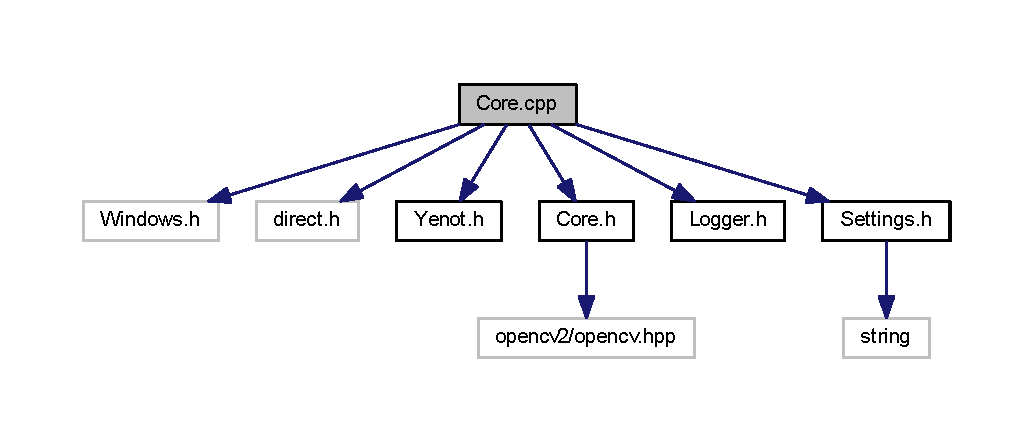
\includegraphics[width=350pt]{server_2src_2_core_8cpp__incl}
\end{center}
\end{figure}
\subsection*{Функции}
\begin{DoxyCompactItemize}
\item 
void \mbox{\hyperlink{group__corecpp_gab8ed3baad2f1d9b6b82bf74da9dd3d3a}{noise\+Removal}} (const Mat \&mat\+\_\+in, Mat \&mat\+\_\+out)
\begin{DoxyCompactList}\small\item\em Функция для обработки изображений. \end{DoxyCompactList}\item 
void \mbox{\hyperlink{group__corecpp_ga9e277d82296b5ed9eda6266d8dcc24a3}{line\+Detection}} (const Mat \&mat\+\_\+in, Mat \&mat\+\_\+out)
\begin{DoxyCompactList}\small\item\em Функция для обработки изображений. \end{DoxyCompactList}\item 
void \mbox{\hyperlink{group__corecpp_ga10a0271bceabc9c1a0d736ab93113212}{database\+Add}} (string filename)
\begin{DoxyCompactList}\small\item\em Функция для добавления файла с каскадом в файл с информацией о каскадах \end{DoxyCompactList}\item 
void \mbox{\hyperlink{group__corecpp_ga78cdbfbe907847e78cfb387df76d99f9}{clearning}} (string filename, string variable)
\begin{DoxyCompactList}\small\item\em Функция для очистки дубликатов в векторе \end{DoxyCompactList}\item 
bool \mbox{\hyperlink{group__corecpp_ga76b0b7de3d9fa0de10d66740466ebc14}{detection\+Logo}} (const Mat \&mat\+\_\+logo, string cascadefile)
\begin{DoxyCompactList}\small\item\em Функция для поиска объекта на фото \end{DoxyCompactList}\item 
void \mbox{\hyperlink{group__corecpp_gae99907f19e7f09055012f68347a57d05}{detection}} (const Mat \&mat\+\_\+logo)
\begin{DoxyCompactList}\small\item\em Модуль поиска объектов на фото \end{DoxyCompactList}\item 
void \mbox{\hyperlink{group__corecpp_ga242d25c7a9a1b7212bb890023c8131f5}{settings\+Initialization}} ()
\begin{DoxyCompactList}\small\item\em Модуль настроек. \end{DoxyCompactList}\item 
string \mbox{\hyperlink{group__corecpp_gaa85ae460901348b74381239ce0517d5f}{description}} (string value)
\begin{DoxyCompactList}\small\item\em Функция для поиска описания марки по файлу с каскадом Хаара \end{DoxyCompactList}\item 
void \mbox{\hyperlink{group__corecpp_gafe1c5d9570a4ccddf9b5105997e3ddb4}{canny}} (const Mat \&mat\+\_\+in, Mat \&mat\+\_\+out)
\begin{DoxyCompactList}\small\item\em Функция для обработки изображений. \end{DoxyCompactList}\end{DoxyCompactItemize}


\subsection{Подробное описание}
Ядро проекта. Содержит все главные и вспомогательные функции для определения марки автомобиля 

\begin{DoxyAuthor}{Автор}
Sava\+Lione 
\end{DoxyAuthor}
\begin{DoxyDate}{Дата}
12 Apr 2018 
\end{DoxyDate}

\hypertarget{tests_2src_2server_2_core_8cpp}{}\section{Файл Core.\+cpp}
\label{tests_2src_2server_2_core_8cpp}\index{Core.\+cpp@{Core.\+cpp}}
{\ttfamily \#include $<$iostream$>$}\newline
{\ttfamily \#include $<$gtest/gtest.\+h$>$}\newline
{\ttfamily \#include $<$Core.\+h$>$}\newline
{\ttfamily \#include $<$Core.\+cpp$>$}\newline
Граф включаемых заголовочных файлов для tests/src/server/\+Core.cpp\+:
\nopagebreak
\begin{figure}[H]
\begin{center}
\leavevmode
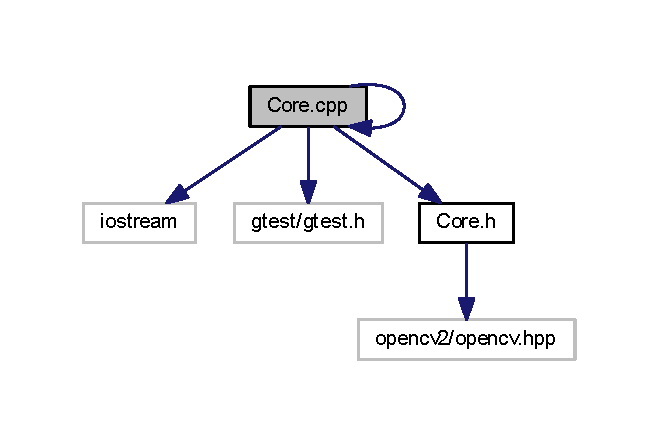
\includegraphics[width=316pt]{tests_2src_2server_2_core_8cpp__incl}
\end{center}
\end{figure}
Граф файлов, в которые включается этот файл\+:
\nopagebreak
\begin{figure}[H]
\begin{center}
\leavevmode
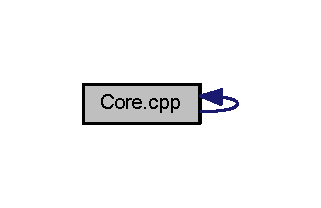
\includegraphics[width=154pt]{tests_2src_2server_2_core_8cpp__dep__incl}
\end{center}
\end{figure}
\subsection*{Функции}
\begin{DoxyCompactItemize}
\item 
\mbox{\hyperlink{group__corecpp_ga62ce880c53a3fc77fad8f0bfb8711fd9}{T\+E\+ST}} (yenot\+\_\+server\+\_\+core, inclusion)
\end{DoxyCompactItemize}


\subsection{Подробное описание}
\begin{DoxyAuthor}{Автор}
Sava\+Lione 
\end{DoxyAuthor}
\begin{DoxyDate}{Дата}
23 Jun 2018 
\end{DoxyDate}

\hypertarget{_core_8h}{}\section{Файл Core.\+h}
\label{_core_8h}\index{Core.\+h@{Core.\+h}}


Ядро проекта. Содержит все главные и вспомогательные функции для определения марки автомобиля  


{\ttfamily \#include $<$opencv2/opencv.\+hpp$>$}\newline
Граф включаемых заголовочных файлов для Core.\+h\+:
\nopagebreak
\begin{figure}[H]
\begin{center}
\leavevmode
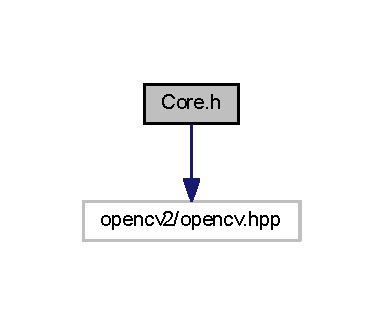
\includegraphics[width=184pt]{_core_8h__incl}
\end{center}
\end{figure}
Граф файлов, в которые включается этот файл\+:
\nopagebreak
\begin{figure}[H]
\begin{center}
\leavevmode
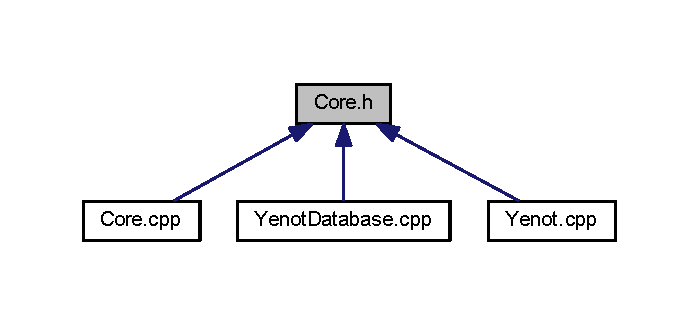
\includegraphics[width=299pt]{_core_8h__dep__incl}
\end{center}
\end{figure}
\subsection*{Функции}
\begin{DoxyCompactItemize}
\item 
void \mbox{\hyperlink{_core_8h_a438c92819ed0ad4fc2e187ed5f5a2e27}{noise\+Removal}} (const cv\+::\+Mat \&mat\+\_\+in, cv\+::\+Mat \&mat\+\_\+out)
\item 
void \mbox{\hyperlink{_core_8h_aa7c37c22318217cd913a50800eb336a3}{line\+Detection}} (const cv\+::\+Mat \&mat\+\_\+in, cv\+::\+Mat \&mat\+\_\+out)
\item 
void \mbox{\hyperlink{_core_8h_a5a4a30ca6128e13ce1ec6efaa23dd6c7}{database\+Add}} (std\+::string filename)
\item 
void \mbox{\hyperlink{_core_8h_aebd676a1476aa4d75b280db8ae09d11c}{clearning}} (std\+::string filename, std\+::string variable)
\item 
bool \mbox{\hyperlink{_core_8h_ad1ae53e92ff9edcee7a9f35d2956ae57}{detection\+Logo}} (const cv\+::\+Mat \&mat\+\_\+logo, std\+::string cascadefile)
\item 
void \mbox{\hyperlink{_core_8h_a0ef39a5ada0921b3abf8906957746b86}{detection}} (const cv\+::\+Mat \&mat\+\_\+logo)
\item 
void \mbox{\hyperlink{_core_8h_a97ee70a8770dc30d06c744b24eb2fcfc}{help}} ()
\item 
void \mbox{\hyperlink{_core_8h_a64b67e9219ba96b984256d89bc46c2f5}{blur}} (const cv\+::\+Mat \&mat\+\_\+in, cv\+::\+Mat \&mat\+\_\+out)
\item 
void \mbox{\hyperlink{_core_8h_a39eb2014e38b68bd4e6453a24e51d896}{fast\+Noise\+Removal\+Grey}} (const cv\+::\+Mat \&mat\+\_\+in, cv\+::\+Mat \&mat\+\_\+out)
\item 
void \mbox{\hyperlink{_core_8h_ab5eb0c124067d093b9001373071f4636}{fast\+Noise\+Removal}} (const cv\+::\+Mat \&mat\+\_\+in, cv\+::\+Mat \&mat\+\_\+out)
\item 
void \mbox{\hyperlink{_core_8h_aff2d42310702a0aab15af5ad62a59f2b}{canny}} (const cv\+::\+Mat \&mat\+\_\+in, cv\+::\+Mat \&mat\+\_\+out)
\item 
std\+::string \mbox{\hyperlink{_core_8h_a33e1cb874acab9d31a98a12cdd1472ce}{get\+Settings\+String}} (char $\ast$block, char $\ast$value)
\item 
std\+::string \mbox{\hyperlink{_core_8h_a3a0f1e87eb01bdd16c4a7e365aa283eb}{get\+Settings\+String}} (char $\ast$block, char $\ast$value, char $\ast$ch\+\_\+return\+\_\+default)
\item 
int \mbox{\hyperlink{_core_8h_a68b4d9ed6be7aaa93d9a6fe8fd683862}{get\+Settings}} (char $\ast$block, char $\ast$value)
\item 
int \mbox{\hyperlink{_core_8h_a0a2fe94de4037eda33c49fe332970891}{get\+Settings}} (char $\ast$block, char $\ast$value, int i\+\_\+return\+\_\+default)
\item 
void \mbox{\hyperlink{_core_8h_a463e32ccb37f9478b0e62ee0d21c5999}{set\+Settings}} (char $\ast$block, char $\ast$value, char $\ast$text)
\item 
bool \mbox{\hyperlink{_core_8h_a96c018612a57329cdb94506523f5b7ec}{check\+\_\+file}} (char $\ast$filename)
\item 
bool \mbox{\hyperlink{_core_8h_a041e0f6c7598005e2e71f7da64197d65}{check\+\_\+file}} (std\+::string filename)
\item 
void \mbox{\hyperlink{_core_8h_a8ba7f398362c96368015412b023565d0}{settings\+\_\+initialization}} ()
\item 
void \mbox{\hyperlink{_core_8h_a8f34a2030acfb5567678ab2bba25f3c1}{create\+File}} (char $\ast$file\+\_\+name)
\begin{DoxyCompactList}\small\item\em Функция для создания файла \end{DoxyCompactList}\item 
void \mbox{\hyperlink{_core_8h_a912b67f6f6b05abadd055a379dd84864}{create\+Dir}} (std\+::string namedir)
\item 
std\+::string \mbox{\hyperlink{_core_8h_aad0390ab7aa8f0cac1eee4492e919baf}{description}} (std\+::string value)
\item 
void \mbox{\hyperlink{_core_8h_aafaa59e41cfa4f5fda8c4d703394f26a}{v\+\_\+test}} ()
\begin{DoxyCompactList}\small\item\em Функция для проведения тестов. Замер скорости выполнения алгоритмов. \end{DoxyCompactList}\end{DoxyCompactItemize}


\subsection{Подробное описание}
Ядро проекта. Содержит все главные и вспомогательные функции для определения марки автомобиля 

\begin{DoxyAuthor}{Автор}
Sava\+Lione 
\end{DoxyAuthor}
\begin{DoxyDate}{Дата}
12 Apr 2018 
\end{DoxyDate}


\subsection{Функции}
\mbox{\Hypertarget{_core_8h_a64b67e9219ba96b984256d89bc46c2f5}\label{_core_8h_a64b67e9219ba96b984256d89bc46c2f5}} 
\index{Core.\+h@{Core.\+h}!blur@{blur}}
\index{blur@{blur}!Core.\+h@{Core.\+h}}
\subsubsection{\texorpdfstring{blur()}{blur()}}
{\footnotesize\ttfamily void blur (\begin{DoxyParamCaption}\item[{const cv\+::\+Mat \&}]{mat\+\_\+in,  }\item[{cv\+::\+Mat \&}]{mat\+\_\+out }\end{DoxyParamCaption})}

\mbox{\Hypertarget{_core_8h_aff2d42310702a0aab15af5ad62a59f2b}\label{_core_8h_aff2d42310702a0aab15af5ad62a59f2b}} 
\index{Core.\+h@{Core.\+h}!canny@{canny}}
\index{canny@{canny}!Core.\+h@{Core.\+h}}
\subsubsection{\texorpdfstring{canny()}{canny()}}
{\footnotesize\ttfamily void canny (\begin{DoxyParamCaption}\item[{const cv\+::\+Mat \&}]{mat\+\_\+in,  }\item[{cv\+::\+Mat \&}]{mat\+\_\+out }\end{DoxyParamCaption})}

\mbox{\Hypertarget{_core_8h_a96c018612a57329cdb94506523f5b7ec}\label{_core_8h_a96c018612a57329cdb94506523f5b7ec}} 
\index{Core.\+h@{Core.\+h}!check\+\_\+file@{check\+\_\+file}}
\index{check\+\_\+file@{check\+\_\+file}!Core.\+h@{Core.\+h}}
\subsubsection{\texorpdfstring{check\+\_\+file()}{check\_file()}\hspace{0.1cm}{\footnotesize\ttfamily [1/2]}}
{\footnotesize\ttfamily bool check\+\_\+file (\begin{DoxyParamCaption}\item[{char $\ast$}]{filename }\end{DoxyParamCaption})}



См. определение в файле Core.\+cpp строка 231

\mbox{\Hypertarget{_core_8h_a041e0f6c7598005e2e71f7da64197d65}\label{_core_8h_a041e0f6c7598005e2e71f7da64197d65}} 
\index{Core.\+h@{Core.\+h}!check\+\_\+file@{check\+\_\+file}}
\index{check\+\_\+file@{check\+\_\+file}!Core.\+h@{Core.\+h}}
\subsubsection{\texorpdfstring{check\+\_\+file()}{check\_file()}\hspace{0.1cm}{\footnotesize\ttfamily [2/2]}}
{\footnotesize\ttfamily bool check\+\_\+file (\begin{DoxyParamCaption}\item[{std\+::string}]{filename }\end{DoxyParamCaption})}

\mbox{\Hypertarget{_core_8h_aebd676a1476aa4d75b280db8ae09d11c}\label{_core_8h_aebd676a1476aa4d75b280db8ae09d11c}} 
\index{Core.\+h@{Core.\+h}!clearning@{clearning}}
\index{clearning@{clearning}!Core.\+h@{Core.\+h}}
\subsubsection{\texorpdfstring{clearning()}{clearning()}}
{\footnotesize\ttfamily void clearning (\begin{DoxyParamCaption}\item[{std\+::string}]{filename,  }\item[{std\+::string}]{variable }\end{DoxyParamCaption})}

\mbox{\Hypertarget{_core_8h_a912b67f6f6b05abadd055a379dd84864}\label{_core_8h_a912b67f6f6b05abadd055a379dd84864}} 
\index{Core.\+h@{Core.\+h}!create\+Dir@{create\+Dir}}
\index{create\+Dir@{create\+Dir}!Core.\+h@{Core.\+h}}
\subsubsection{\texorpdfstring{create\+Dir()}{createDir()}}
{\footnotesize\ttfamily void create\+Dir (\begin{DoxyParamCaption}\item[{std\+::string}]{namedir }\end{DoxyParamCaption})}

\mbox{\Hypertarget{_core_8h_a8f34a2030acfb5567678ab2bba25f3c1}\label{_core_8h_a8f34a2030acfb5567678ab2bba25f3c1}} 
\index{Core.\+h@{Core.\+h}!create\+File@{create\+File}}
\index{create\+File@{create\+File}!Core.\+h@{Core.\+h}}
\subsubsection{\texorpdfstring{create\+File()}{createFile()}}
{\footnotesize\ttfamily void create\+File (\begin{DoxyParamCaption}\item[{char $\ast$}]{file\+\_\+name }\end{DoxyParamCaption})}



Функция для создания файла 


\begin{DoxyParams}[1]{Аргументы}
\mbox{\tt in}  & {\em file\+\_\+name} & Путь и название файла \\
\hline
\end{DoxyParams}


См. определение в файле Core.\+cpp строка 288

\mbox{\Hypertarget{_core_8h_a5a4a30ca6128e13ce1ec6efaa23dd6c7}\label{_core_8h_a5a4a30ca6128e13ce1ec6efaa23dd6c7}} 
\index{Core.\+h@{Core.\+h}!database\+Add@{database\+Add}}
\index{database\+Add@{database\+Add}!Core.\+h@{Core.\+h}}
\subsubsection{\texorpdfstring{database\+Add()}{databaseAdd()}}
{\footnotesize\ttfamily void database\+Add (\begin{DoxyParamCaption}\item[{std\+::string}]{filename }\end{DoxyParamCaption})}

\mbox{\Hypertarget{_core_8h_aad0390ab7aa8f0cac1eee4492e919baf}\label{_core_8h_aad0390ab7aa8f0cac1eee4492e919baf}} 
\index{Core.\+h@{Core.\+h}!description@{description}}
\index{description@{description}!Core.\+h@{Core.\+h}}
\subsubsection{\texorpdfstring{description()}{description()}}
{\footnotesize\ttfamily std\+::string description (\begin{DoxyParamCaption}\item[{std\+::string}]{value }\end{DoxyParamCaption})}

\mbox{\Hypertarget{_core_8h_a0ef39a5ada0921b3abf8906957746b86}\label{_core_8h_a0ef39a5ada0921b3abf8906957746b86}} 
\index{Core.\+h@{Core.\+h}!detection@{detection}}
\index{detection@{detection}!Core.\+h@{Core.\+h}}
\subsubsection{\texorpdfstring{detection()}{detection()}}
{\footnotesize\ttfamily void detection (\begin{DoxyParamCaption}\item[{const cv\+::\+Mat \&}]{mat\+\_\+logo }\end{DoxyParamCaption})}

\mbox{\Hypertarget{_core_8h_ad1ae53e92ff9edcee7a9f35d2956ae57}\label{_core_8h_ad1ae53e92ff9edcee7a9f35d2956ae57}} 
\index{Core.\+h@{Core.\+h}!detection\+Logo@{detection\+Logo}}
\index{detection\+Logo@{detection\+Logo}!Core.\+h@{Core.\+h}}
\subsubsection{\texorpdfstring{detection\+Logo()}{detectionLogo()}}
{\footnotesize\ttfamily bool detection\+Logo (\begin{DoxyParamCaption}\item[{const cv\+::\+Mat \&}]{mat\+\_\+logo,  }\item[{std\+::string}]{cascadefile }\end{DoxyParamCaption})}

\mbox{\Hypertarget{_core_8h_ab5eb0c124067d093b9001373071f4636}\label{_core_8h_ab5eb0c124067d093b9001373071f4636}} 
\index{Core.\+h@{Core.\+h}!fast\+Noise\+Removal@{fast\+Noise\+Removal}}
\index{fast\+Noise\+Removal@{fast\+Noise\+Removal}!Core.\+h@{Core.\+h}}
\subsubsection{\texorpdfstring{fast\+Noise\+Removal()}{fastNoiseRemoval()}}
{\footnotesize\ttfamily void fast\+Noise\+Removal (\begin{DoxyParamCaption}\item[{const cv\+::\+Mat \&}]{mat\+\_\+in,  }\item[{cv\+::\+Mat \&}]{mat\+\_\+out }\end{DoxyParamCaption})}

\mbox{\Hypertarget{_core_8h_a39eb2014e38b68bd4e6453a24e51d896}\label{_core_8h_a39eb2014e38b68bd4e6453a24e51d896}} 
\index{Core.\+h@{Core.\+h}!fast\+Noise\+Removal\+Grey@{fast\+Noise\+Removal\+Grey}}
\index{fast\+Noise\+Removal\+Grey@{fast\+Noise\+Removal\+Grey}!Core.\+h@{Core.\+h}}
\subsubsection{\texorpdfstring{fast\+Noise\+Removal\+Grey()}{fastNoiseRemovalGrey()}}
{\footnotesize\ttfamily void fast\+Noise\+Removal\+Grey (\begin{DoxyParamCaption}\item[{const cv\+::\+Mat \&}]{mat\+\_\+in,  }\item[{cv\+::\+Mat \&}]{mat\+\_\+out }\end{DoxyParamCaption})}

\mbox{\Hypertarget{_core_8h_a68b4d9ed6be7aaa93d9a6fe8fd683862}\label{_core_8h_a68b4d9ed6be7aaa93d9a6fe8fd683862}} 
\index{Core.\+h@{Core.\+h}!get\+Settings@{get\+Settings}}
\index{get\+Settings@{get\+Settings}!Core.\+h@{Core.\+h}}
\subsubsection{\texorpdfstring{get\+Settings()}{getSettings()}\hspace{0.1cm}{\footnotesize\ttfamily [1/2]}}
{\footnotesize\ttfamily int get\+Settings (\begin{DoxyParamCaption}\item[{char $\ast$}]{block,  }\item[{char $\ast$}]{value }\end{DoxyParamCaption})}



См. определение в файле Core.\+cpp строка 219

\mbox{\Hypertarget{_core_8h_a0a2fe94de4037eda33c49fe332970891}\label{_core_8h_a0a2fe94de4037eda33c49fe332970891}} 
\index{Core.\+h@{Core.\+h}!get\+Settings@{get\+Settings}}
\index{get\+Settings@{get\+Settings}!Core.\+h@{Core.\+h}}
\subsubsection{\texorpdfstring{get\+Settings()}{getSettings()}\hspace{0.1cm}{\footnotesize\ttfamily [2/2]}}
{\footnotesize\ttfamily int get\+Settings (\begin{DoxyParamCaption}\item[{char $\ast$}]{block,  }\item[{char $\ast$}]{value,  }\item[{int}]{i\+\_\+return\+\_\+default }\end{DoxyParamCaption})}



См. определение в файле Core.\+cpp строка 223

\mbox{\Hypertarget{_core_8h_a33e1cb874acab9d31a98a12cdd1472ce}\label{_core_8h_a33e1cb874acab9d31a98a12cdd1472ce}} 
\index{Core.\+h@{Core.\+h}!get\+Settings\+String@{get\+Settings\+String}}
\index{get\+Settings\+String@{get\+Settings\+String}!Core.\+h@{Core.\+h}}
\subsubsection{\texorpdfstring{get\+Settings\+String()}{getSettingsString()}\hspace{0.1cm}{\footnotesize\ttfamily [1/2]}}
{\footnotesize\ttfamily std\+::string get\+Settings\+String (\begin{DoxyParamCaption}\item[{char $\ast$}]{block,  }\item[{char $\ast$}]{value }\end{DoxyParamCaption})}



См. определение в файле Core.\+cpp строка 207

\mbox{\Hypertarget{_core_8h_a3a0f1e87eb01bdd16c4a7e365aa283eb}\label{_core_8h_a3a0f1e87eb01bdd16c4a7e365aa283eb}} 
\index{Core.\+h@{Core.\+h}!get\+Settings\+String@{get\+Settings\+String}}
\index{get\+Settings\+String@{get\+Settings\+String}!Core.\+h@{Core.\+h}}
\subsubsection{\texorpdfstring{get\+Settings\+String()}{getSettingsString()}\hspace{0.1cm}{\footnotesize\ttfamily [2/2]}}
{\footnotesize\ttfamily std\+::string get\+Settings\+String (\begin{DoxyParamCaption}\item[{char $\ast$}]{block,  }\item[{char $\ast$}]{value,  }\item[{char $\ast$}]{ch\+\_\+return\+\_\+default }\end{DoxyParamCaption})}



См. определение в файле Core.\+cpp строка 213

\mbox{\Hypertarget{_core_8h_a97ee70a8770dc30d06c744b24eb2fcfc}\label{_core_8h_a97ee70a8770dc30d06c744b24eb2fcfc}} 
\index{Core.\+h@{Core.\+h}!help@{help}}
\index{help@{help}!Core.\+h@{Core.\+h}}
\subsubsection{\texorpdfstring{help()}{help()}}
{\footnotesize\ttfamily void help (\begin{DoxyParamCaption}{ }\end{DoxyParamCaption})}



См. определение в файле Core.\+cpp строка 136

\mbox{\Hypertarget{_core_8h_aa7c37c22318217cd913a50800eb336a3}\label{_core_8h_aa7c37c22318217cd913a50800eb336a3}} 
\index{Core.\+h@{Core.\+h}!line\+Detection@{line\+Detection}}
\index{line\+Detection@{line\+Detection}!Core.\+h@{Core.\+h}}
\subsubsection{\texorpdfstring{line\+Detection()}{lineDetection()}}
{\footnotesize\ttfamily void line\+Detection (\begin{DoxyParamCaption}\item[{const cv\+::\+Mat \&}]{mat\+\_\+in,  }\item[{cv\+::\+Mat \&}]{mat\+\_\+out }\end{DoxyParamCaption})}

\mbox{\Hypertarget{_core_8h_a438c92819ed0ad4fc2e187ed5f5a2e27}\label{_core_8h_a438c92819ed0ad4fc2e187ed5f5a2e27}} 
\index{Core.\+h@{Core.\+h}!noise\+Removal@{noise\+Removal}}
\index{noise\+Removal@{noise\+Removal}!Core.\+h@{Core.\+h}}
\subsubsection{\texorpdfstring{noise\+Removal()}{noiseRemoval()}}
{\footnotesize\ttfamily void noise\+Removal (\begin{DoxyParamCaption}\item[{const cv\+::\+Mat \&}]{mat\+\_\+in,  }\item[{cv\+::\+Mat \&}]{mat\+\_\+out }\end{DoxyParamCaption})}

\mbox{\Hypertarget{_core_8h_a463e32ccb37f9478b0e62ee0d21c5999}\label{_core_8h_a463e32ccb37f9478b0e62ee0d21c5999}} 
\index{Core.\+h@{Core.\+h}!set\+Settings@{set\+Settings}}
\index{set\+Settings@{set\+Settings}!Core.\+h@{Core.\+h}}
\subsubsection{\texorpdfstring{set\+Settings()}{setSettings()}}
{\footnotesize\ttfamily void set\+Settings (\begin{DoxyParamCaption}\item[{char $\ast$}]{block,  }\item[{char $\ast$}]{value,  }\item[{char $\ast$}]{text }\end{DoxyParamCaption})}



См. определение в файле Core.\+cpp строка 227

\mbox{\Hypertarget{_core_8h_a8ba7f398362c96368015412b023565d0}\label{_core_8h_a8ba7f398362c96368015412b023565d0}} 
\index{Core.\+h@{Core.\+h}!settings\+\_\+initialization@{settings\+\_\+initialization}}
\index{settings\+\_\+initialization@{settings\+\_\+initialization}!Core.\+h@{Core.\+h}}
\subsubsection{\texorpdfstring{settings\+\_\+initialization()}{settings\_initialization()}}
{\footnotesize\ttfamily void settings\+\_\+initialization (\begin{DoxyParamCaption}{ }\end{DoxyParamCaption})}



См. определение в файле Core.\+cpp строка 250

\mbox{\Hypertarget{_core_8h_aafaa59e41cfa4f5fda8c4d703394f26a}\label{_core_8h_aafaa59e41cfa4f5fda8c4d703394f26a}} 
\index{Core.\+h@{Core.\+h}!v\+\_\+test@{v\+\_\+test}}
\index{v\+\_\+test@{v\+\_\+test}!Core.\+h@{Core.\+h}}
\subsubsection{\texorpdfstring{v\+\_\+test()}{v\_test()}}
{\footnotesize\ttfamily void v\+\_\+test (\begin{DoxyParamCaption}{ }\end{DoxyParamCaption})}



Функция для проведения тестов. Замер скорости выполнения алгоритмов. 



См. определение в файле Core.\+cpp строка 349


\hypertarget{server_2src_2_logger_8cpp}{}\section{Файл Logger.\+cpp}
\label{server_2src_2_logger_8cpp}\index{Logger.\+cpp@{Logger.\+cpp}}


Модуль логирования. Поддерживает логирование со временем и логирование с различными уровнями.  


{\ttfamily \#include $<$Windows.\+h$>$}\newline
{\ttfamily \#include $<$fstream$>$}\newline
{\ttfamily \#include \char`\"{}Yenot.\+h\char`\"{}}\newline
{\ttfamily \#include \char`\"{}Settings.\+h\char`\"{}}\newline
Граф включаемых заголовочных файлов для server/src/\+Logger.cpp\+:
\nopagebreak
\begin{figure}[H]
\begin{center}
\leavevmode
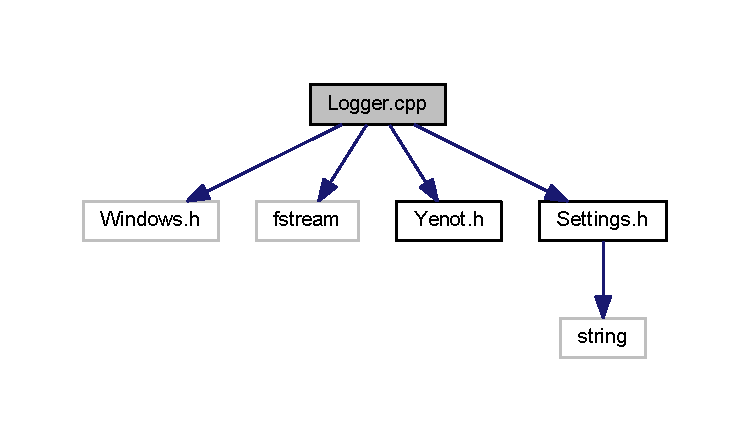
\includegraphics[width=350pt]{server_2src_2_logger_8cpp__incl}
\end{center}
\end{figure}
\subsection*{Функции}
\begin{DoxyCompactItemize}
\item 
void \mbox{\hyperlink{group__loggercpp_ga0d6abeb129096910c85ae6cba8bb59cf}{logger}} (char $\ast$level, char $\ast$text)
\begin{DoxyCompactList}\small\item\em Основная функция для логирования \end{DoxyCompactList}\end{DoxyCompactItemize}


\subsection{Подробное описание}
Модуль логирования. Поддерживает логирование со временем и логирование с различными уровнями. 

\begin{DoxyAuthor}{Автор}
Sava\+Lione 
\end{DoxyAuthor}
\begin{DoxyDate}{Дата}
1 Apr 2018 
\end{DoxyDate}

\hypertarget{tests_2src_2server_2_logger_8cpp}{}\section{Файл Logger.\+cpp}
\label{tests_2src_2server_2_logger_8cpp}\index{Logger.\+cpp@{Logger.\+cpp}}
{\ttfamily \#include $<$iostream$>$}\newline
{\ttfamily \#include $<$gtest/gtest.\+h$>$}\newline
{\ttfamily \#include $<$Logger.\+h$>$}\newline
{\ttfamily \#include $<$Logger.\+cpp$>$}\newline
Граф включаемых заголовочных файлов для tests/src/server/\+Logger.cpp\+:
\nopagebreak
\begin{figure}[H]
\begin{center}
\leavevmode
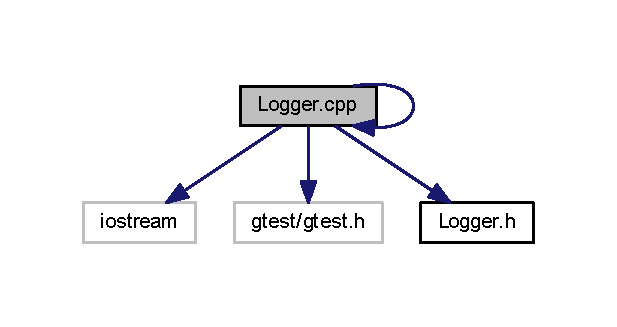
\includegraphics[width=296pt]{tests_2src_2server_2_logger_8cpp__incl}
\end{center}
\end{figure}
Граф файлов, в которые включается этот файл\+:
\nopagebreak
\begin{figure}[H]
\begin{center}
\leavevmode
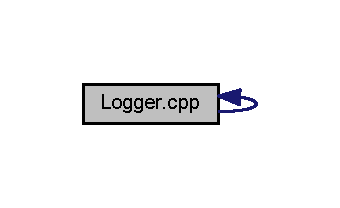
\includegraphics[width=163pt]{tests_2src_2server_2_logger_8cpp__dep__incl}
\end{center}
\end{figure}
\subsection*{Функции}
\begin{DoxyCompactItemize}
\item 
\mbox{\hyperlink{group__loggercpp_ga10abf17037baa88fa1698c6759b8c4ad}{T\+E\+ST}} (yenot\+\_\+server\+\_\+logger, inclusion)
\end{DoxyCompactItemize}


\subsection{Подробное описание}
\begin{DoxyAuthor}{Автор}
Sava\+Lione 
\end{DoxyAuthor}
\begin{DoxyDate}{Дата}
23 Jun 2018 
\end{DoxyDate}

\hypertarget{_logger_8h}{}\section{Файл Logger.\+h}
\label{_logger_8h}\index{Logger.\+h@{Logger.\+h}}


ќписание  


Граф файлов, в которые включается этот файл\+:
\nopagebreak
\begin{figure}[H]
\begin{center}
\leavevmode
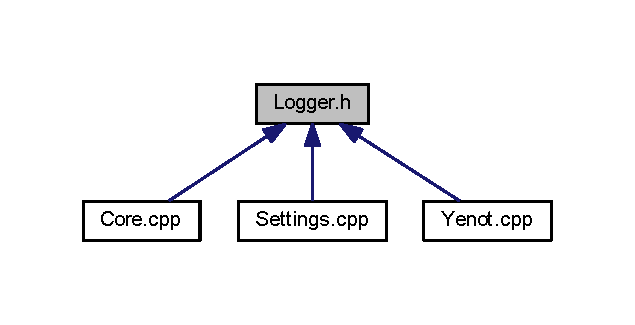
\includegraphics[width=216pt]{_logger_8h__dep__incl}
\end{center}
\end{figure}
\subsection*{Функции}
\begin{DoxyCompactItemize}
\item 
void \mbox{\hyperlink{_logger_8h_a0d6abeb129096910c85ae6cba8bb59cf}{logger}} (char $\ast$level, char $\ast$text)
\item 
void \mbox{\hyperlink{_logger_8h_a5e632a6ec68609b973a180293035b94b}{logger\+\_\+xy}} (double x, int y)
\end{DoxyCompactItemize}


\subsection{Подробное описание}
ќписание 

\begin{DoxyAuthor}{Автор}
Sava\+Lione 
\end{DoxyAuthor}


\subsection{Функции}
\mbox{\Hypertarget{_logger_8h_a0d6abeb129096910c85ae6cba8bb59cf}\label{_logger_8h_a0d6abeb129096910c85ae6cba8bb59cf}} 
\index{Logger.\+h@{Logger.\+h}!logger@{logger}}
\index{logger@{logger}!Logger.\+h@{Logger.\+h}}
\subsubsection{\texorpdfstring{logger()}{logger()}}
{\footnotesize\ttfamily void logger (\begin{DoxyParamCaption}\item[{char $\ast$}]{level,  }\item[{char $\ast$}]{text }\end{DoxyParamCaption})}



См. определение в файле Logger.\+cpp строка 11

\mbox{\Hypertarget{_logger_8h_a5e632a6ec68609b973a180293035b94b}\label{_logger_8h_a5e632a6ec68609b973a180293035b94b}} 
\index{Logger.\+h@{Logger.\+h}!logger\+\_\+xy@{logger\+\_\+xy}}
\index{logger\+\_\+xy@{logger\+\_\+xy}!Logger.\+h@{Logger.\+h}}
\subsubsection{\texorpdfstring{logger\+\_\+xy()}{logger\_xy()}}
{\footnotesize\ttfamily void logger\+\_\+xy (\begin{DoxyParamCaption}\item[{double}]{x,  }\item[{int}]{y }\end{DoxyParamCaption})}



См. определение в файле Logger.\+cpp строка 51


\hypertarget{server_2src_2_settings_8cpp}{}\section{Файл Settings.\+cpp}
\label{server_2src_2_settings_8cpp}\index{Settings.\+cpp@{Settings.\+cpp}}


Модуль работы с ini файлами  


{\ttfamily \#include $<$Windows.\+h$>$}\newline
{\ttfamily \#include $<$direct.\+h$>$}\newline
{\ttfamily \#include $<$fstream$>$}\newline
{\ttfamily \#include \char`\"{}Yenot.\+h\char`\"{}}\newline
{\ttfamily \#include \char`\"{}Logger.\+h\char`\"{}}\newline
{\ttfamily \#include \char`\"{}Settings.\+h\char`\"{}}\newline
Граф включаемых заголовочных файлов для server/src/\+Settings.cpp\+:
\nopagebreak
\begin{figure}[H]
\begin{center}
\leavevmode
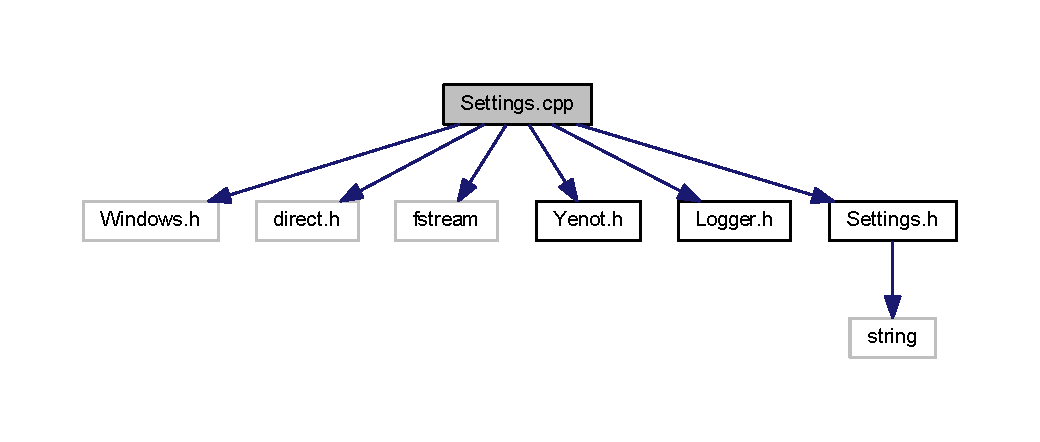
\includegraphics[width=350pt]{server_2src_2_settings_8cpp__incl}
\end{center}
\end{figure}
\subsection*{Функции}
\begin{DoxyCompactItemize}
\item 
string \mbox{\hyperlink{group__settingscpp_ga50535cebf45c8d7cbffd29274699e5f5}{get\+Settings\+String}} (char $\ast$block, char $\ast$value, char $\ast$ch\+\_\+return\+\_\+default)
\begin{DoxyCompactList}\small\item\em Получить строку из файла настроек \end{DoxyCompactList}\item 
int \mbox{\hyperlink{group__settingscpp_ga0a2fe94de4037eda33c49fe332970891}{get\+Settings}} (char $\ast$block, char $\ast$value, int i\+\_\+return\+\_\+default)
\begin{DoxyCompactList}\small\item\em Получить число из файла настроек \end{DoxyCompactList}\item 
void \mbox{\hyperlink{group__settingscpp_ga463e32ccb37f9478b0e62ee0d21c5999}{set\+Settings}} (char $\ast$block, char $\ast$value, char $\ast$text)
\begin{DoxyCompactList}\small\item\em Сохранить переменную в файл настроек \end{DoxyCompactList}\item 
bool \mbox{\hyperlink{group__settingscpp_ga2dd1bc039652a0480c444957d416b6a6}{check\+File}} (char $\ast$filename)
\begin{DoxyCompactList}\small\item\em Проверка файла \end{DoxyCompactList}\item 
bool \mbox{\hyperlink{group__settingscpp_ga64f8c9899c815dc180b2b564c0d05762}{check\+File}} (string filename)
\begin{DoxyCompactList}\small\item\em Проверка файла \end{DoxyCompactList}\item 
void \mbox{\hyperlink{group__settingscpp_ga5ac0cd45ecb6e65e3ace40687d6ee8bc}{create\+Dir}} (string namedir)
\begin{DoxyCompactList}\small\item\em Функция для создания директории \end{DoxyCompactList}\item 
void \mbox{\hyperlink{group__settingscpp_ga8f34a2030acfb5567678ab2bba25f3c1}{create\+File}} (char $\ast$file\+\_\+name)
\begin{DoxyCompactList}\small\item\em Функция для создания файла \end{DoxyCompactList}\end{DoxyCompactItemize}


\subsection{Подробное описание}
Модуль работы с ini файлами 

\begin{DoxyAuthor}{Автор}
Sava\+Lione 
\end{DoxyAuthor}
\begin{DoxyDate}{Дата}
20 Apr 2018 
\end{DoxyDate}

\hypertarget{tests_2src_2server_2_settings_8cpp}{}\section{Файл Settings.\+cpp}
\label{tests_2src_2server_2_settings_8cpp}\index{Settings.\+cpp@{Settings.\+cpp}}
{\ttfamily \#include $<$iostream$>$}\newline
{\ttfamily \#include $<$gtest/gtest.\+h$>$}\newline
{\ttfamily \#include $<$Settings.\+h$>$}\newline
{\ttfamily \#include $<$Settings.\+cpp$>$}\newline
Граф включаемых заголовочных файлов для tests/src/server/\+Settings.cpp\+:
\nopagebreak
\begin{figure}[H]
\begin{center}
\leavevmode
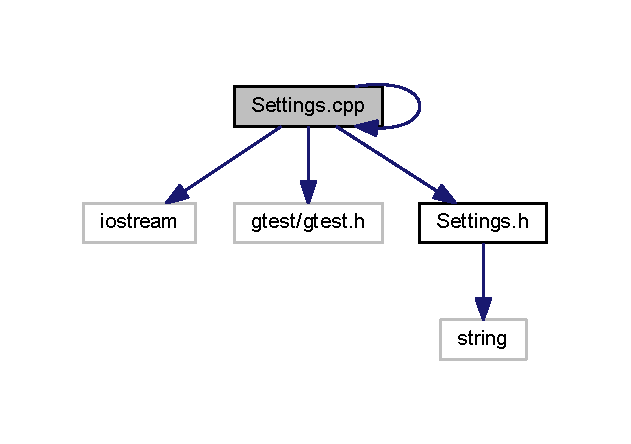
\includegraphics[width=303pt]{tests_2src_2server_2_settings_8cpp__incl}
\end{center}
\end{figure}
Граф файлов, в которые включается этот файл\+:
\nopagebreak
\begin{figure}[H]
\begin{center}
\leavevmode
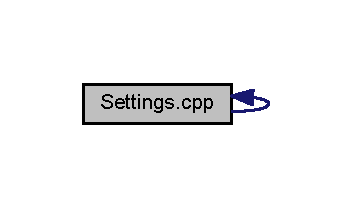
\includegraphics[width=169pt]{tests_2src_2server_2_settings_8cpp__dep__incl}
\end{center}
\end{figure}
\subsection*{Функции}
\begin{DoxyCompactItemize}
\item 
\mbox{\hyperlink{group__settingscpp_ga1313defba35762697f41324fbd47171d}{T\+E\+ST}} (yenot\+\_\+server\+\_\+settings, inclusion)
\end{DoxyCompactItemize}


\subsection{Подробное описание}
\begin{DoxyAuthor}{Автор}
Sava\+Lione 
\end{DoxyAuthor}
\begin{DoxyDate}{Дата}
23 Jun 2018 
\end{DoxyDate}

\hypertarget{_settings_8h}{}\section{Файл Settings.\+h}
\label{_settings_8h}\index{Settings.\+h@{Settings.\+h}}


Заголовочный файл модуля работы с ini файлами  


{\ttfamily \#include $<$string$>$}\newline
Граф включаемых заголовочных файлов для Settings.\+h\+:
\nopagebreak
\begin{figure}[H]
\begin{center}
\leavevmode
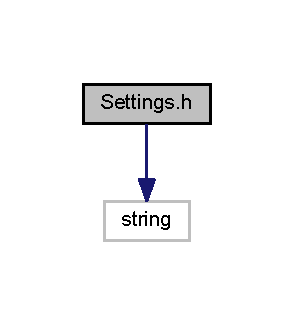
\includegraphics[width=141pt]{_settings_8h__incl}
\end{center}
\end{figure}
Граф файлов, в которые включается этот файл\+:
\nopagebreak
\begin{figure}[H]
\begin{center}
\leavevmode
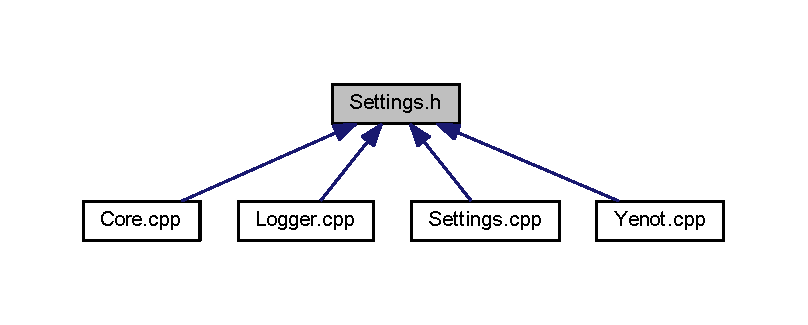
\includegraphics[width=350pt]{_settings_8h__dep__incl}
\end{center}
\end{figure}
\subsection*{Функции}
\begin{DoxyCompactItemize}
\item 
std\+::string \mbox{\hyperlink{group__settingsh_ga3a0f1e87eb01bdd16c4a7e365aa283eb}{get\+Settings\+String}} (char $\ast$block, char $\ast$value, char $\ast$ch\+\_\+return\+\_\+default)
\item 
int \mbox{\hyperlink{group__settingsh_ga68b4d9ed6be7aaa93d9a6fe8fd683862}{get\+Settings}} (char $\ast$block, char $\ast$value)
\item 
int \mbox{\hyperlink{group__settingsh_ga0a2fe94de4037eda33c49fe332970891}{get\+Settings}} (char $\ast$block, char $\ast$value, int i\+\_\+return\+\_\+default)
\item 
void \mbox{\hyperlink{group__settingsh_ga463e32ccb37f9478b0e62ee0d21c5999}{set\+Settings}} (char $\ast$block, char $\ast$value, char $\ast$text)
\item 
bool \mbox{\hyperlink{group__settingsh_ga2dd1bc039652a0480c444957d416b6a6}{check\+File}} (char $\ast$filename)
\item 
bool \mbox{\hyperlink{group__settingsh_ga147bed619c6314e960320c1bcb40ed91}{check\+File}} (std\+::string filename)
\item 
void \mbox{\hyperlink{group__settingsh_ga8f34a2030acfb5567678ab2bba25f3c1}{create\+File}} (char $\ast$file\+\_\+name)
\begin{DoxyCompactList}\small\item\em Функция для создания файла \end{DoxyCompactList}\item 
void \mbox{\hyperlink{group__settingsh_ga912b67f6f6b05abadd055a379dd84864}{create\+Dir}} (std\+::string namedir)
\end{DoxyCompactItemize}


\subsection{Подробное описание}
Заголовочный файл модуля работы с ini файлами 

\begin{DoxyAuthor}{Автор}
Sava\+Lione 
\end{DoxyAuthor}
\begin{DoxyDate}{Дата}
20 Apr 2018 
\end{DoxyDate}

\hypertarget{_test_8cpp}{}\section{Файл Test.\+cpp}
\label{_test_8cpp}\index{Test.\+cpp@{Test.\+cpp}}


Модуль тестирования  


{\ttfamily \#include $<$iostream$>$}\newline
{\ttfamily \#include $<$gtest/gtest.\+h$>$}\newline
{\ttfamily \#include $<$Core.\+h$>$}\newline
Граф включаемых заголовочных файлов для Test.\+cpp\+:
\nopagebreak
\begin{figure}[H]
\begin{center}
\leavevmode
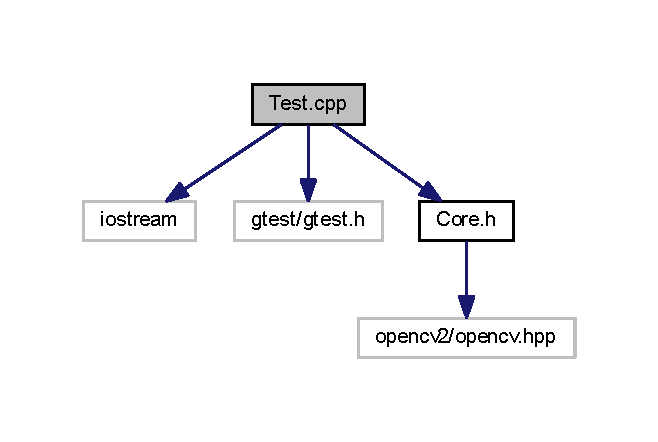
\includegraphics[width=316pt]{_test_8cpp__incl}
\end{center}
\end{figure}
\subsection*{Функции}
\begin{DoxyCompactItemize}
\item 
\mbox{\hyperlink{group__testcpp_ga0c6e823009aa80ab758989270ff8eec2}{T\+E\+ST}} (yenot\+\_\+test, correct\+\_\+connection\+\_\+testing\+\_\+module)
\end{DoxyCompactItemize}


\subsection{Подробное описание}
Модуль тестирования 

\begin{DoxyAuthor}{Автор}
Sava\+Lione 
\end{DoxyAuthor}
\begin{DoxyDate}{Дата}
23 Jun 2018 
\end{DoxyDate}

\hypertarget{_yenot_8cpp}{}\section{Файл Yenot.\+cpp}
\label{_yenot_8cpp}\index{Yenot.\+cpp@{Yenot.\+cpp}}


Описание  


{\ttfamily \#include \char`\"{}..\textbackslash{}core\textbackslash{}\+Yenot.\+h\char`\"{}}\newline
{\ttfamily \#include \char`\"{}..\textbackslash{}core\textbackslash{}\+Core.\+h\char`\"{}}\newline
{\ttfamily \#include \char`\"{}..\textbackslash{}io\textbackslash{}\+Logger.\+h\char`\"{}}\newline
Граф включаемых заголовочных файлов для Yenot.\+cpp\+:
\nopagebreak
\begin{figure}[H]
\begin{center}
\leavevmode
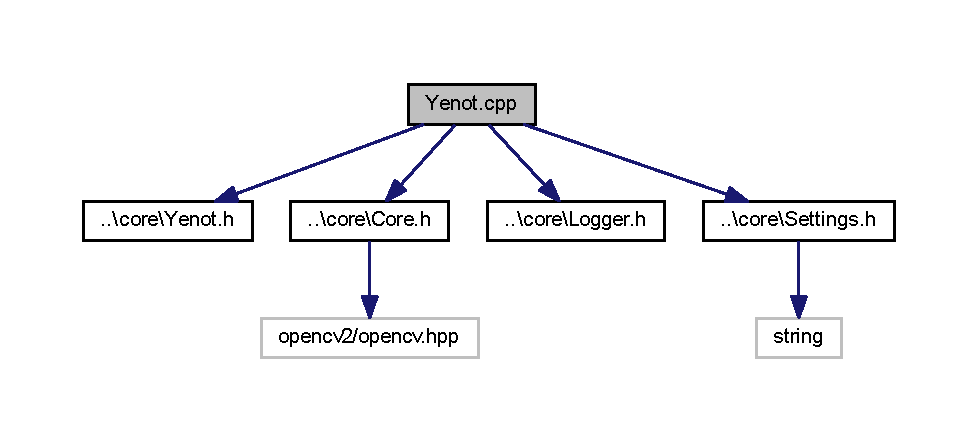
\includegraphics[width=348pt]{_yenot_8cpp__incl}
\end{center}
\end{figure}
\subsection*{Функции}
\begin{DoxyCompactItemize}
\item 
int \mbox{\hyperlink{_yenot_8cpp_a0ddf1224851353fc92bfbff6f499fa97}{main}} (int argc, char $\ast$argv\mbox{[}$\,$\mbox{]})
\end{DoxyCompactItemize}


\subsection{Подробное описание}
Описание 

\begin{DoxyAuthor}{Автор}
Sava\+Lione 
\end{DoxyAuthor}
\begin{DoxyDate}{Дата}
28 Mar 2018 
\end{DoxyDate}


\subsection{Функции}
\mbox{\Hypertarget{_yenot_8cpp_a0ddf1224851353fc92bfbff6f499fa97}\label{_yenot_8cpp_a0ddf1224851353fc92bfbff6f499fa97}} 
\index{Yenot.\+cpp@{Yenot.\+cpp}!main@{main}}
\index{main@{main}!Yenot.\+cpp@{Yenot.\+cpp}}
\subsubsection{\texorpdfstring{main()}{main()}}
{\footnotesize\ttfamily int main (\begin{DoxyParamCaption}\item[{int}]{argc,  }\item[{char $\ast$}]{argv\mbox{[}$\,$\mbox{]} }\end{DoxyParamCaption})}



См. определение в файле Yenot.\+cpp строка 15


\hypertarget{_yenot_8h}{}\section{Файл Yenot.\+h}
\label{_yenot_8h}\index{Yenot.\+h@{Yenot.\+h}}


Заголовочный файл с пространством имён, которое хранит в себе константы.  


Граф файлов, в которые включается этот файл\+:
\nopagebreak
\begin{figure}[H]
\begin{center}
\leavevmode
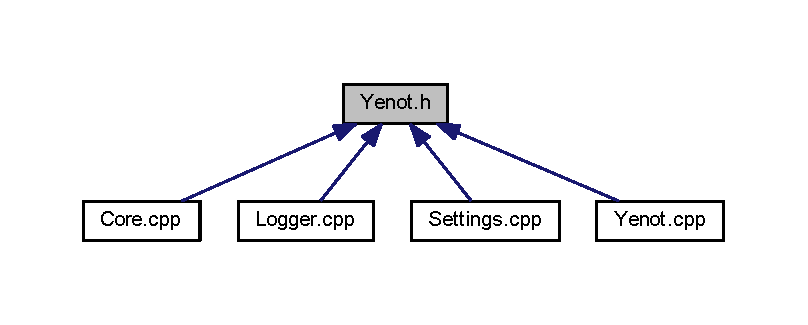
\includegraphics[width=350pt]{_yenot_8h__dep__incl}
\end{center}
\end{figure}
\subsection*{Пространства имен}
\begin{DoxyCompactItemize}
\item 
 \mbox{\hyperlink{namespaceyenot}{yenot}}
\begin{DoxyCompactList}\small\item\em Пространство имён с константами \end{DoxyCompactList}\end{DoxyCompactItemize}
\subsection*{Переменные}
\begin{DoxyCompactItemize}
\item 
const char \mbox{\hyperlink{namespaceyenot_a376e7adfbabcae01c8305ed17d47d576}{yenot\+::\+F\+I\+L\+E\+\_\+\+N\+A\+M\+E\+\_\+\+C\+O\+N\+F\+IG}} \mbox{[}$\,$\mbox{]} = \char`\"{}./config.\+ini\char`\"{}
\begin{DoxyCompactList}\small\item\em Файл с настройками \end{DoxyCompactList}\item 
const char \mbox{\hyperlink{namespaceyenot_a6fdda6751433c679b7976669aff150b8}{yenot\+::\+F\+I\+L\+E\+\_\+\+N\+A\+M\+E\+\_\+\+L\+O\+G\+G\+ER}} \mbox{[}$\,$\mbox{]} = \char`\"{}Yenot.\+log\char`\"{}
\begin{DoxyCompactList}\small\item\em Файл с логами \end{DoxyCompactList}\item 
const char \mbox{\hyperlink{namespaceyenot_ae254e34a07790b92c8085e559be10f38}{yenot\+::\+F\+I\+L\+E\+\_\+\+N\+A\+M\+E\+\_\+\+D\+A\+T\+A\+B\+A\+SE}} \mbox{[}$\,$\mbox{]} = \char`\"{}database.\+xml\char`\"{}
\begin{DoxyCompactList}\small\item\em Файл, в котором хранятся \end{DoxyCompactList}\item 
const char \mbox{\hyperlink{namespaceyenot_af2253e95acd84452c01f492019f814f0}{yenot\+::\+N\+A\+M\+E\+\_\+\+D\+A\+T\+A\+B\+A\+SE}} \mbox{[}$\,$\mbox{]} = \char`\"{}database\char`\"{}
\item 
const char \mbox{\hyperlink{namespaceyenot_aa5230dc84adb2ca08b014531f83cd3c9}{yenot\+::\+E\+X\+T\+E\+N\+S\+I\+O\+N\+S\+\_\+\+D\+A\+T\+A\+B\+A\+S\+E\+\_\+\+M\+E\+M\+B\+ER}} \mbox{[}$\,$\mbox{]} = \char`\"{}.xml\char`\"{}
\item 
const char \mbox{\hyperlink{namespaceyenot_abf6ea7d0c605b7432754b26575046d32}{yenot\+::\+E\+X\+T\+E\+N\+S\+I\+O\+N\+S\+\_\+\+D\+A\+T\+A\+B\+A\+S\+E\+\_\+\+M\+E\+M\+B\+E\+R\+\_\+photo}} \mbox{[}$\,$\mbox{]} = \char`\"{}.png\char`\"{}
\item 
const int \mbox{\hyperlink{namespaceyenot_a08846c7b8addedd4db68b5cf3721bda1}{yenot\+::\+B\+U\+F\+F\+E\+R\+\_\+\+S\+I\+ZE}} = 128
\begin{DoxyCompactList}\small\item\em Стандартный размер буфера \end{DoxyCompactList}\item 
const char \mbox{\hyperlink{namespaceyenot_a2172a9f506029215b790a51a4023e1ac}{yenot\+::\+B\+L\+O\+C\+K\+\_\+\+C\+O\+RE}} \mbox{[}$\,$\mbox{]} = \char`\"{}Core\char`\"{}
\item 
const char \mbox{\hyperlink{namespaceyenot_a254a74c9007fa3d541605ff059a74add}{yenot\+::\+S\+E\+T\+T\+I\+N\+G\+S\+\_\+\+F\+A\+S\+T\+M\+O\+DE}} \mbox{[}$\,$\mbox{]} = \char`\"{}f\+Mode\char`\"{}
\item 
const char \mbox{\hyperlink{namespaceyenot_a7afad42fc42152730906aa57ef688c9a}{yenot\+::\+S\+E\+T\+T\+I\+N\+G\+S\+\_\+\+F\+A\+S\+T\+M\+O\+D\+E\+\_\+\+V\+A\+L\+UE}} \mbox{[}$\,$\mbox{]} = \char`\"{}0\char`\"{}
\item 
const int \mbox{\hyperlink{namespaceyenot_aef79e343f25022f42e779be319348eec}{yenot\+::\+S\+E\+T\+T\+I\+N\+G\+S\+\_\+\+F\+A\+S\+T\+M\+O\+D\+E\+\_\+\+V\+A\+L\+U\+E\+\_\+\+I\+NT}} = 0
\item 
const char \mbox{\hyperlink{namespaceyenot_a01aebb6f9dc4632eabd3ef606f5c75fb}{yenot\+::\+S\+E\+T\+T\+I\+N\+G\+S\+\_\+\+N\+O\+I\+S\+E\+\_\+\+R\+E\+D\+U\+C\+T\+I\+ON}} \mbox{[}$\,$\mbox{]} = \char`\"{}n\+Reduction\char`\"{}
\item 
const char \mbox{\hyperlink{namespaceyenot_a557e3ad9f3290543eed07f92644f1e33}{yenot\+::\+S\+E\+T\+T\+I\+N\+G\+S\+\_\+\+N\+O\+I\+S\+E\+\_\+\+R\+E\+D\+U\+C\+T\+I\+O\+N\+\_\+\+V\+A\+L\+UE}} \mbox{[}$\,$\mbox{]} = \char`\"{}1\char`\"{}
\item 
const int \mbox{\hyperlink{namespaceyenot_aaaef89f90413ee7a52a64d043e068136}{yenot\+::\+S\+E\+T\+T\+I\+N\+G\+S\+\_\+\+N\+O\+I\+S\+E\+\_\+\+R\+E\+D\+U\+C\+T\+I\+O\+N\+\_\+\+V\+A\+L\+U\+E\+\_\+\+I\+NT}} = 1
\item 
const char \mbox{\hyperlink{namespaceyenot_a6d4d3d03406bad7102e67e0f0d81edc2}{yenot\+::\+S\+E\+T\+T\+I\+N\+G\+S\+\_\+\+L\+I\+N\+E\+\_\+\+D\+E\+T\+E\+C\+T\+I\+ON}} \mbox{[}$\,$\mbox{]} = \char`\"{}l\+Detection\char`\"{}
\item 
const char \mbox{\hyperlink{namespaceyenot_ae8e9b52935a937554723960a8933df49}{yenot\+::\+S\+E\+T\+T\+I\+N\+G\+S\+\_\+\+L\+I\+N\+E\+\_\+\+D\+E\+T\+E\+C\+T\+I\+O\+N\+\_\+\+V\+A\+L\+UE}} \mbox{[}$\,$\mbox{]} = \char`\"{}1\char`\"{}
\item 
const int \mbox{\hyperlink{namespaceyenot_a07cb3f48df07dea977024678d96871f8}{yenot\+::\+S\+E\+T\+T\+I\+N\+G\+S\+\_\+\+L\+I\+N\+E\+\_\+\+D\+E\+T\+E\+C\+T\+I\+O\+N\+\_\+\+V\+A\+L\+U\+E\+\_\+\+I\+NT}} = 1
\item 
const char \mbox{\hyperlink{namespaceyenot_a6a7294929420d7790b72f733c98bcf56}{yenot\+::\+S\+E\+T\+T\+I\+N\+G\+S\+\_\+\+D\+E\+T\+E\+C\+T\+I\+ON}} \mbox{[}$\,$\mbox{]} = \char`\"{}detection\char`\"{}
\item 
const char \mbox{\hyperlink{namespaceyenot_a7d631c2848347b1df2d133225075ced0}{yenot\+::\+S\+E\+T\+T\+I\+N\+G\+S\+\_\+\+D\+E\+T\+E\+C\+T\+I\+O\+N\+\_\+\+V\+A\+L\+UE}} \mbox{[}$\,$\mbox{]} = \char`\"{}1\char`\"{}
\item 
const int \mbox{\hyperlink{namespaceyenot_a3043cfcdd8cc01993a692d71244049f6}{yenot\+::\+S\+E\+T\+T\+I\+N\+G\+S\+\_\+\+D\+E\+T\+E\+C\+T\+I\+O\+N\+\_\+\+V\+A\+L\+U\+E\+\_\+\+I\+NT}} = 1
\item 
const char \mbox{\hyperlink{namespaceyenot_a68308c1bd5623fffdc0992da59a687b3}{yenot\+::\+S\+E\+T\+T\+I\+N\+G\+S\+\_\+\+S\+A\+V\+E\+\_\+\+P\+R\+O\+C\+E\+S\+S\+E\+D\+\_\+\+I\+M\+A\+GE}} \mbox{[}$\,$\mbox{]} = \char`\"{}s\+Image\char`\"{}
\item 
const char \mbox{\hyperlink{namespaceyenot_a2e3ae4b394042b1c4cbc4ae56a4af012}{yenot\+::\+S\+E\+T\+T\+I\+N\+G\+S\+\_\+\+S\+A\+V\+E\+\_\+\+P\+R\+O\+C\+E\+S\+S\+E\+D\+\_\+\+I\+M\+A\+G\+E\+\_\+\+V\+A\+L\+UE}} \mbox{[}$\,$\mbox{]} = \char`\"{}0\char`\"{}
\item 
const int \mbox{\hyperlink{namespaceyenot_a58502c9277df0f0d680ddc344e5cea3e}{yenot\+::\+S\+E\+T\+T\+I\+N\+G\+S\+\_\+\+S\+A\+V\+E\+\_\+\+P\+R\+O\+C\+E\+S\+S\+E\+D\+\_\+\+I\+M\+A\+G\+E\+\_\+\+V\+A\+L\+U\+E\+\_\+\+I\+NT}} = 0
\item 
const char \mbox{\hyperlink{namespaceyenot_a6703c9900f97a42185c36c74c4147be3}{yenot\+::\+S\+E\+T\+T\+I\+N\+G\+S\+\_\+\+S\+A\+V\+E\+\_\+\+P\+R\+O\+C\+E\+S\+S\+E\+D\+\_\+\+I\+M\+A\+G\+E\+\_\+\+N\+A\+ME}} \mbox{[}$\,$\mbox{]} = \char`\"{}test.\+png\char`\"{}
\item 
const char \mbox{\hyperlink{namespaceyenot_a353e320b6fbef3dc210fd42ad10ff83c}{yenot\+::\+S\+E\+T\+T\+I\+N\+G\+S\+\_\+\+L\+OG}} \mbox{[}$\,$\mbox{]} = \char`\"{}log\char`\"{}
\item 
const char \mbox{\hyperlink{namespaceyenot_ab2eea8a981ab7baa7755cc64508671a0}{yenot\+::\+S\+E\+T\+T\+I\+N\+G\+S\+\_\+\+L\+O\+G\+\_\+\+V\+A\+L\+UE}} \mbox{[}$\,$\mbox{]} = \char`\"{}1\char`\"{}
\item 
const int \mbox{\hyperlink{namespaceyenot_ab756a3a6fb449bd27e6674cdf402b4d1}{yenot\+::\+S\+E\+T\+T\+I\+N\+G\+S\+\_\+\+L\+O\+G\+\_\+\+V\+A\+L\+U\+E\+\_\+\+I\+NT}} = 1
\item 
const char \mbox{\hyperlink{namespaceyenot_a420dc7e6e8223c7cd5ec7127995d46a0}{yenot\+::\+S\+E\+T\+T\+I\+N\+G\+S\+\_\+\+L\+O\+G\+\_\+\+T\+I\+ME}} \mbox{[}$\,$\mbox{]} = \char`\"{}l\+Time\char`\"{}
\item 
const char \mbox{\hyperlink{namespaceyenot_ae00932245c3089d385ef8ee3463df8ca}{yenot\+::\+S\+E\+T\+T\+I\+N\+G\+S\+\_\+\+L\+O\+G\+\_\+\+T\+I\+M\+E\+\_\+\+V\+A\+L\+UE}} \mbox{[}$\,$\mbox{]} = \char`\"{}1\char`\"{}
\item 
const int \mbox{\hyperlink{namespaceyenot_abc8b052e7f097163709fa71c4da4478d}{yenot\+::\+S\+E\+T\+T\+I\+N\+G\+S\+\_\+\+L\+O\+G\+\_\+\+T\+I\+M\+E\+\_\+\+V\+A\+L\+U\+E\+\_\+\+I\+NT}} = 1
\item 
const char \mbox{\hyperlink{namespaceyenot_a347fa05f62ae28e55301db755cf26210}{yenot\+::\+S\+E\+T\+T\+I\+N\+G\+S\+\_\+\+T\+E\+M\+P\+L\+A\+T\+E\+\_\+\+S\+I\+ZE}} \mbox{[}$\,$\mbox{]} = \char`\"{}templatesize\char`\"{}
\item 
const char \mbox{\hyperlink{namespaceyenot_acfc97705229a010013bb0433327bf707}{yenot\+::\+T\+E\+M\+P\+L\+A\+T\+E\+\_\+\+S\+I\+Z\+E\+\_\+\+S\+TR}} \mbox{[}$\,$\mbox{]} = \char`\"{}20\char`\"{}
\item 
const int \mbox{\hyperlink{namespaceyenot_a6c04317b4747d569efcf92266bb1051b}{yenot\+::\+T\+E\+M\+P\+L\+A\+T\+E\+\_\+\+S\+I\+ZE}} = 20
\item 
const char \mbox{\hyperlink{namespaceyenot_a6a132f52235e5b9454c850b4f5343ce3}{yenot\+::\+S\+E\+T\+T\+I\+N\+G\+S\+\_\+\+S\+I\+Z\+E\+\_\+\+P\+H\+O\+TO}} \mbox{[}$\,$\mbox{]} = \char`\"{}size\+Photo\char`\"{}
\item 
const char \mbox{\hyperlink{namespaceyenot_a172f1253ba2c664d26caffab97a6253d}{yenot\+::\+S\+I\+Z\+E\+\_\+\+P\+H\+O\+T\+O\+\_\+\+S\+TR}} \mbox{[}$\,$\mbox{]} = \char`\"{}512\char`\"{}
\item 
const int \mbox{\hyperlink{namespaceyenot_a501462c649059c5efe3019823a607670}{yenot\+::\+S\+I\+Z\+E\+\_\+\+P\+H\+O\+TO}} = 512
\item 
const int \mbox{\hyperlink{namespaceyenot_ad85720cad8409ab5ef5cc47afc84645c}{yenot\+::\+D\+I\+A\+M\+E\+T\+E\+R\+\_\+\+E\+A\+C\+H\+\_\+\+P\+I\+X\+EL}} = 9
\item 
const int \mbox{\hyperlink{namespaceyenot_affd7404833d15c98fbd85249f43f98da}{yenot\+::\+S\+I\+G\+M\+A\+\_\+\+C\+O\+L\+OR}} = 75
\item 
const int \mbox{\hyperlink{namespaceyenot_ad45191f613b95ca3398e6eab5e202406}{yenot\+::\+S\+I\+G\+M\+A\+\_\+\+S\+P\+A\+CE}} = 75
\item 
const int \mbox{\hyperlink{namespaceyenot_aa753d0e3e99fb4b37b3930996bdfe563}{yenot\+::\+K\+E\+R\+N\+E\+L\+\_\+X}} = 5
\item 
const int \mbox{\hyperlink{namespaceyenot_a33a5af73a30e2b5684ee02cc4bf4c374}{yenot\+::\+K\+E\+R\+N\+E\+L\+\_\+Y}} = 5
\item 
const char \mbox{\hyperlink{namespaceyenot_a73be0cdcde2af378cd4043f56d4776e2}{yenot\+::\+B\+L\+O\+C\+K\+\_\+\+L\+O\+G\+G\+ER}} \mbox{[}$\,$\mbox{]} = \char`\"{}Logger\char`\"{}
\item 
const char \mbox{\hyperlink{namespaceyenot_a1133c576c0c3eebe5aa6c43529a56f21}{yenot\+::\+L\+O\+G\+G\+E\+R\+\_\+\+L\+E\+V\+E\+L\+\_\+\+W\+A\+R\+N\+I\+NG}} \mbox{[}$\,$\mbox{]} = \char`\"{}W\+A\+RN\char`\"{}
\begin{DoxyCompactList}\small\item\em Уровень предупреждения \end{DoxyCompactList}\item 
const char \mbox{\hyperlink{namespaceyenot_a08c0d88b074bcba3b7d79d019211a1ac}{yenot\+::\+L\+O\+G\+G\+E\+R\+\_\+\+L\+E\+V\+E\+L\+\_\+\+E\+R\+R\+OR}} \mbox{[}$\,$\mbox{]} = \char`\"{}E\+R\+R\+OR\char`\"{}
\begin{DoxyCompactList}\small\item\em Уровень ошибки \end{DoxyCompactList}\item 
const char \mbox{\hyperlink{namespaceyenot_a75d435531623705520a8bd478ae6e3ed}{yenot\+::\+L\+O\+G\+G\+E\+R\+\_\+\+L\+E\+V\+E\+L\+\_\+\+M\+E\+S\+S\+A\+GE}} \mbox{[}$\,$\mbox{]} = \char`\"{}M\+SG\char`\"{}
\begin{DoxyCompactList}\small\item\em Уровень сообщение \end{DoxyCompactList}\item 
const char \mbox{\hyperlink{namespaceyenot_ae3c6bd195ef1c9bdcbd48e5b44e17aaf}{yenot\+::\+L\+O\+G\+G\+E\+R\+\_\+\+M\+E\+S\+S\+A\+G\+E\+\_\+\+N\+O\+I\+S\+E\+\_\+\+R\+E\+M\+O\+V\+AL}} \mbox{[}$\,$\mbox{]} = \char`\"{}Noise filter is disabled.\char`\"{}
\begin{DoxyCompactList}\small\item\em Сообщение в лог о том, что фильтр шума отключен \end{DoxyCompactList}\item 
const char \mbox{\hyperlink{namespaceyenot_a3cc24a045a30435ab78be6014ff26a16}{yenot\+::\+L\+O\+G\+G\+E\+R\+\_\+\+M\+E\+S\+S\+A\+G\+E\+\_\+\+L\+I\+N\+E\+\_\+\+D\+E\+T\+E\+C\+T\+I\+ON}} \mbox{[}$\,$\mbox{]} = \char`\"{}Line \mbox{\hyperlink{group__coreh_ga0ef39a5ada0921b3abf8906957746b86}{detection}} is disabled.\char`\"{}
\begin{DoxyCompactList}\small\item\em Сообщение в лог о том, что детектор границ отключен \end{DoxyCompactList}\item 
const char \mbox{\hyperlink{namespaceyenot_a23d265aa1784a96ebe7ce76bedd308a6}{yenot\+::\+L\+O\+G\+G\+E\+R\+\_\+\+M\+E\+S\+S\+A\+G\+E\+\_\+\+F\+A\+S\+T\+\_\+\+M\+O\+DE}} \mbox{[}$\,$\mbox{]} = \char`\"{}Fast mode enabled.\char`\"{}
\begin{DoxyCompactList}\small\item\em Сообщение в лог о том, что быстрый режим включен \end{DoxyCompactList}\item 
const char \mbox{\hyperlink{namespaceyenot_ace626bb1b7477b39cf2864aa0d0924e9}{yenot\+::\+L\+O\+G\+G\+E\+R\+\_\+\+M\+E\+S\+S\+A\+G\+E\+\_\+\+C\+R\+E\+A\+T\+E\+\_\+\+D\+IR}} \mbox{[}$\,$\mbox{]} = \char`\"{}Folder created.\char`\"{}
\begin{DoxyCompactList}\small\item\em Сообщение в лог о том, что папка создана \end{DoxyCompactList}\item 
const char \mbox{\hyperlink{namespaceyenot_ae73ee066dad5c6455cb406ab3aa0473f}{yenot\+::\+L\+O\+G\+G\+E\+R\+\_\+\+M\+E\+S\+S\+A\+G\+E\+\_\+\+C\+R\+E\+A\+T\+E\+\_\+\+D\+I\+R\+\_\+\+N\+OT}} \mbox{[}$\,$\mbox{]} = \char`\"{}Folder creation failed.\char`\"{}
\begin{DoxyCompactList}\small\item\em Сообщение в лог о том, что не удалось создать папку \end{DoxyCompactList}\item 
const int \mbox{\hyperlink{namespaceyenot_a8206ed93e65c9e89395c2823a5f18786}{yenot\+::\+E\+R\+R\+O\+R\+\_\+\+I\+N\+IT}} = -\/100
\begin{DoxyCompactList}\small\item\em Ошибка инициализации \end{DoxyCompactList}\item 
const int \mbox{\hyperlink{namespaceyenot_a3c1c146cfa3fc68ce0e1950b93270849}{yenot\+::\+E\+R\+R\+O\+R\+\_\+\+I\+M\+A\+GE}} = -\/200
\begin{DoxyCompactList}\small\item\em Ошибка связанная с входным изображением. Возможно не достаточно аргументов \end{DoxyCompactList}\item 
const int \mbox{\hyperlink{namespaceyenot_a9b11e5890ebee4b3ace81f058483b7af}{yenot\+::\+E\+R\+R\+O\+R\+\_\+\+C\+L\+E\+A\+R\+N\+I\+NG}} = -\/300
\begin{DoxyCompactList}\small\item\em Ошибка связанная с очисткой дубликатов \end{DoxyCompactList}\item 
const int \mbox{\hyperlink{namespaceyenot_a787166b1304265d12d6ff10b175a66bc}{yenot\+::\+E\+R\+R\+O\+R\+\_\+\+R\+E\+S\+I\+ZE}} = -\/400
\begin{DoxyCompactList}\small\item\em Ошибка связанная с изменением размера фотографии \end{DoxyCompactList}\item 
const int \mbox{\hyperlink{namespaceyenot_a0699d20f9a904f7faf8b63cc7fc31c63}{yenot\+::\+E\+R\+R\+O\+R\+\_\+\+N\+O\+I\+S\+E\+\_\+\+R\+E\+M\+O\+V\+AL}} = -\/500
\begin{DoxyCompactList}\small\item\em Ошибка связанная с фильтвом шума \end{DoxyCompactList}\item 
const int \mbox{\hyperlink{namespaceyenot_ab63291c5dfdea5865dc7a32401095215}{yenot\+::\+E\+R\+R\+O\+R\+\_\+\+L\+I\+N\+E\+\_\+\+D\+E\+T\+E\+C\+T\+I\+ON}} = -\/600
\begin{DoxyCompactList}\small\item\em Ошибка связанная с детектором границ \end{DoxyCompactList}\item 
const int \mbox{\hyperlink{namespaceyenot_af6dc289a999d852dd3da0134f47cda0f}{yenot\+::\+E\+R\+R\+O\+R\+\_\+\+D\+E\+T\+E\+C\+T\+I\+ON}} = -\/700
\begin{DoxyCompactList}\small\item\em Ошибка \end{DoxyCompactList}\item 
const int \mbox{\hyperlink{namespaceyenot_a34fbed9d403672deb1f0f73139f26ee6}{yenot\+::\+E\+R\+R\+O\+R\+\_\+\+D\+A\+T\+A\+B\+A\+SE}} = -\/800
\begin{DoxyCompactList}\small\item\em Ошибка в модуле распознавания логотипов \end{DoxyCompactList}\item 
const char \mbox{\hyperlink{namespaceyenot_af958287fcf5b41e632a87bd1a795c74b}{yenot\+::\+E\+R\+R\+O\+R\+\_\+\+I\+N\+I\+T\+\_\+\+D\+A\+T\+A\+B\+A\+S\+E\+\_\+\+A\+DD}} \mbox{[}$\,$\mbox{]} = \char`\"{}The file name can not be empty.\char`\"{}
\begin{DoxyCompactList}\small\item\em Сообщение в лог о том, что название файла с каскадом не может быть пустым \end{DoxyCompactList}\item 
const char \mbox{\hyperlink{namespaceyenot_adec37b1319feb436842ed87c9741df97}{yenot\+::\+E\+R\+R\+O\+R\+\_\+\+D\+A\+T\+A\+B\+A\+S\+E\+\_\+\+A\+D\+D\+\_\+\+A\+R\+G\+U\+M\+E\+N\+TS}} \mbox{[}$\,$\mbox{]} = \char`\"{}Few arguments\char`\"{}
\begin{DoxyCompactList}\small\item\em Сообщение в лог о том, что не достаточно аргументов для запуска программы \end{DoxyCompactList}\item 
const char \mbox{\hyperlink{namespaceyenot_abc55bd8e208d61e4d5055b305d998624}{yenot\+::\+B\+L\+O\+C\+K\+\_\+\+D\+E\+S\+C\+R\+I\+P\+T\+I\+ON}} \mbox{[}$\,$\mbox{]} = \char`\"{}description\char`\"{}
\item 
const char \mbox{\hyperlink{namespaceyenot_a15f1fcc1f696f7e59aaf534d28eeebb9}{yenot\+::\+C\+A\+R\+\_\+\+M\+O\+D\+E\+L\+\_\+\+E\+X\+A\+M\+P\+L\+E\+\_\+\+D\+E\+S\+C\+R\+I\+P\+T\+I\+ON}} \mbox{[}$\,$\mbox{]} = \char`\"{}Brand\+: \textbackslash{}\char`\"{}Example\textbackslash{}\char`\"{}\char`\"{}
\begin{DoxyCompactList}\small\item\em Пример описания логотипа \end{DoxyCompactList}\item 
const char \mbox{\hyperlink{namespaceyenot_ad659efb70fd572b82d45f7ec0d9e7ff3}{yenot\+::\+C\+A\+R\+\_\+\+M\+O\+D\+E\+L\+\_\+\+E\+X\+A\+M\+P\+L\+E\+\_\+\+F\+I\+LE}} \mbox{[}$\,$\mbox{]} = \char`\"{}example.\+xml\char`\"{}
\begin{DoxyCompactList}\small\item\em Пример файла с каскадом \end{DoxyCompactList}\item 
const char \mbox{\hyperlink{namespaceyenot_abc01a4ee833e7c083cba257351b21769}{yenot\+::\+D\+E\+S\+C\+R\+I\+P\+T\+I\+O\+N\+\_\+\+N\+O\+T\+\_\+\+F\+O\+U\+ND}} \mbox{[}$\,$\mbox{]} = \char`\"{}The brand name is not set\char`\"{}
\begin{DoxyCompactList}\small\item\em Сообщение о том, что для данного логотипа нет описания \end{DoxyCompactList}\end{DoxyCompactItemize}


\subsection{Подробное описание}
Заголовочный файл с пространством имён, которое хранит в себе константы. 

\begin{DoxyAuthor}{Автор}
Sava\+Lione 
\end{DoxyAuthor}
\begin{DoxyDate}{Дата}
3 Apr 2018 
\end{DoxyDate}

%--- End generated contents ---

% Index
\backmatter
\newpage
\phantomsection
\clearemptydoublepage
\addcontentsline{toc}{chapter}{Алфавитный указатель}
\printindex

\end{document}
